\pagestyle{mat}
\chapter{}
\markboth{1. Em meio aos números}{}

\colorsec{Habilidades do SAEB}

\begin{itemize}
  \item Escrever números racionais (naturais de até 6 ordens, representação
fracionária ou decimal finita até a ordem dos milésimos) em sua
representação por algarismos ou em língua materna ou associar o registro
numérico ao registro em língua materna.

  \item Identificar a ordem ocupada por um algarismo ou seu valor posicional
(ou valor relativo) em um número natural de até 6 ordens.

  \item Comparar ou ordenar números racionais (naturais de até 6 ordens,
representação fracionária ou decimal finita até a ordem dos milésimos),
com ou sem suporte da reta numérica.

  \item Compor ou decompor números naturais de até 6 ordens na forma aditiva,
ou em suas ordens, ou em adições e multiplicações.

  \item Comparar diferentes sentenças de adições ou de subtrações de dois
números naturais.

  \item Determinar o número desconhecido que torna verdadeira uma igualdade
que envolve as operações fundamentais com números naturais de até 6
ordens.
\end{itemize}

\coment{Habilidades da BNCC: EF03MA01, EF03MA04.}

\conteudo{Neste módulo, é necessário revisar os conceitos de montagem 
de números, frisando muito as classes e até a 6º ordem. É muito importante
os alunos saírem deste módulo sabendo o valor posicional e relativo de
cada algarismo quando estão em determinada ordem. Além disso, também
é necessário trabalhar a decomposição dos números e sua escrita por extenso.}

Produzir uma tabela igual a de baixo utilizando padrão de cores que o
material seguirá

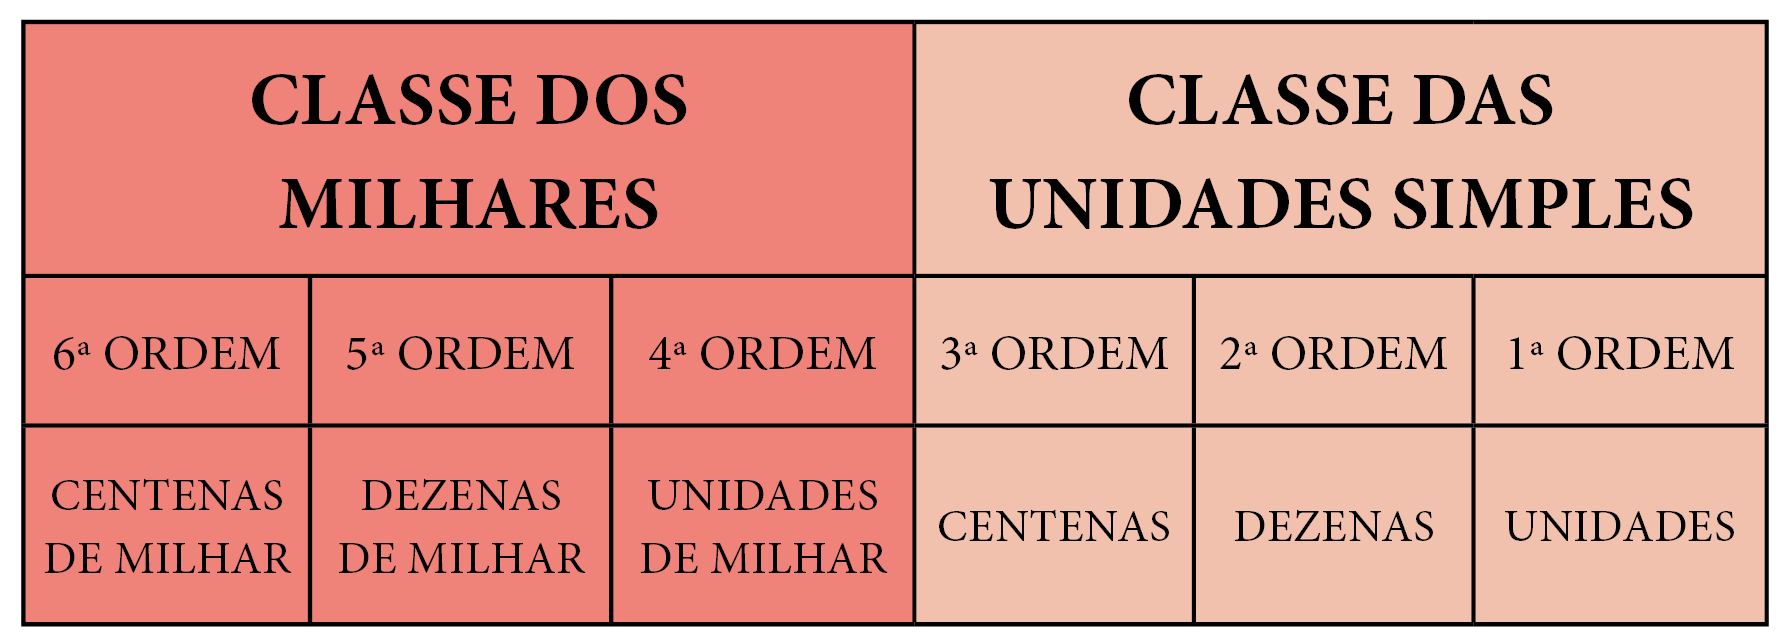
\includegraphics[width=3.55128in,height=1.66618in]{media/image1.png}

Valor posicional ou relativo: é o valor que o algarismo assume
dependendo da classe e da ordem em que ele está posicionado no número.

Exemplo: No número 352.146, o algarismo 5 possui valor posicional ou
relativo igual a 50.000, pois ocupa a 5º ordem, a qual está dentro da
classe dos milhares; ou seja, está na posição da dezena de milhar. Sendo
assim, 5 x 10.000 = 50.000.

Decomposição numérica de acordo com a posição do algarismo:

Exemplo: 389 = 3 x 100 + 8 x 10 + 9}

\colorsec{Atividades}

\num{1} Vilma encontrou um pedaço de papel em sua bolsa com um número escrito:

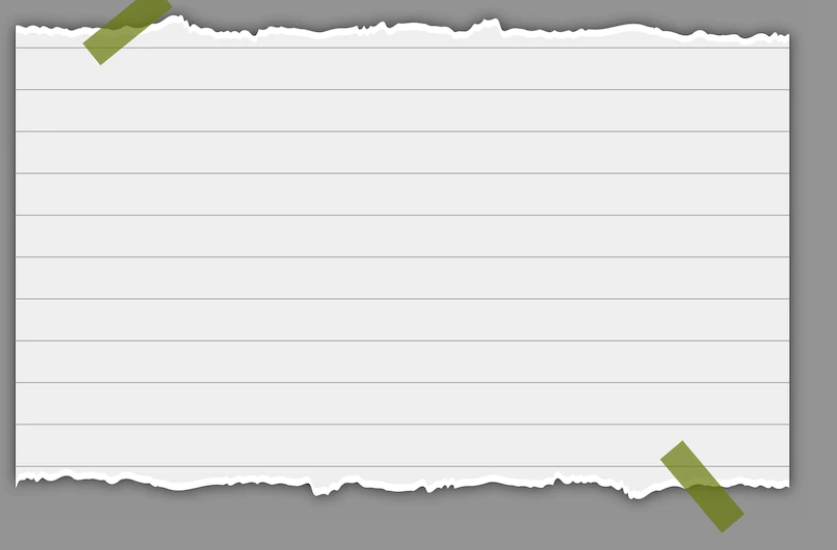
\includegraphics[width=3.30833in,height=2.17391in]{media/image2.png}

\url{https://img.freepik.com/vetores-gratis/vetor-de-fundo-de-design-de-pedaco-de-papel-rasgado_1055-13108.jpg?w=900\&t=st=1677434705~exp=1677435305~hmac=787f679840c02b57af4cb87ef851030bb83880366602641e4486462d6d3553f8}

Escrever o número 46 em um pedaço de papel, produzindo assim, a imagem.

\begin{escolha}

\item
  Escreva por extenso como se lê esse número.
\end{escolha}

%deixar uma linha aqui na frente para resposta

\begin{escolha}

\item
  Se for necessário dividir esse número em grupos de 10, quantos grupos
  conseguiríamos formar?
\end{escolha}

%deixar uma linha aqui na frente para resposta

Resposta:

\begin{escolha}

\item
  Quarenta e seis
\item
  Conseguiríamos dividir em 4 grupos com 10 unidades e sobrariam 6
  unidades. 4 x 10 + 6.
\end{escolha}

\num{2} Arnaldo estava contando suas figurinhas e, para isso, montou 8 grupos com
10 figurinhas mais 4 figurinhas em cada um deles.

\begin{escolha}

\item
  Quantas figurinhas Arnaldo possui?
\end{escolha}

%deixar 3 linhas aqui na frente para resposta

\begin{escolha}

\item
  Como se escreve a quantidade de figurinhas que ele tem por extenso?
\end{escolha}

%deixar uma linha aqui na frente para resposta

Resposta:

\begin{escolha}

\item
  8 x 10 + 4 = 84.
\item
  Oitenta e quatro.
\end{escolha}

\num{3} Treine sua criatividade escrevendo:

\begin{escolha}

  \item Um número formado por três algarismos iguais.
\linhas{1}
\coment{Resposta pessoal. Exemplo: 222.}

  \item Um número formado por três algarismos no qual o 0 (zero) seja o terceiro algarismo.
\linhas{1}
\coment{Resposta pessoal. Exemplo: 390.}

  \item Um número formado por três algarismos diferentes.
\linhas{1}
\coment{Resposta pessoal. Exemplo: 159.}

  \item Um número com mais de três algarismos.
\linhas{1}
\coment{Resposta pessoal. Exemplo: 1.477.}

  \item Mostre os números que você criou para um colega e veja os que ele
  criou também.

\end{escolha}

\num{4}

Escreva os números escritos em cada item e, depois, decomponha esse
número conforme o exemplo.

\item Cento e vinte e sete.

127 = 100 + 20 + 7

\begin{escolha}

\item Trezentos e cinquenta e quatro.

\linhas{1}
\coment{300 + 50 + 4}

\item Duzentos e vinte e oito.

\linhas{1}
\coment{200 + 20 + 8}

\item
  Quatrocentos e setenta e seis.

\linhas{1}
\coment{400 + 70 + 6}

\end{escolha}

\num{5}

Complete a tabela seguindo as instruções.

\begin{longtable}[]{@{}lll@{}}
\toprule
Número escrito por extenso & Número escrito com algarismos & Número
decomposto\tabularnewline
\midrule
\endhead
Quinhentos e vinte e seis & &\tabularnewline
& 435 &\tabularnewline
& & 800 + 30 + 2\tabularnewline
& & 700 + 20 + 9\tabularnewline
\bottomrule
\end{longtable}

Resposta:

Quinhentos e vinte e seis: 526 = 500 + 20 + 6

Quatrocentos e trinta e cinco: 435 = 400 + 30 + 5

Oitocentos e trinta e dois: 832 = 800 + 30 + 2

Setecentos e vinte e nove: 729 = 700 + 20 + 9

\num{6} Gabriel, durante sua aul,a estava aprendendo a montar números utilizando o
material dourado e montou o seguinte número:

%Produzir uma imagem semelhante a essa abaixo com 5 barras de 10 cubinhos cada e 9 cubinhos separados. Deixar a figura melhor apresentável e, se possível, numa cor parecida com o dourado.

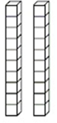
\includegraphics[width=0.47504in,height=1.02509in]{media/image3.png}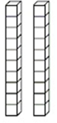
\includegraphics[width=0.47504in,height=1.02509in]{media/image3.png}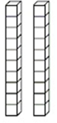
\includegraphics[width=0.47504in,height=1.02509in]{media/image3.png}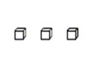
\includegraphics[width=0.75006in,height=0.55838in]{media/image4.png}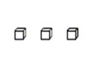
\includegraphics[width=0.75006in,height=0.55838in]{media/image4.png}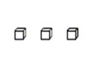
\includegraphics[width=0.75006in,height=0.55838in]{media/image4.png}

Qual é o número representado pelo material dourado na figura?

%deixar 2 linhas aqui na frente para resposta

Resposta:

Temos 6 dezenas e 9 unidades, portanto: 6 x 10 + 9 = 69

\num{7} Complete os quadros abaixo com os número que indicam as quantidades e, em
seguida, escreva por extenso o número encontrado.

\begin{escolha}

\item
  Fernando tem 4 dezenas de lápis mais 2 unidades.
\end{escolha}

\begin{longtable}[]{@{}ll@{}}
\toprule
Dezena & Unidade\tabularnewline
\midrule
\endhead
&\tabularnewline
\bottomrule
\end{longtable}

Total de lápis que Fernando possui: \_\_\_\_\_\_\_\_\_\_\_\_\_\_

\begin{escolha}

\item
  Thiago tem 8 dezenas de bolinhas de gude mais 5 unidades.
\end{escolha}

\begin{longtable}[]{@{}ll@{}}
\toprule
Dezena & Unidade\tabularnewline
\midrule
\endhead
&\tabularnewline
\bottomrule
\end{longtable}

Total de bolinhas de gude que Thiago possui:
\_\_\_\_\_\_\_\_\_\_\_\_\_\_

Resposta:

\begin{escolha}

\item
  4 x 10 + 2 = 42. Quarenta e dois lápis.
\item
  8 x 10 + 5 = 85. Oitenta e cinco bolinhas de gude.
\end{escolha}

\num{8}

Realize a decomposição dos números indicados em cada item.

\begin{escolha}

\item
  56:\_\_\_\_\_\_\_\_\_\_\_\_\_\_\_\_\_\_\_\_\_\_\_\_\_\_\_
\item
  73:\_\_\_\_\_\_\_\_\_\_\_\_\_\_\_\_\_\_\_\_\_\_\_\_\_\_\_\_\_
\item
  94:\_\_\_\_\_\_\_\_\_\_\_\_\_\_\_\_\_\_\_\_\_\_\_\_\_\_\_\_\_\_
\item
  14:\_\_\_\_\_\_\_\_\_\_\_\_\_\_\_\_\_\_\_\_\_\_\_\_\_\_\_\_\_\_
\item
  81:\_\_\_\_\_\_\_\_\_\_\_\_\_\_\_\_\_\_\_\_\_\_\_\_\_\_\_\_\_\_
\item
  158:\_\_\_\_\_\_\_\_\_\_\_\_\_\_\_\_\_\_\_\_\_\_\_\_\_\_\_\_\_\_\_
\item
  649:\_\_\_\_\_\_\_\_\_\_\_\_\_\_\_\_\_\_\_\_\_\_\_\_\_\_\_\_\_\_\_\_
\item
  784:\_\_\_\_\_\_\_\_\_\_\_\_\_\_\_\_\_\_\_\_\_\_\_\_\_\_\_\_\_\_\_\_
\end{escolha}

Resposta:

\begin{escolha}

\item
  5 x 10 + 6 = 56
\item
  7 x 10 + 3 = 73
\item
  9 x 10 + 4 = 94
\item
  1 x 10 + 4 = 14
\item
  8 x 10 + 1 = 81
\item
  1 x 100 + 5 x 10 + 8 = 158
\item
  6 x 100 + 4 x 10 + 9
\item
  7 x 100 + 8 x 10 + 4
\end{escolha}

\num{9} Richard encontrou as seguintes peças de um material dourado:

%Produzir uma imagem semelhante a abaixo mantendo as quantidades pois são importantes para a resolução.

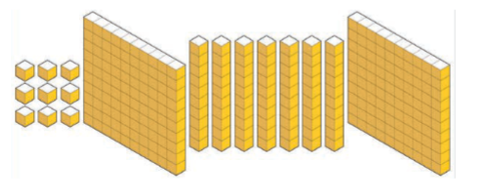
\includegraphics[width=4.02535in,height=1.55013in]{media/image5.png}

Utilizando todas as peças, qual o maior número que Richard conseguirá
representar? Após encontrar o número, escreva-o por extenso.

%Deixar três linhas aqui na frente para resposta

Resposta:

2 x 100 + 7 x 10 + 9 = 279 (Duzentos e setenta e nove)

\num{10}

Monte os números compostos e registre-os nos locais correspondentes.

\begin{escolha}

  \item 5 centenas e 4 unidades:
\linhas{1}
\coment{504}

  \item 7 dezenas e 2 unidades:
\linhas{1}
\coment{72}

  \item 9 centenas, 5 dezenas e 6 unidades:
\linhas{1}
\coment{956}

  \item 2 centenas, 6 dezenas e 3 unidades:
\linhas{1}
\coment{263}

\end{escolha}

\num{11} Ligue os retângulos da coluna 1 a um corresponde da coluna 2 que
represente a escrita por extenso do número indicado na primeira coluna.

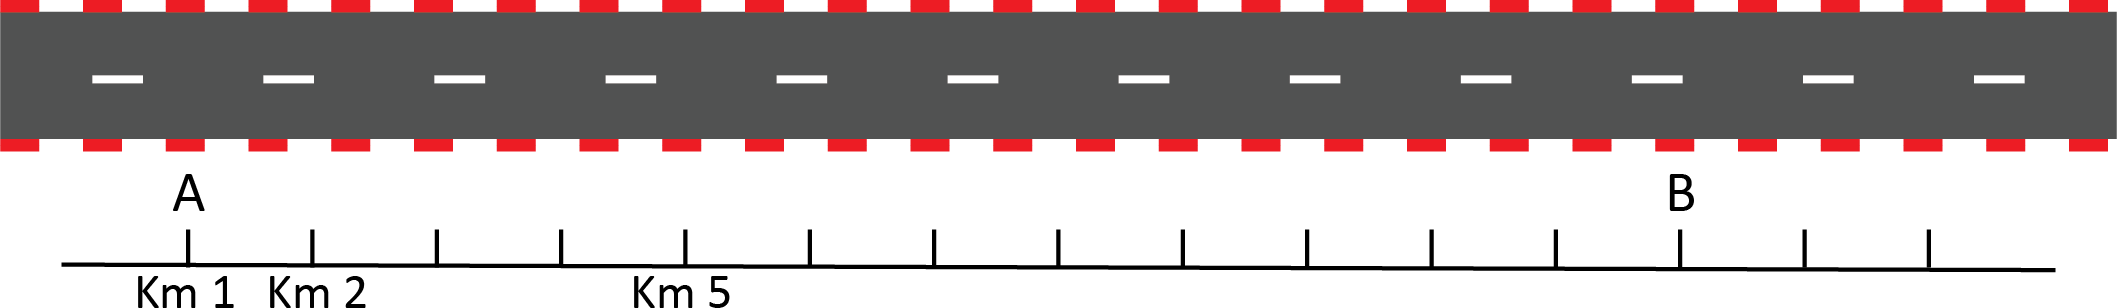
\includegraphics[width=3.85033in,height=1.64181in]{media/image6.png}

%Produzir uma figura conforme a indicada acima: (não colocar os pontos em vermelho que aparecem na figura acima). Não precisa ser colorido. Pose ser feito no padrão e cores do projeto.

Resposta:

88 deve estar ligado ao oitenta e oito.

283 deve estar ligado ao duzentos e oitenta e três.

57 deve estar ligado a ciquenta e sete.

316 deve estar ligado ao trezentos e dezesseis.

\num{12} Felipe quer realizar uma corrida e resolveu planejá-la. Para isso, fez
uma linha reta e nela marcou intervalos de 1 km, conforme representado na imagem.

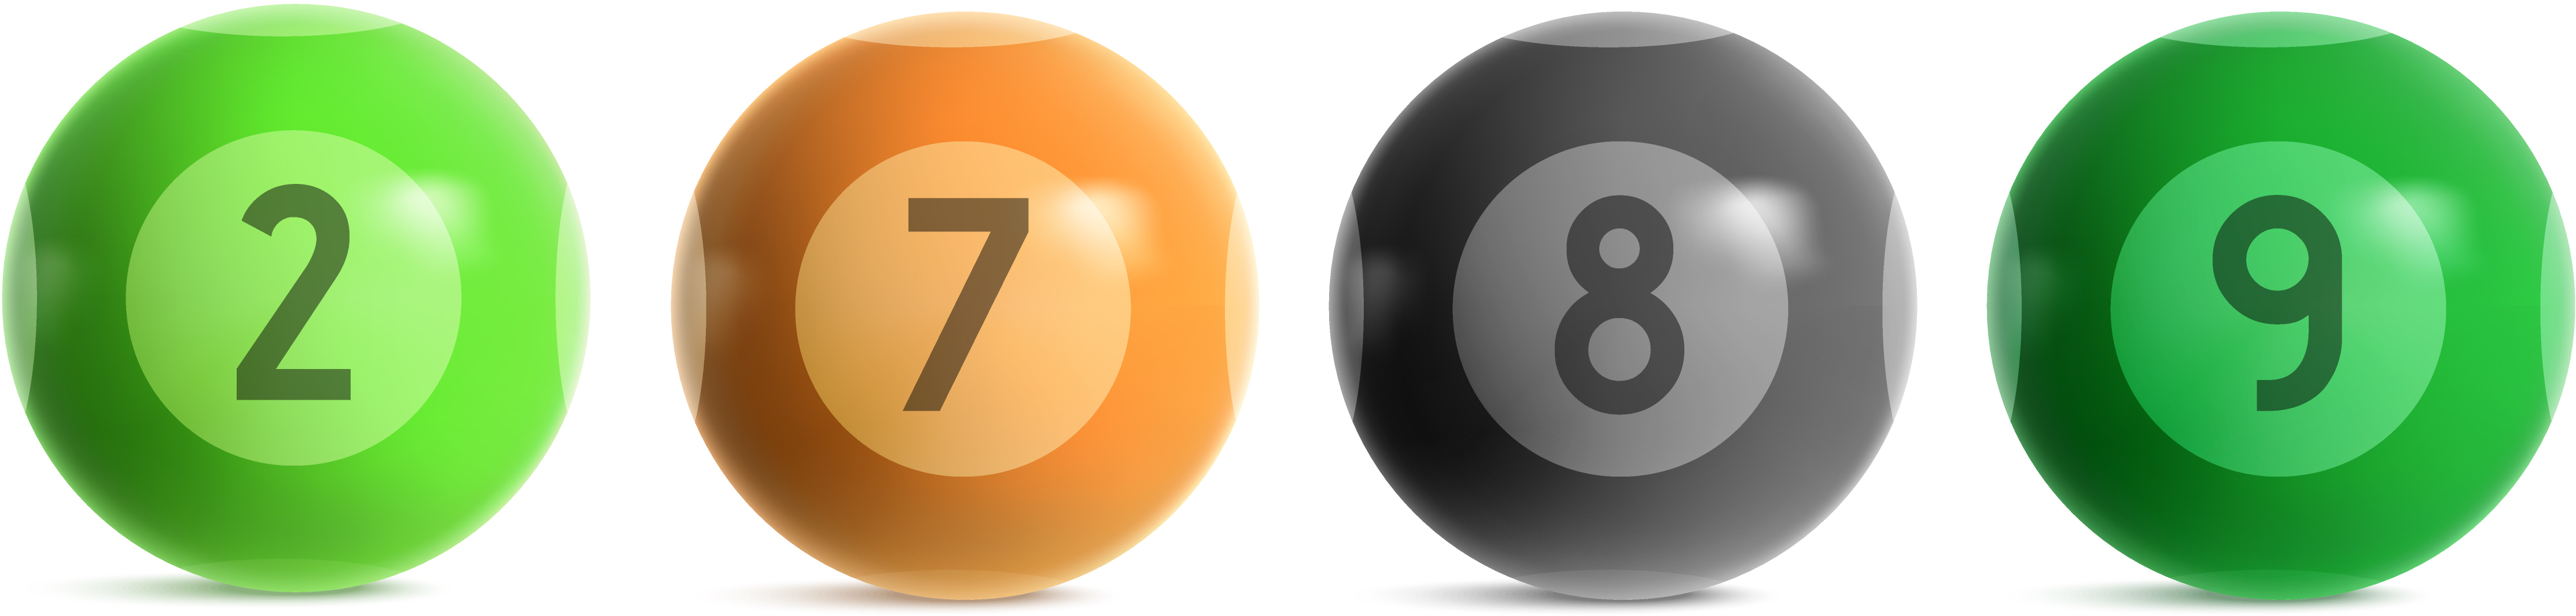
\includegraphics[width=5.90556in,height=0.79514in]{media/image7.png}

%Colocar B no lugar do X no desenho pedido.

%Colocar um desenho de uma pista de corrida com as marcações da forma que estão apresentadas acima. O ponto A deve estar no km 0 e o número de marcações até o ponto B não pode ser alterado.

Ele pretende começar no ponto A e terminar no ponto B. Se Felipe
conseguiu completar a corrida, ele parou na marcação

\begin{escolha}

\item
  Km 9.
\item
  Km 10.
\item
  Km 11.
\item
  Km 12.
\end{escolha}

Resposta:
Como ele saiu do ponto A, que está em cima da marcação km 0, e chegou ao
ponto B, que está a 12 marcações de distância do ponto, podemos concluir
que ele parou no km 12; ou seja, percorreu 12 km.

Explore ao máximo com os alunos a colocação dos números na reta numérica,
já que é um conceito essencial em outros assuntos.

\num{13} A bolas representadas fazem parte de um jogo conhecido como
bilhar ou sinuca.

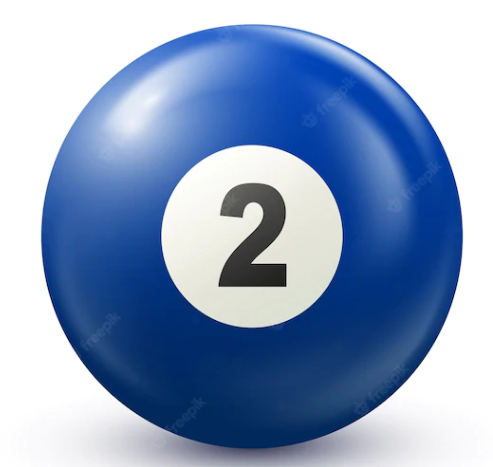
\includegraphics[width=1.40833in,height=1.33406in]{media/image8.png}

\url{https://img.freepik.com/vetores-premium/bola-de-bilhar-azul-com-numero-2-snooker-ou-bola-de-loteria-em-fundo-branco-ilustracao_390775-925.jpg?w=740}

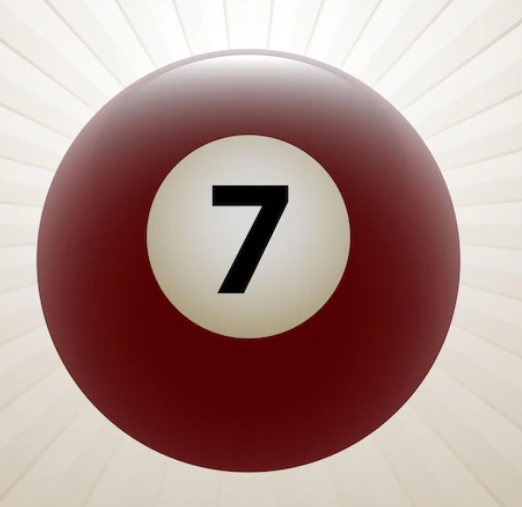
\includegraphics[width=1.66667in,height=1.61877in]{media/image9.png}

\url{https://img.freepik.com/vetores-premium/bilhar_672017-1383.jpg?w=740}

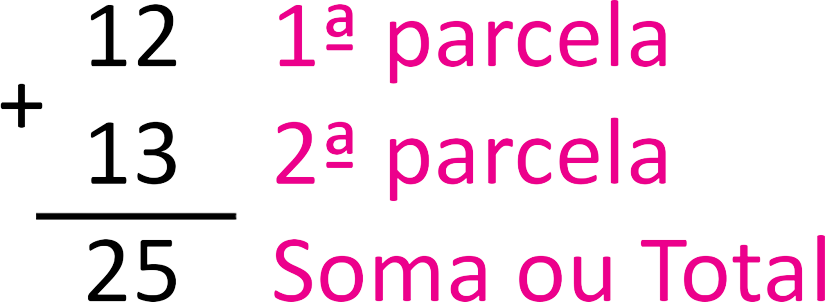
\includegraphics[width=1.68333in,height=1.36449in]{media/image10.png}

\url{https://img.freepik.com/psd-premium/ilustracao-3d-da-bola-de-bilhar-oito_446709-517.jpg?w=740}

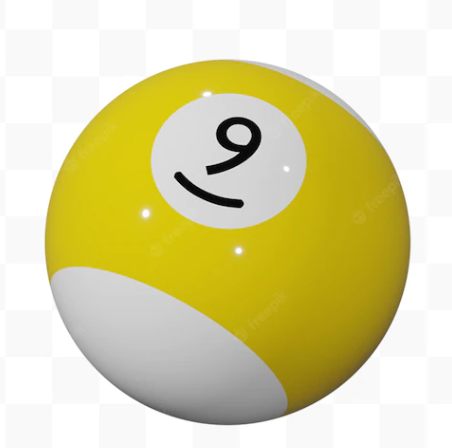
\includegraphics[width=1.61667in,height=1.60236in]{media/image11.png}

\url{https://img.freepik.com/psd-premium/bola-de-bilhar-3d-numero-9_592419-130.jpg?w=740}

%Colocar as bolinhas na mesma linha

Observando os números representados em cada bola, responda:

\begin{escolha}

  \item
  Qual o maior número?
\linhas{1}
\coment{9 (nove)}

  \item
  Qual o menor número com 3 exatamente ordens que podemos formar?
%deixar uma linha aqui na frente para resposta
\linhas{1}
\coment{278 (duzentos e setenta e oito)}

\item
  Qual o maior número par que podemos formar?
\linhas{1}
\coment{9.872 (nove mil oitocentos e setenta e dois)}

\end{escolha}

\coment{Explore mais exemplos com os alunos para estimular a criatividade
e a formação de números.}

\colorsec{Treino}

\num{1} Amanda estava brincando no escritório de seu pai quando
encontrou um pedaço de papel com uma anotação.

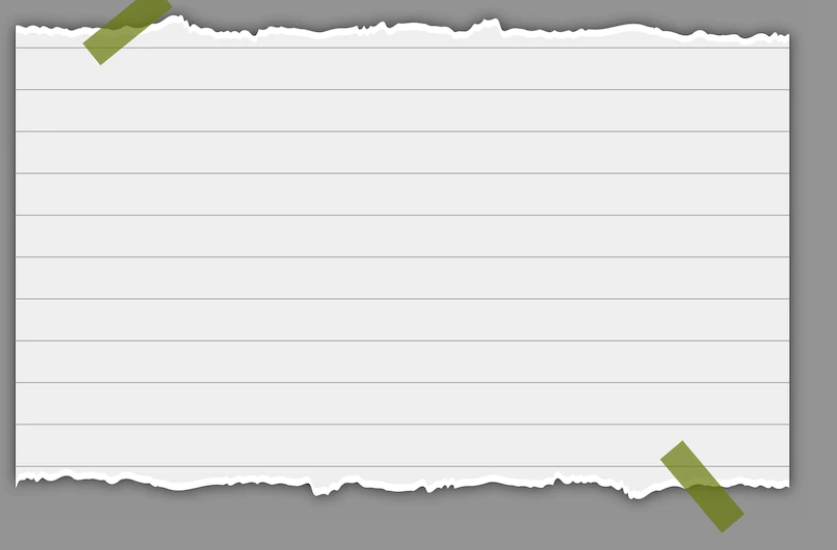
\includegraphics[width=3.30833in,height=2.17391in]{media/image2.png}

\url{https://img.freepik.com/vetores-gratis/vetor-de-fundo-de-design-de-pedaco-de-papel-rasgado_1055-13108.jpg?w=900\&t=st=1677434705~exp=1677435305~hmac=787f679840c02b57af4cb87ef851030bb83880366602641e4486462d6d3553f8}

%Um pedaço de papel com a frase abaixo escrita

Faturamento diário: 734 reais

Lembrando das aulas de matemática, ela resolveu decompor o número escrito
no papel. Qual a decomposição correta que Amanda deverá fazer desse
número?

\begin{escolha}

\item
  700 + 30 + 4
\item
  70 + 3 + 4
\item
  700 + 40 + 3
\item
  70 + 300 + 4
\end{escolha}

Resposta: A

700 + 30 + 4

\num{2} Na reta numérica a seguir, o ponto P representa o número 540 e o ponto U
representa o número 590.

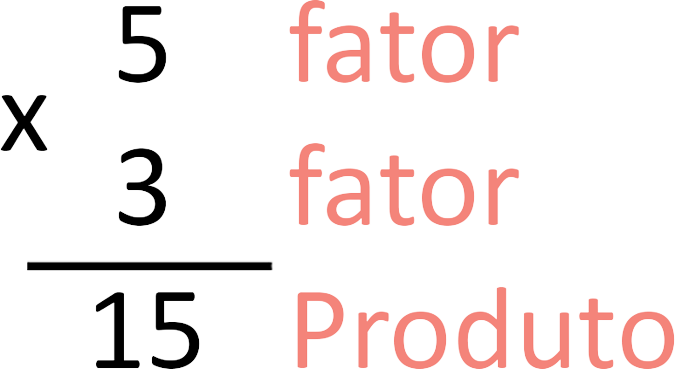
\includegraphics[width=3.03205in,height=0.81228in]{media/image12.png}

%Na figura acima ao invés de 960 favor colocar 540 e no lugar de 1 010 colocar 590.

Em qual ponto temos a representação do número 570, sabendo-se que a
distância entre dois pontos consecutivos é de 10 unidades?

\begin{escolha}

\item
  Q
\item
  R
\item
  S
\item
  T
\end{escolha}

Resposta: C

O 570 estará no ponto S, pois, como no ponto P está o 540 e cada
repartição é de 10 unidades, ele deve estar no terceiro ponto após o P,
sem contar o ponto S.

\num{3} Utilizando o material dourado, Ana Letícia montou a seguinte número:

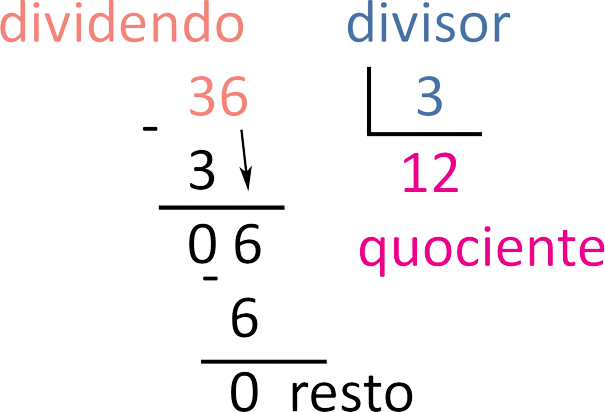
\includegraphics[width=4.13369in,height=0.83341in]{media/image13.png}

%Construir uma figura dessa forma mantendo a quantidade de 5 placas (10 cubinhos x10 cubinhos) e 9 cubinhos pequenos.

Qual o número representado por Ana Letícia?

\begin{escolha}

\item
  59
\item
  159
\item
  509
\item
  1 509
\end{escolha}

Resposta: C

5 x 100 + 1 x 9 = 509.

\chapter{}
\markboth{2. Cálculos}{}

\colorsec{Habilidades do SAEB}

\begin{itemize}
    \item Calcular o resultado de adições ou subtrações envolvendo números
naturais de até 6 ordens.

    \item Calcular o resultado de multiplicações ou divisões envolvendo números
naturais de até 6 ordens.

    \item Associar o quociente de uma divisão com resto zero de um número
natural de até 6 ordens por 2, 3, 4, 5 e 10 às ideias de metade, terça,
quarta, quinta e décima parte.

    \item Resolver problemas de adição ou de subtração, envolvendo números
naturais de até 6 ordens, com os significados de juntar, acrescentar,
separar, retirar, comparar ou completar.

    \item Resolver problemas de multiplicação ou de divisão, envolvendo números
naturais de até 6ordens, com os significados de formação de grupos
iguais (incluindo repartição equitativa e medida), proporcionalidade ou
disposição retangular.
\end{itemize}

\coment{Habilidades da BNCC: EF03MA06, EF03MA07, EF03MA08.}

\conteudo{

\coment{Assim como todos os conteúdos que envolvem as quatro operações básicas, este módulo é essencial e seu estudo deve ser feito com tempo para bastante treino. Relembre com os alunos cada detalhe
e os algoritmos de adição, subtração, multiplicação e divisão, dando 
ênfase à divisão, que geralmente é o maior desafio enfrentado pelos alunos.}

Adição:

%Fazer a imagem abaixo segundo os padrões do projeto.

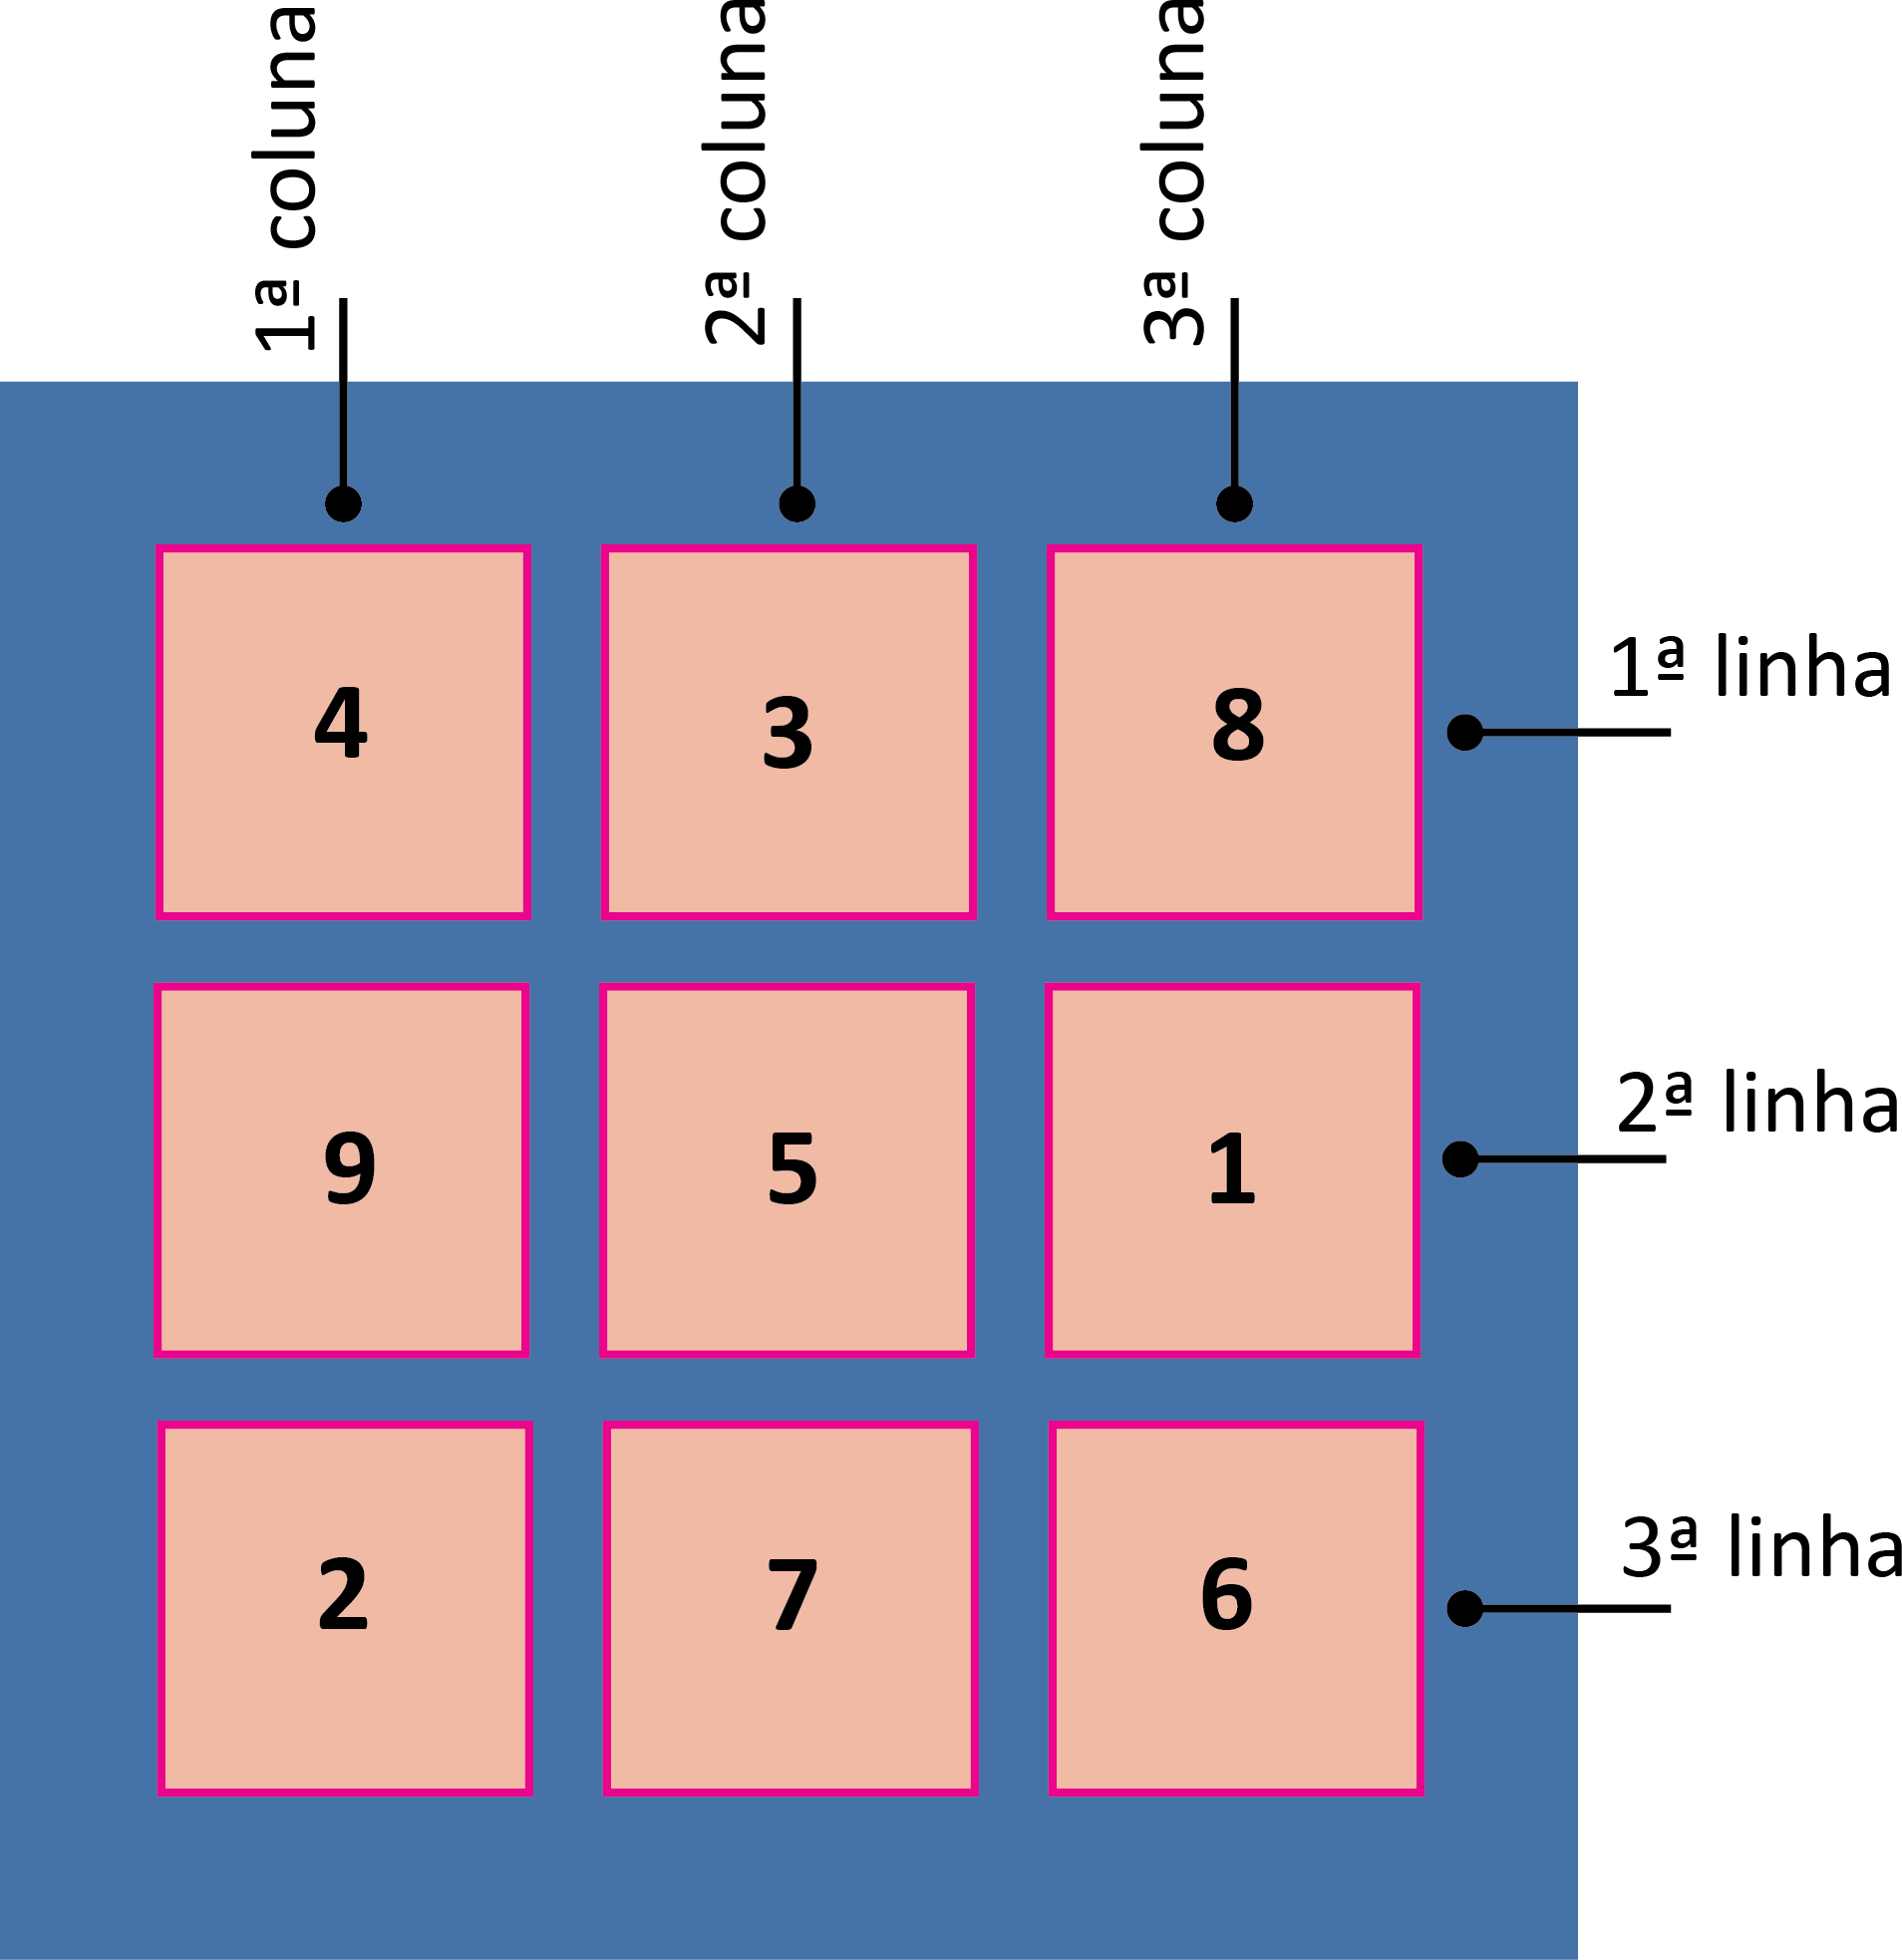
\includegraphics[width=2.26282in,height=1.19473in]{media/image14.png}

Subtração:

%Fazer a imagem abaixo segundo os padrões do projeto.

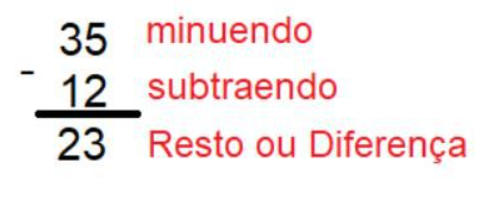
\includegraphics[width=2.55128in,height=1.04961in]{media/image15.png}

Multiplicação:

%Fazer a imagem abaixo segundo os padrões do projeto.

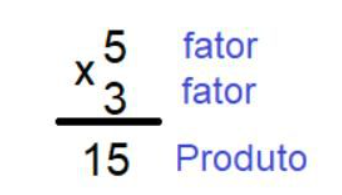
\includegraphics[width=1.92308in,height=1.09649in]{media/image16.png}

Divisão:

%Fazer a imagem abaixo segundo os padrões do projeto.

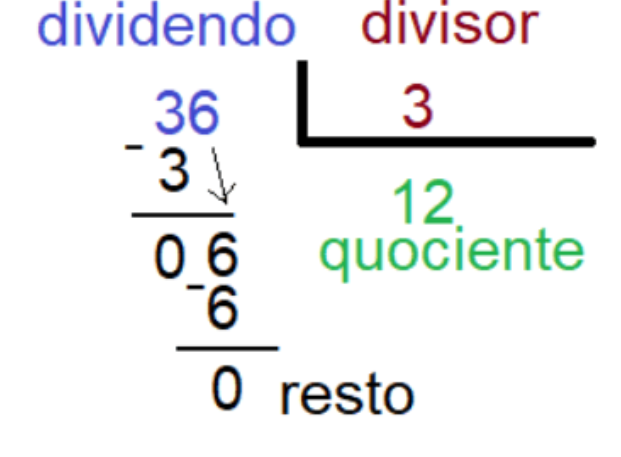
\includegraphics[width=2.26923in,height=1.66995in]{media/image17.png}}

\colorsec{Atividades}

\num{1} Assinale o que deve ser feito em cada item para que ocorra o que se pede.

\begin{escolha}

\item
  Transformar 262 em 362.

\Incluir três alternativas para que o aluno marque uma delas: a) Adicionar 1. b) Adicionar 10. c) Adicionar 100.

\item
  Transformar 1.100 em 1.000.

\Incluir três alternativas para que o aluno marque uma delas: a) Subtrair 1. b) Subtrair 10. c) Subtrair 100.

\item
  Transformar 238 em 239.

\Incluir três alternativas para que o aluno marque uma delas: a) Adicionar 1. b) Subtrair 1. c) Adicionar 10.

\num{2} Utilize os sinais \textless{} (menor que), \textgreater{} (maior que) ou
= (igual a) em cada situação para comparar as quantidade representadas.

\begin{escolha}

\item
  7\_\_\_\_\_\_\_\_\_14
\item
  21\_\_\_\_\_\_\_\_5
\item
  1 + 3\_\_\_\_\_\_\_\_\_2 + 2
\item
  5 + 2\_\_\_\_\_\_\_7 -- 1
\item
  20 -- 1\_\_\_\_\_\_\_\_\_\_19
\item
  Treze\_\_\_\_\_\_\_\_quinze
\end{escolha}

Resposta:

\begin{escolha}

\item
  Menor que, \textless{}
\item
  Maior que, \textgreater{}
\item
  Igual a, =
\item
  Maior que, \textgreater{}
\item
  Igual a, =
\item
  Menor que, \textless{}
\end{escolha}

\num{3} Ligue cada operação que está na coluna 1 com o seu resultado correto na coluna 2.

\Os números 37, 9, 96, 4 e 12 devem aparecer na coluna da direita.

84 + 12                   37

60 -- 23                   9

67 -- 58                    96

50 -- 2 x (5 + 15) + 2      4

2 + 8 -- 2 x (1 + 2)           12

%Colocar as operações acima e os resultados de ambas as colunas em retângulos

%Deixar um espaço em branco  para os alunos efetuarem os cálculos necessários

Resposta:

Explore ao máximo com os alunos o conceito de quais operações
devem ser realizadas primeiro e, assim, ajude na fixação desse conceito.

84 + 12 = 96

60 -- 23 = 37

67 -- 58 = 9

50 -- 2 x (5 + 15) + 2 = 50 -- 40 + 2 = 12

2 + 8 -- 2 x (1 + 2) = 2 + 8 -- 6 = 4

\num{4}

Observe atentamente a figura dada e, em seguida, responda ao que se pede em cada item.

%Produzir uma figura semelhante a abaixo nos moldes do projeto mas os números devem ser os mesmos. 
\Imagino que possa ser feita uma tabela simples.

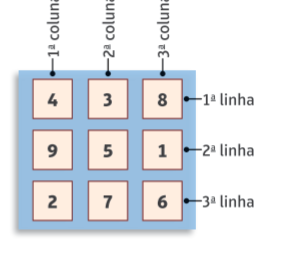
\includegraphics[width=2.37521in,height=2.18352in]{media/image21.png}

\begin{escolha}

\item
  Qual a soma de todos os números que estão na primeira coluna?
\linhass{3}
\coment{4 + 9 + 2 = 15}

\item
  Qual a soma de todos os números que estão na segunda coluna?
\linhass{3}
\coment{3 + 5 + 7 = 15}

\item
  Qual a soma de todos os números que estão na terceira coluna?
\linhass{3}
\coment{8 + 1 + 6 = 15}

\item
  O que você percebe quando compara os resultados da soma dos números de
  cada coluna?
\linhass{3}
\coment{A soma sempre resulta em 15.}

\item
  Qual a soma dos números que estão na 1º linha?
\linhass{3}
\coment{4 + 3 + 8 = 15}

\item
  Qual a soma dos números que estão na 2º linha?
\linhass{3}
\coment{9 + 5 + 1 = 15}

\item
  Qual a soma dos números que estão na 3º linha?
\linhass{3}
\coment{2 + 7 + 6 = 15}

\item
  O que você percebe quando compara os resultados da soma dos números de
  cada linha?
\linhass{3}
\coment{A soma sempre resulta em 15.}
\end{escolha}

\num{5}

Vicente vendeu, em um evento que ocorreu na praça central de uma pequena
cidade do interior do Brasil, 6 sorvetes de chocolate, 8 de morango, 3
de groselha e 5 de creme. Quantas unidades de sorvete Vicente vendeu durante esse evento?

\linhass{3}
\coment{6 + 8 + 3 + 5 = 22 unidades de sorvete foram vendidas por Vicente.}

\num{6}

\Inserir imagem de freepik disponível no link https://br.freepik.com/fotos-premium/nao-ha-nada-que-eu-ame-mais-do-que-assar-foto-recortada-de-uma-mulher-decorando-um-bolo-em-sua-cozinha_27771468.htm#query=making%20cake&position=5&from_view=search&track=robertav1_2_sidr

A receita de um bolo diz que inicialmente devemos colocar 260 g de
farinha de trigo e misturar com outros ingredientes como ovos, açúcar e
leite. Em seguida, devemos colocar mais 135 g de farinha de trigo para a
massa ficar no ponto ideal. Qual foi a quantidade total de farinha
utilizada nessa receita?

%Deixar espaço em branco de 3 linhas para a resolução

Resposta:

260 + 135 = 395 g

\num{7} Raquel sempre amou confeitaria e, por isso, decidiu começar uma pequena empresa que faz doces para festas. Para o próximo final de semana, ela
recebeu a seguinte encomenda por mensagem de texto em seu celular:

Encomenda para a festa da Maria

275 brigadeiros

165 beijinhos

245 cajuzinhos

Calcule o total de unidades de doces que Raquel terá que fazer para entregar essa encomenda.

%Deixar espaço em branco equivalente a 4 linhas para a resolução

Resposta:

275 + 165 + 245 = 685 unidades de doces.

\num{8} Complete o quadro, proposto pela professora Marina, transformando
as adições em multiplicações; em seguida, encontre o resultado. Para isso, siga o modelo.

\begin{longtable}[]{@{}lll@{}}
\toprule
Adição de parcelas iguais & Multiplicação & Resultado\tabularnewline
\midrule
\endhead
8 + 8 + 8 & 3 x 8 & 24\tabularnewline
10 + 10 + 10 + 10 + 10 & &\tabularnewline
6 + 6 + 6 + 6 & &\tabularnewline
5 + 5 + 5 + 5 + 5 + 5 + 5 & &\tabularnewline
12 + 12 + 12 + 12 + 12 & &\tabularnewline
\bottomrule
\end{longtable}

Resposta:

\begin{longtable}[]{@{}lll@{}}
\toprule
Adição de parcelas iguais & Multiplicação & Resultado\tabularnewline
\midrule
\endhead
8 + 8 + 8 & 3 x 8 & 24\tabularnewline
10 + 10 + 10 + 10 + 10 & 5 x 10 & 50\tabularnewline
6 + 6 + 6 + 6 & 4 x 6 & 24\tabularnewline
5 + 5 + 5 + 5 + 5 + 5 + 5 & 5 x 7 & 35\tabularnewline
12 + 12 + 12 + 12 + 12 & 5 x 12 & 60\tabularnewline
\bottomrule
\end{longtable}

\num{9} João
possui uma distribuidora de ovos e acabou de receber 15 caixas com 252
ovos cada uma. Para que João venda essa mercadoria, ele faz embalagens
com 12 ovos cada uma. Quantas embalagens João conseguirá fazer para
colocar à venda utilizando os ovos que acabou de receber em sua distribuidora?

\url{https://img.freepik.com/fotos-gratis/ovos-na-superficie-rosa_58702-1950.jpg?w=1060\&t=st=1677435684~exp=1677436284~hmac=6c6204dcded4c4d80a06169fee49d53df4b2636105a2c7b3dbe5365007ceae9a}

%Deixar espaço em branco equivalente a 3 linhas para os cálculos.

Resposta:

(15 x 252):12 = 315 embalagens com 12 ovos cada uma.

É sempre recomendado escrever a expressão formada pela interpretação do enunciado, pois assim os alunos vão aprendendo a transformar textos em linguagem
matemática.

\num{10} Brenda se deparou com uma divisão em sua prova de matemática. Para esse
cálculo, aparecia o número 5.192 como dividendo e o número 22 como divisor. Sabendo-se que
Brenda acertou essa questão, qual foi o quociente encontrado por ela?

Explore também divisões com dividendos maiores.

%Deixar espaço referente a 4 linhas para o cálculo

Resposta:

5.192 : 22 = 236

\num{11} A mãe de Beatriz comprou uma caixa de bombons para presentear seus
quatro filhos. Na caixa, os bombons estavam distribuídos em 8 fileiras
com 9 bombons em cada. Se ela irá dividir a quantidade total de bombons
igualmente entre seus filhos, quantos bombons Beatriz receberá?

%Deixar espaço referente a 3 linhas para cálculos.

Resposta:

(8 x 9) : 4 = 18 

Beatriz receberá 18 bombons, assim como seus irmãos.

\num{12} Observe a conversa entre Rebeca, Raquel e Renata no sítio do avô de Rebeca.

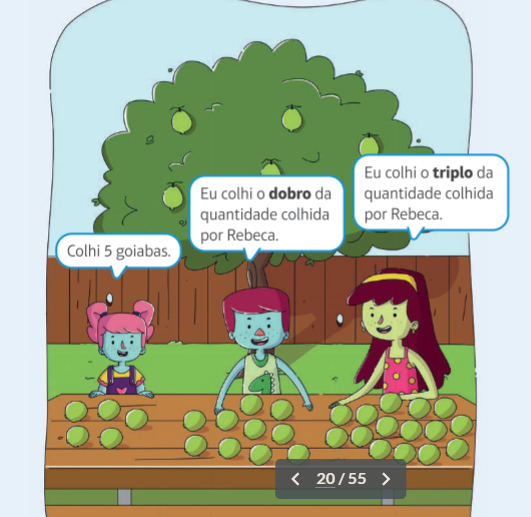
\includegraphics[width=4.42538in,height=4.30871in]{media/image24.png}

%Fazer uma ilustração nos moldes dessa, colocando o nome de cada menina na lateral da mesa a frente delas. Na fala de Renata trocar Rebeca por Raquel. Trocar goiabas por maçãs no texto e nas frutas em cima da mesa. Trocar a palavra dobro na historinha por triplo e aumentar o número de frutas da mesa para 15 na frente dessa menina. Trocar a quantidade frutas na frente da terceira menina para 45.

\begin{escolha}

\item
  Qual a quantidade de maçãs que Rebeca colheu?
\linhass{3}
\coment{5}

\item
  Qual a quantidade de maçãs que Raquel colheu?
\linhass{3}
\coment{3 x 5 = 15}

\item
  Qual a quantidade de maçãs que Renata colheu?
\linhass{3}
\coment{3 x 15 = 45}
\end{escolha}

\num{13}

Complete cada frase com a palavra dobro ou com a palavra triplo.

\begin{escolha}

\item
  O \_\_\_\_\_\_\_\_\_\_ de 10 é 20.
\item
  O \_\_\_\_\_\_\_\_\_\_\_ de 6 é 18.
\item
  O \_\_\_\_\_\_\_\_\_\_\_ de 7 é 14.
\item
  O \_\_\_\_\_\_\_\_\_\_\_\_ de 8 é 24.
\end{escolha}

Resposta:

\begin{escolha}

\item
  dobro
\item
  triplo
\item
  dobro
\item
  triplo
\end{escolha}

\num{14} No quadro branco da professora Adriana foram escritos os seguintes números:

%Construir uma figura conforme a abaixo. Os números importam e devem ser os mesmos.

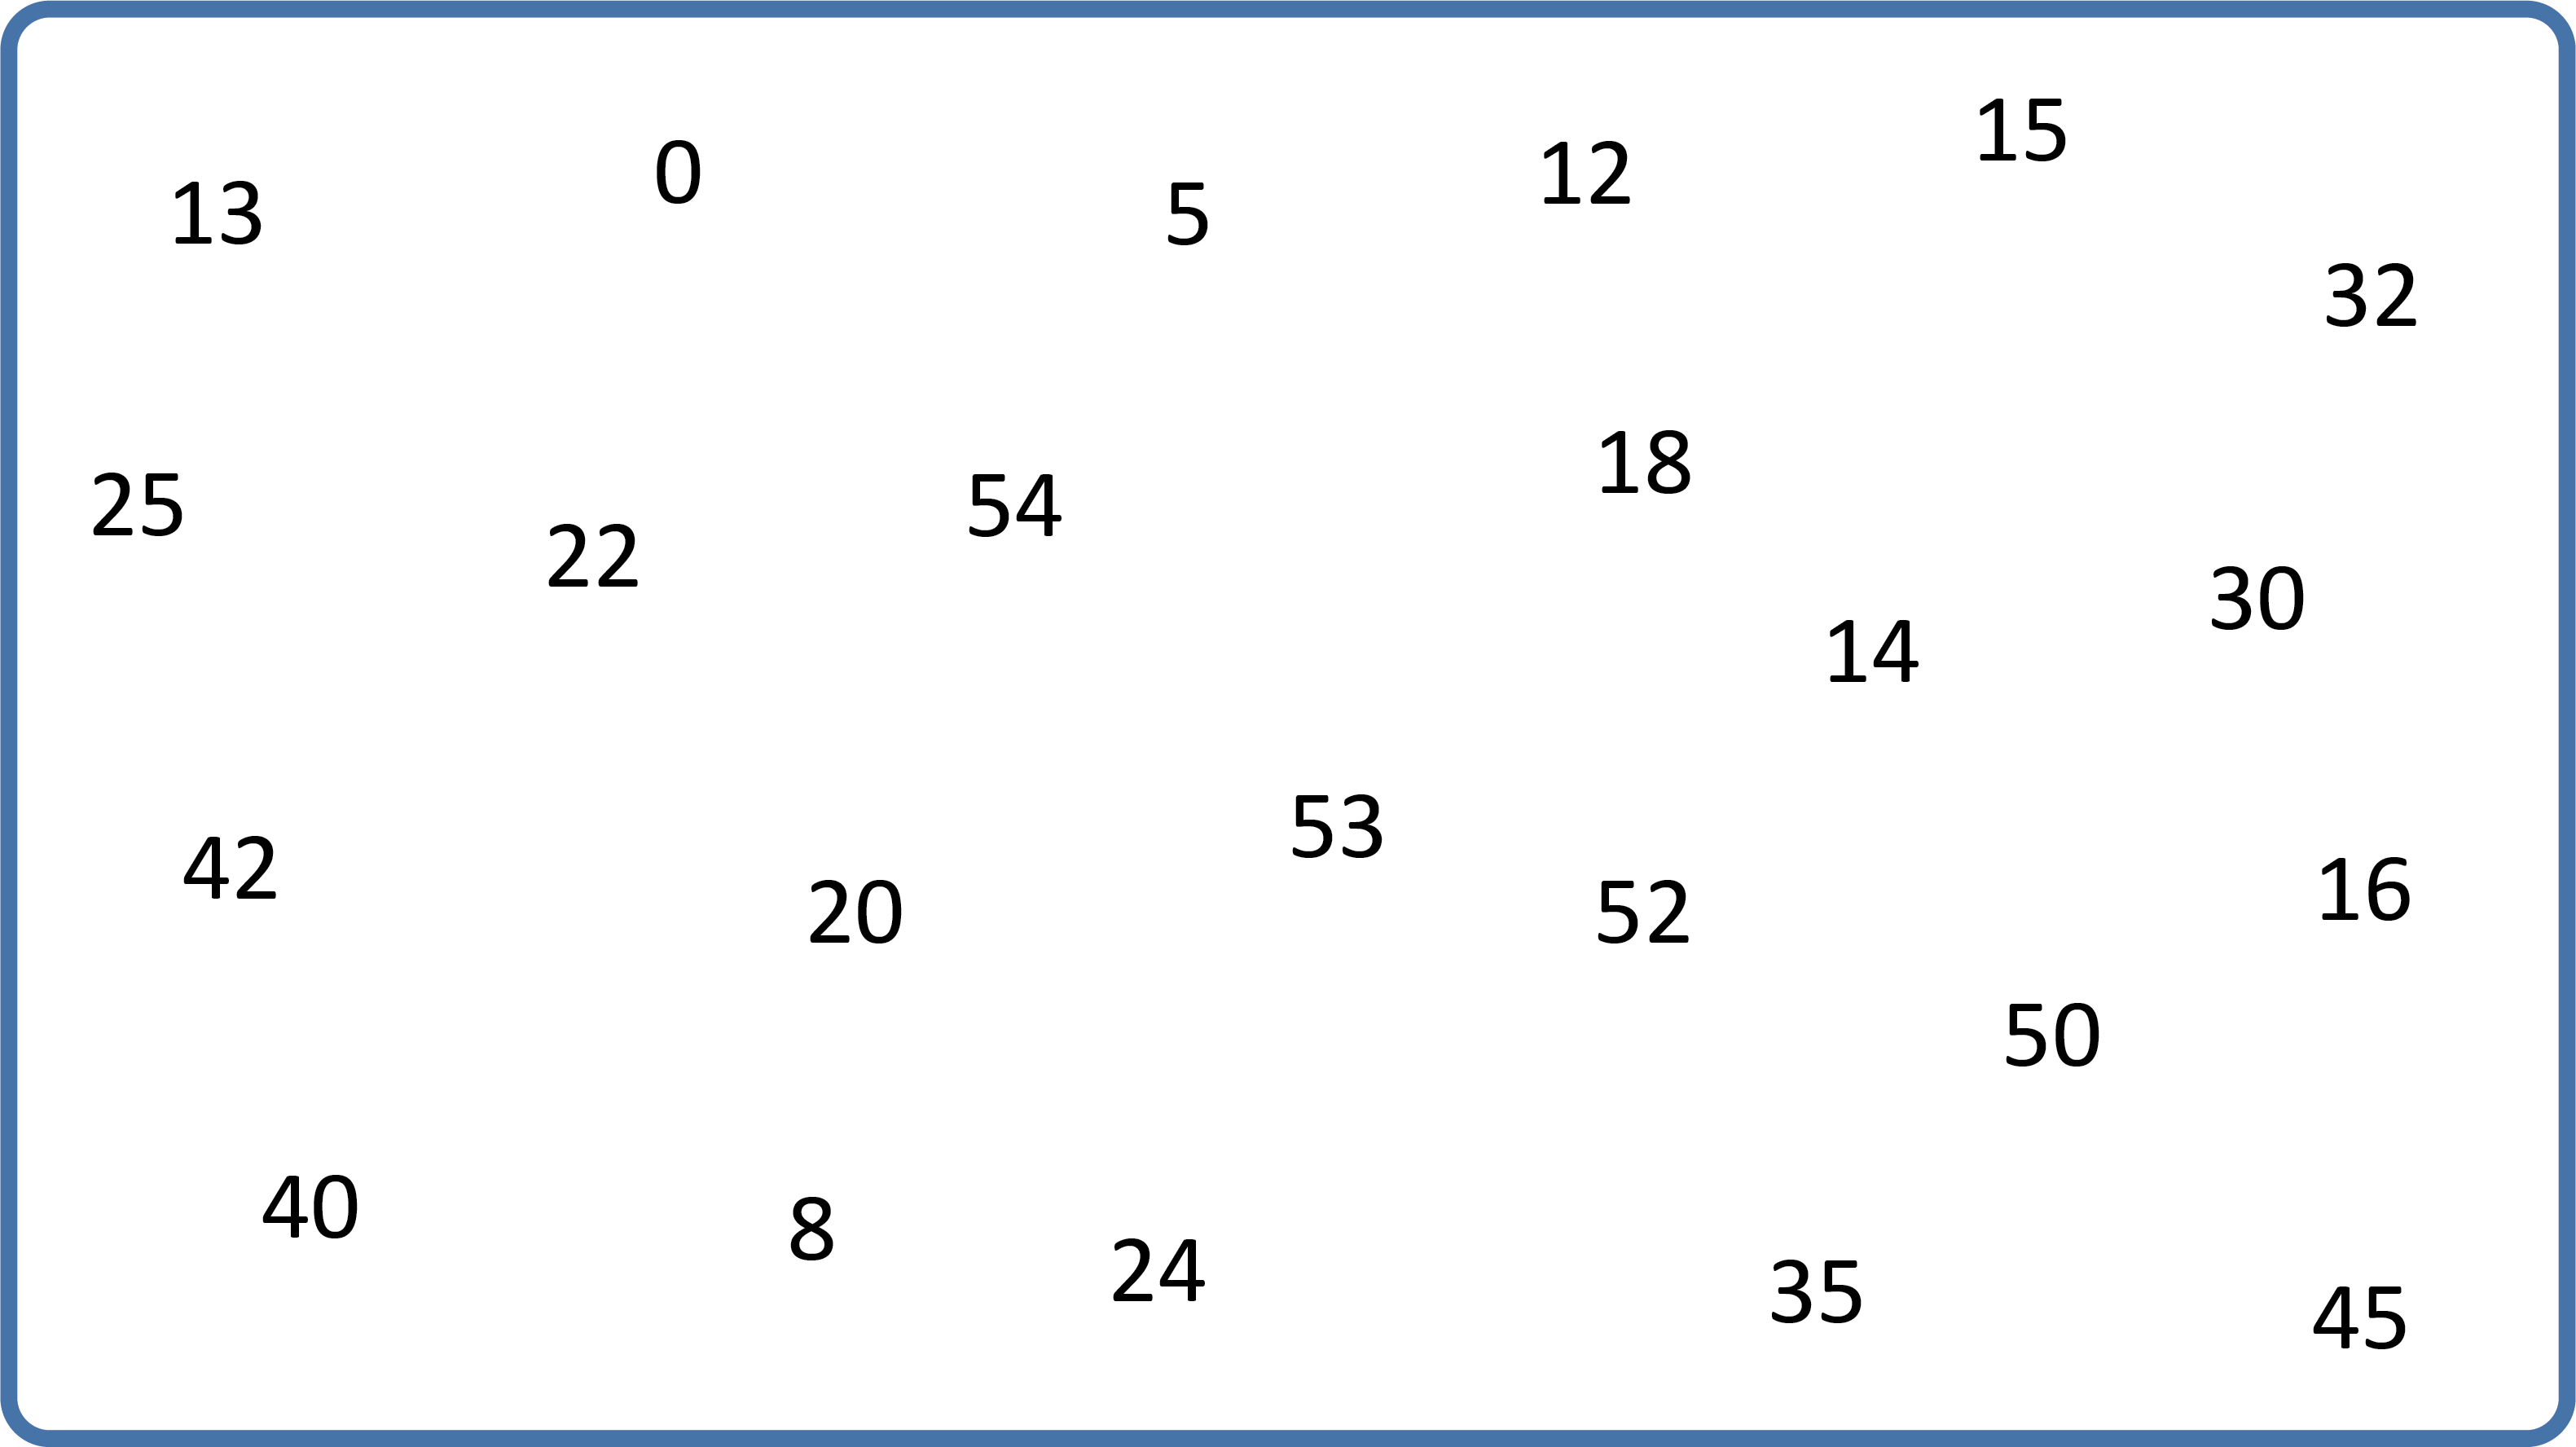
\includegraphics[width=4.51706in,height=2.09185in]{media/image25.png}

Circule aqueles que fazem parte da tabuada do 3.

Resposta:

12; 15; 54; 42; 24; 45.

\colorsec{Treino}

\num{1} Uma costureira pegou uma encomenda para colocar 6 botões em
cada uma das 9 camisas que José utiliza para trabalhar. De quantos botões
ela precisará para concluir a tarefa?

\begin{escolha}
    \item 6
    \item 9
    \item 15
    \item 54
\end{escolha}

Resposta: D

6 x 9 = 54 botões

\num{2} Para uma festa familiar, a mãe de Josué comprou 12 fardos de
suco como os representados pela imagem. Pode-se considerar, então, que, para a festa, foram compradas

\Incluir imagem disponível em https://br.freepik.com/vetores-gratis/latas-em-embalagens-plasticas_11684670.htm#query=six%20pack%20soda&position=0&from_view=search&track=robertav1_2_sidr

\begin{escolha}

\item
  6 latas de suco.
\item
  12 latas de suco.
\item
  72 latas de suco.
\item
  144 latas de suco.
\end{escolha}

Resposta: C

6 x 12 = 72 garrafas.

\num{3} Um campeonato interno de basquete será promovido na escola em que Carlos
estuda. Pelas regras, cada time deverá ter 5 jogadores titulares e mais 3 reservas. Sabendo-se que serão montados 6 times, a quantidade de alunos
que poderão participar do campeonato é igual a

\begin{escolha}

\item
  18
\item
  30
\item
  36
\item
  48
\end{escolha}

Resposta: D

(5 + 3) x 6 = 48 alunos

\chapter{}
\markboth{3. Descobertas e sequências}{}

\colorsec{Habilidades do SAEB}

\begin{itemize}
    \item Inferir ou descrever atributos ou propriedades comuns que os elementos
que constituem uma sequência recursiva de números naturais apresentam.

    \item Inferir o padrão ou a regularidade de uma sequência de números
naturais ordenados, objetos ou figuras.

    \item Inferir os elementos ausentes em uma sequência de números naturais
ordenados, objetos ou figuras.
\end{itemize}

\coment{Habilidade da BNCC: EF03MA10.}

\subsection{Conteúdo}\label{conteuxfado-2}

Uma sequência ou sucessão é um conjunto numérico ordenado, no qual existe sempre uma lógica de formação.

Exemplos:

\begin{itemize}
\item
  A escalação de um time de futebol de salão em ordem alfabética:
\end{itemize}

Alan, Bruno, Fernando, Igor, Tácio.

\begin{itemize}
\item
  Sequência de números naturais pares:
\end{itemize}

(0; 2; 4; 6; 8; 10; 12; ...)

As sequências podem ser classificadas quanto ao número de elementos que apresentam ou podem apresentar.

\begin{itemize}
\item
  Finitas: sequências que apresentam um número de termos bem definido,
  ou seja, 10 termos, 20 termos, 8 termos.
\item
  Infinitas: sequências que apresentam infinitos números de termos, como a sequência dos números naturais.
\end{itemize}

Ainda podemos classificar as sequências em:

\begin{itemize}
\item
  Crescentes: aquelas em que cada termo sucessor é maior que seu antecessor.
\end{itemize}

Exemplo: (5, 10, 15, 20, 25)

\begin{itemize}
\item
  Decrescentes: aquelas em que cada termo sucessor sempre é menor do que seu antecessor.
\end{itemize}

Exemplo: (9, 7, 5, 3)

Antecessor em uma sequência numérica de números naturais: com exceção do zero,
todos os outros termos apresentam um antecessor. O antecessor é o número
imediatamente anterior àquele que está sendo analisado. Exemplo: o
antecessor de 21 é o 20, pois é o número que vem imediatamente antes do 21 na sequência dos números naturais.

Sucessor em uma sequência numérica de números naturais: todos os termos
apresentam um sucessor. O sucessor é o número que aparece imediatamente após o número que está sendo analisado. Exemplo: o sucessor de 21 é o 22, pois é o
número que vem imediatamente depois do 21 na sequência dos números naturais.

\colorsec{Atividades}

\num{1} A professora Mariana colocou seus alunos posicionados em uma fila, iniciada pelo aluno de tênis azul e mochila alaranjada, como na imagem.

\inserir imagem disponível em https://br.freepik.com/fotos-gratis/conjunto-de-estudio-para-criancas-diversas_18411903.htm#query=fila%20de%20crian%C3%A7as&position=12&from_view=search&track=robertav1_2_sidr

Observe atentamente a figura e responda ao que se pede.

\begin{escolha}

  \item Qual a posição na fila da criança que tem uma blusa de bolinhas coloridas?

\linhass{1}
\coment{A criança com blusa de bolinhas coloridas está na 3º posição (terceira posição).}

  \item Qual a posição na fila da criança que tem três estrelas em seu moletom?

\linhass{1}
\coment{A criança com três estrelas no moletom está na 7º posição (sétima posição).}

\end{escolha}

\num{2} O pai de Marcelo mostrou a ele uma sequência de bolinhas pintadas com
diversas cores.

%Produzir uma imagem com essa e as cores importam. Pode ser algo bem simples, Paulo. Veja o original. Assim evitamos sobrecarga nas ilustrações.


\includegraphics[width=2.72524in,height=0.68339in]{media/image28.png}

Observando essa sequência percebemos que a bolinha pintada com a cor
verde escuro é a primeira, enquanto a bolinha pintada com a cor preta é a
última.

Quais as posições das bolinhas pintadas de cor azul?

%deixar 1 linha aqui na frente para resposta

Resposta:

As bolinhas pintadas com a cor azul estão na 5º (quinta) posição e na
14º (décima quarta) posição.

\num{3} Na prova de matemática que Manoela acabou de fazer estava o seguinte exercício:

Escreva uma sequência de números de forma crescente, de 10 em 10, começando no número 705.

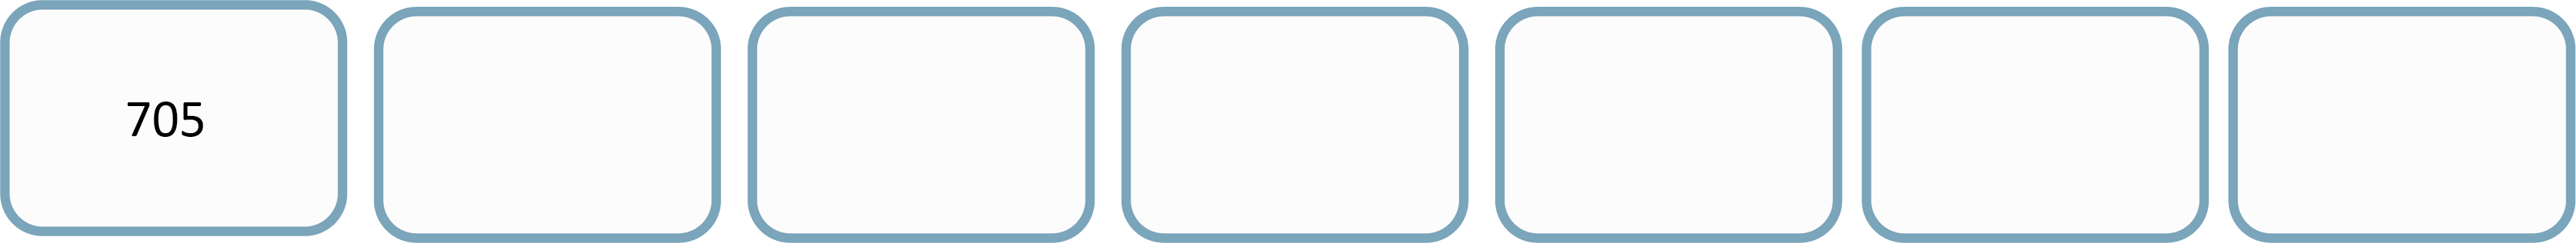
\includegraphics[width=2.95859in,height=1.10010in]{media/image29.png}

%Fazer uma figura conforme a acima, mas no lugar de 809 colocar 705. Além disso colocar os 7 retângulos na mesma linha, ou seja, um ao lado do outro
\também acho que não precisa ir para ilustração, é bem simples de fazer.

Aproveite o exercício que estava na prova de Manoela para estudar.
Escreva dentro de cada retângulo os números que completam a sequência.

%deixar 1 linha aqui na frente para resposta

Resposta:

Sequência:(705; 715; 725; 735; 745; 755; 765)

\num{4} Observe o quadro que Roberta encontrou no caderno de seu irmão.

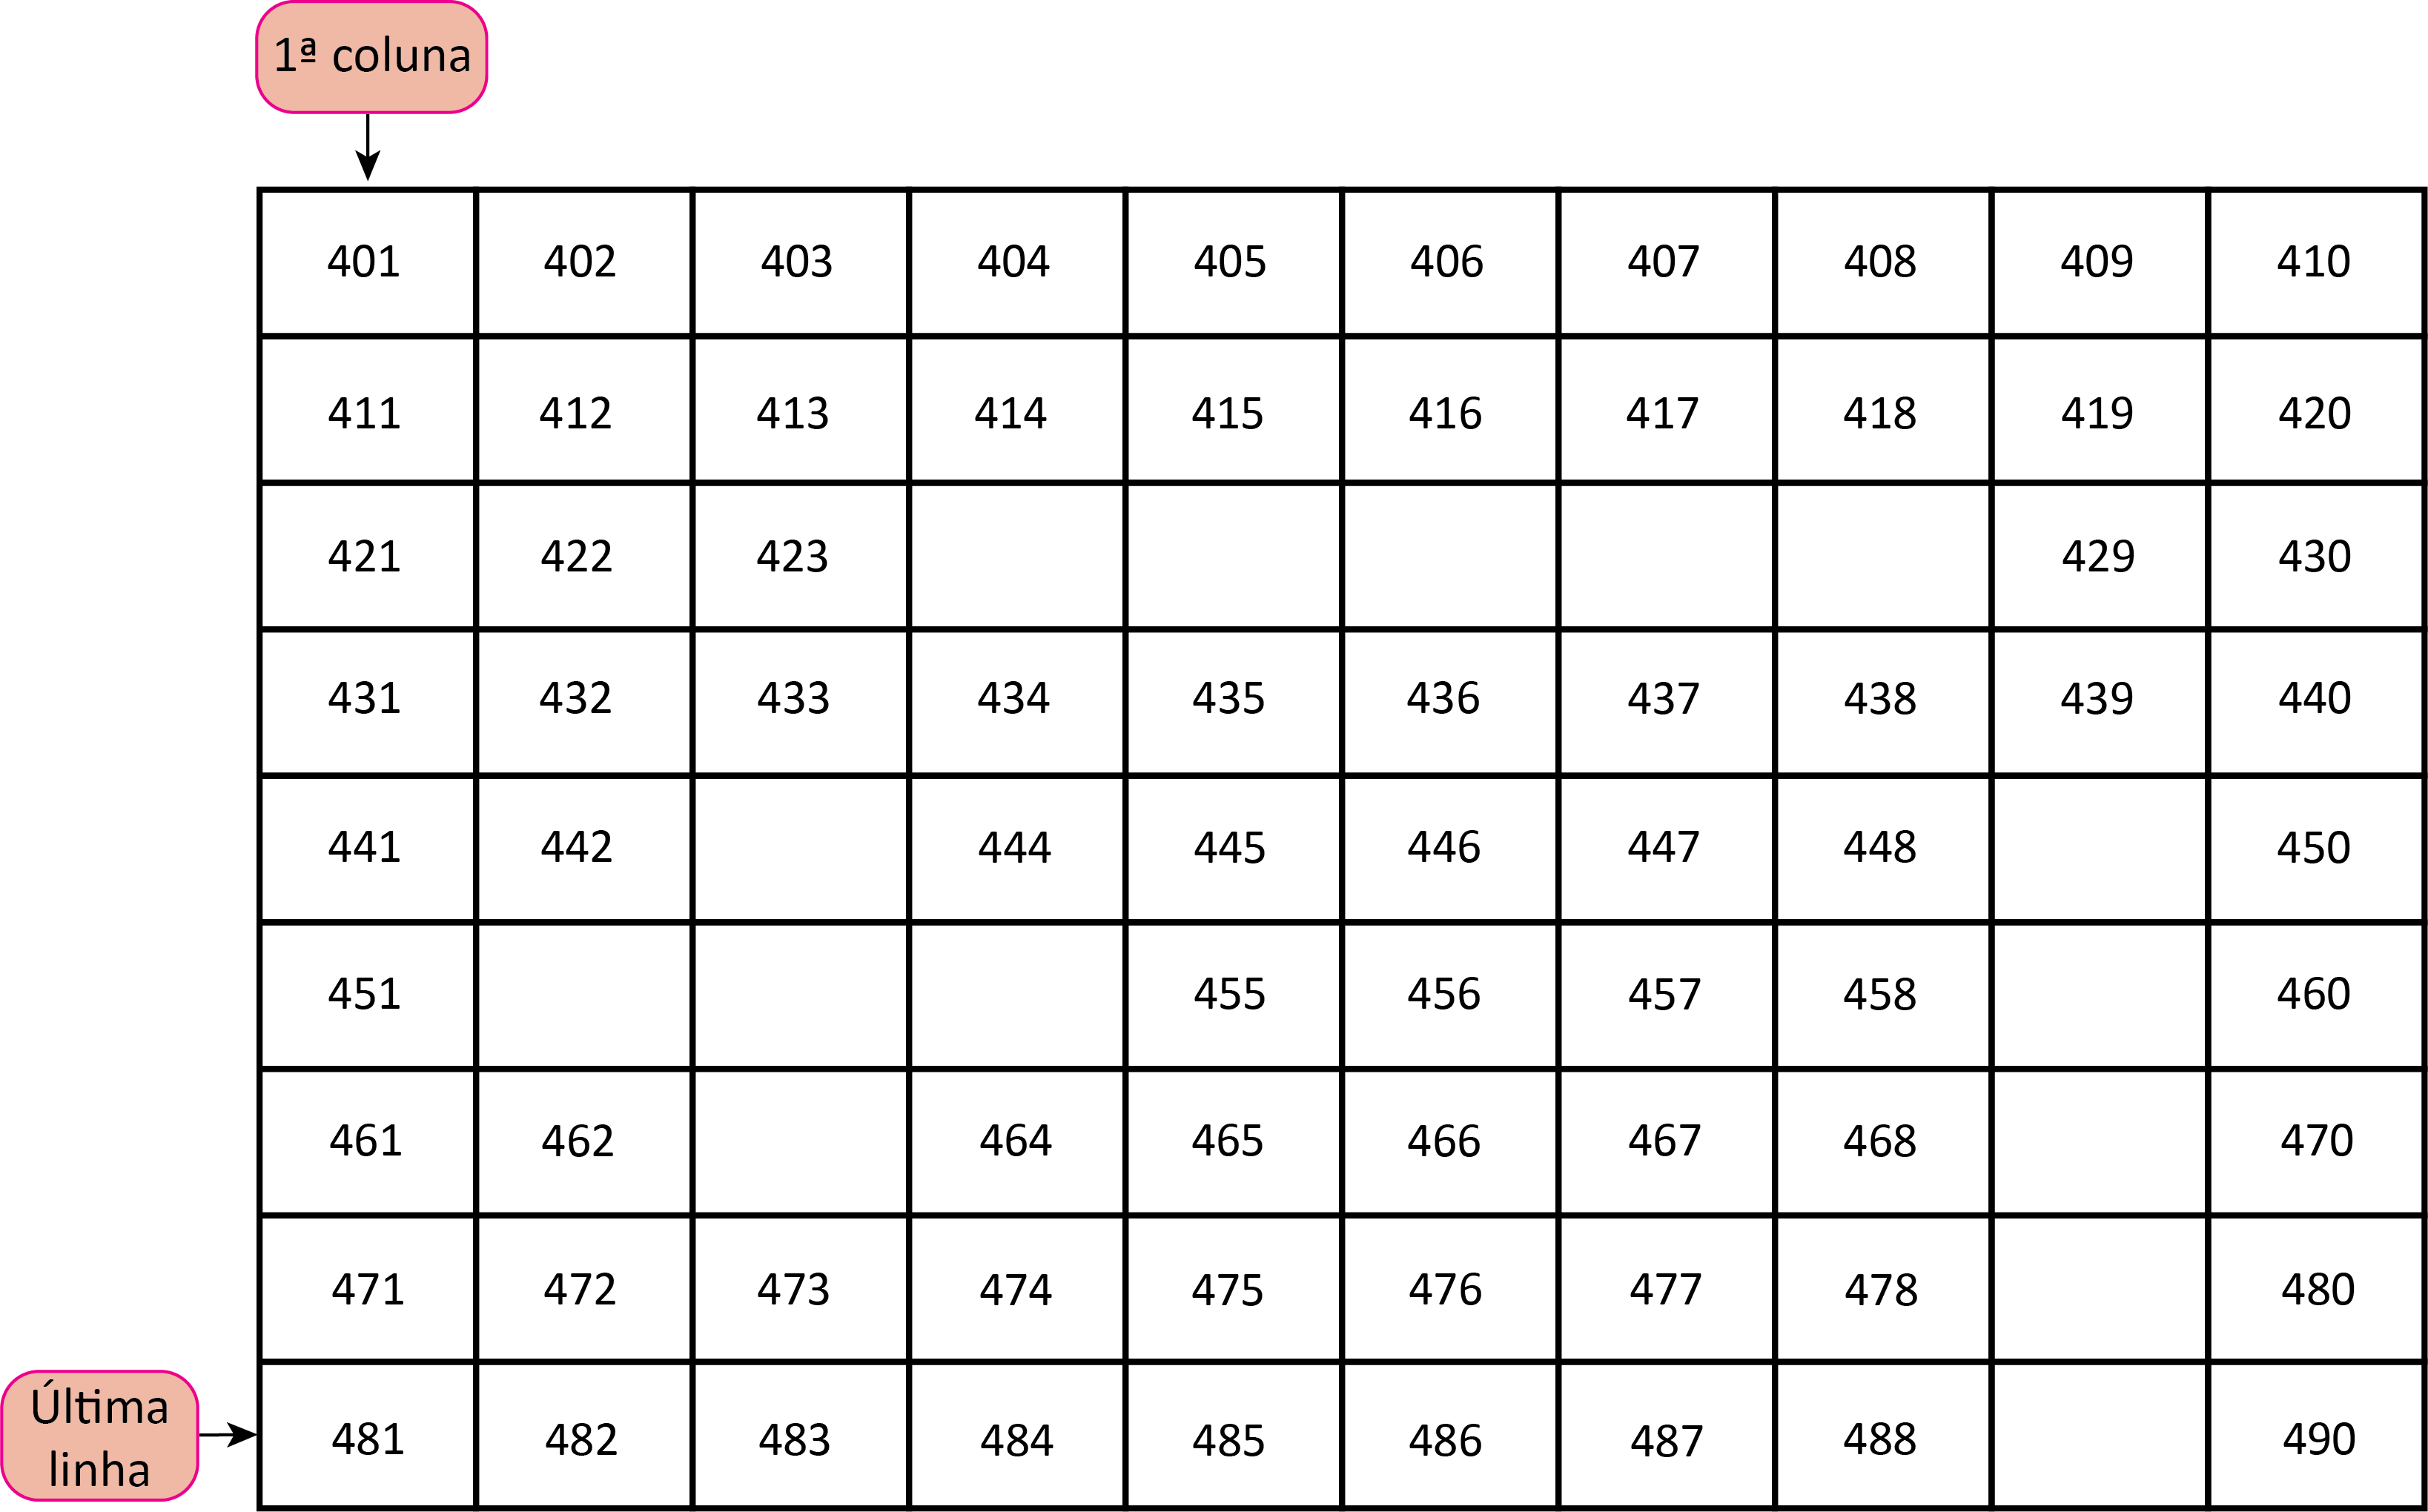
\includegraphics[width=4.05869in,height=3.09193in]{media/image30.png}

%Construir um quadro assim, nos padrões do projeto. Não precisa deixar os espaços coloridos, simplesmente deixar em branco para eles preencherem.
\Consultar o original

\begin{escolha}
\item
  Preencha os espaços vazios como os números que estão faltando.
\coment{
424; 425; 426; 427; 428.

443; 449

452; 453; 454; 459

463; 469

479

489}

\item
  Qual o número que está na 3º coluna e na 4º linha?

\linhas{1}
\coment{433}

\item
  Qual a linha e qual a coluna em que o número quatrocentos e setenta e seis está?

\linhas{1}
\coment{6º coluna e 8º linha.}
\end{escolha}

\num{5}

Alice organizou os nomes dos amiguinhos que pretende convidar para sua
festa de aniversário em uma lista numerada.


1 -- Ana

2 - Ana Clara

3 -- Augusto

4 -- Bernardo

5 -- Camila

6 -- Daniel

Observando atentamente a lista. responda ao que se pede.

\begin{escolha}

\item
  Qual o nome do amigo que aparece na posição do sucessor de 4?
\linhas{1}
\coment{Camila, pois o sucessor de 4 é o 5.}

\item
  Qual o nome do amigo que aparece diante do antecessor de 3?
\linhas{1}
\coment{Ana Clara, pois o antecessor de 3 é o 2.}

\item
  O número diante do qual aparece o nome de Ana é antecessor de qual número?
\linhas{1}
\coment{É Antecessor de 2, já que Ana aparece no número 1.}

\end{escolha}

\num{6} Rafaela foi a uma loja de brinquedos e, para ser atendida, pegou a senha
número 32. Todos são atendidos pela ordem numérica das senhas.

\incluir imagem disponível em https://br.freepik.com/fotos-gratis/mulher-sorridente-segurando-o-cartao-de-visita-em-branco_24488868.htm#query=senha%20de%20atendimento&position=41&from_view=search&track=robertav1_2_sidr

\begin{escolha}

\item
  Qual o número da pessoa que será atendida antes de Rafaela?
\linhass{1}
\coment{O número 31, pois é o antecessor de 32.}

\item
  Qual o número da pessoa que será atendida após Rafaela ser atendida?
\linhass{1}
\coment{O número 33, pois é o sucessor de 32.}

\end{escolha}

\num{7} Observe a reta numérica com números naturais e depois responda a cada item.

%Produzir uma figura como essa, mas melhor apresentável. O número de partes e posição dos números importam.

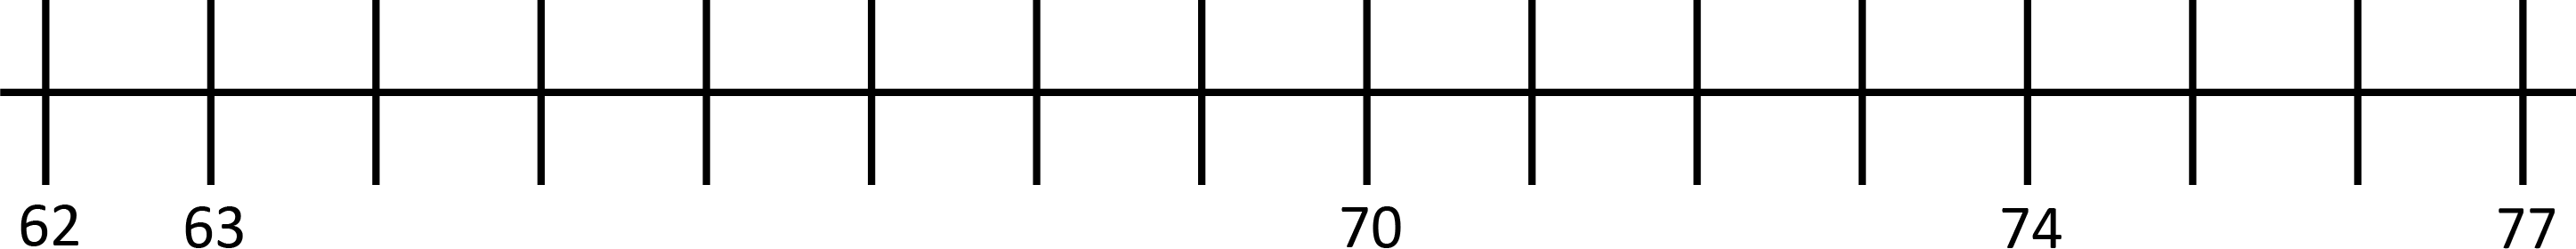
\includegraphics[width=5.22545in,height=0.75840in]{media/image31.png}

\begin{escolha}

\item
  Qual o número natural que será escrito imediatamente após o número 75?
\linhas{1}
\coment{76, pois é o sucessor de 75.}

\item
  Qual o número natural que virá escrito antes do número 68 nessa reta
  numérica?
\linhas{1}
\coment{67, pois é o antecessor de 68.}

\item
  Qual o antecessor do número setenta e sete?
\linhas{1}
\coment{76}

\item
  Qual o sucessor do número setenta e quatro?
\linhas{1}
\coment{75}

\end{escolha}

\num{8} Escreva os números naturais escritos em cada item em ordem crescente.

\begin{escolha}

\item
  30; 25; 10; 5; 20; 15
\linhas{1}
\coment{5; 10; 15; 20; 25; 30}

\item
  7; 21; 14; 35; 28
\linhas{1}
\coment{7; 14; 21; 28; 35}

\item
  16; 8; 12; 4; 24; 20
\linhas{1}
\coment{4; 8; 12; 16; 20; 24}

\end{escolha}

\num{9} Em cada item, indique se a sequência é crescente ou decrescente.

\begin{escolha}

\item
  10; 8; 6; 4; 2; 0
\linhas{1}
\coment{Decrescente.}

\item
  10; 20; 30; 40; 50
\linhas{1}
\coment{Crescente.}

\item
  21; 19; 17; 15; 13
\linhas{1}
\coment{Decrescente.}

\item
  6; 12; 18; 24; 30; 36
\linhas{1}
\coment{Crescente.}

\end{escolha}

\num{10} Observe as sequências dadas e determine, sem fazer desenhos, a
quantidade de bolinhas que a figura 8 de cada sequência terá.

\Paulo, acho que é possível evitar passar esta demanda pala a ilustração, já que é simples. Confira o original e avalie se é viável.

\begin{escolha}

\item
  \_\_\_\_25\_\_\_\_\_\_\_\_bolinhas
\end{escolha}

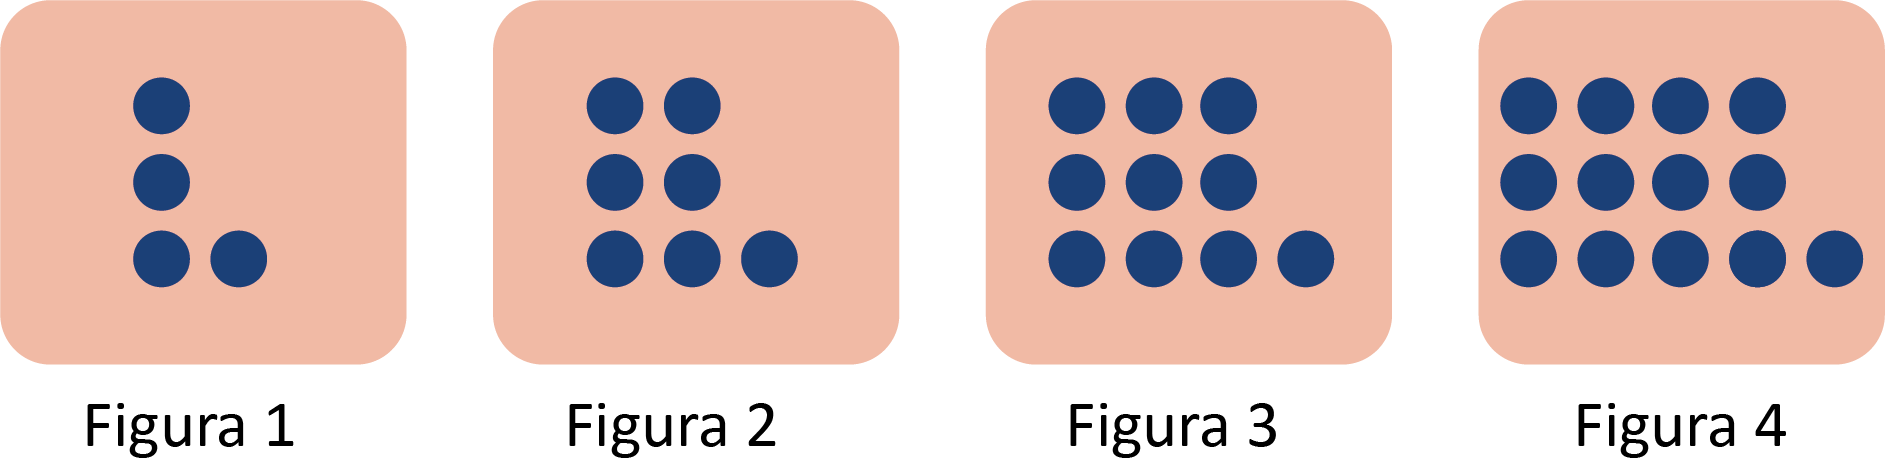
\includegraphics[width=4.09202in,height=0.85841in]{media/image32.png}

%Deixar um espaço em branco equivalente a 2 linhas para resolução.

Resposta:

(4; 7; 10; 13; 16; 19; 22; 25)

\begin{escolha}

\item
  \_\_\_\_24\_\_\_\_\_\_\_\_bolinhas
\end{escolha}

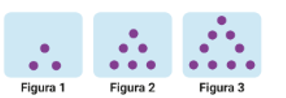
\includegraphics[width=2.38354in,height=0.81674in]{media/image33.png}

%Deixar um espaço em branco equivalente a 2 linhas para resolução.

Resposta:

(3; 6; 9; 12; 15; 18; 21; 24)

\begin{escolha}

\item
  \_\_\_\_\_\_32\_\_\_\_\_\_bolinhas
\end{escolha}

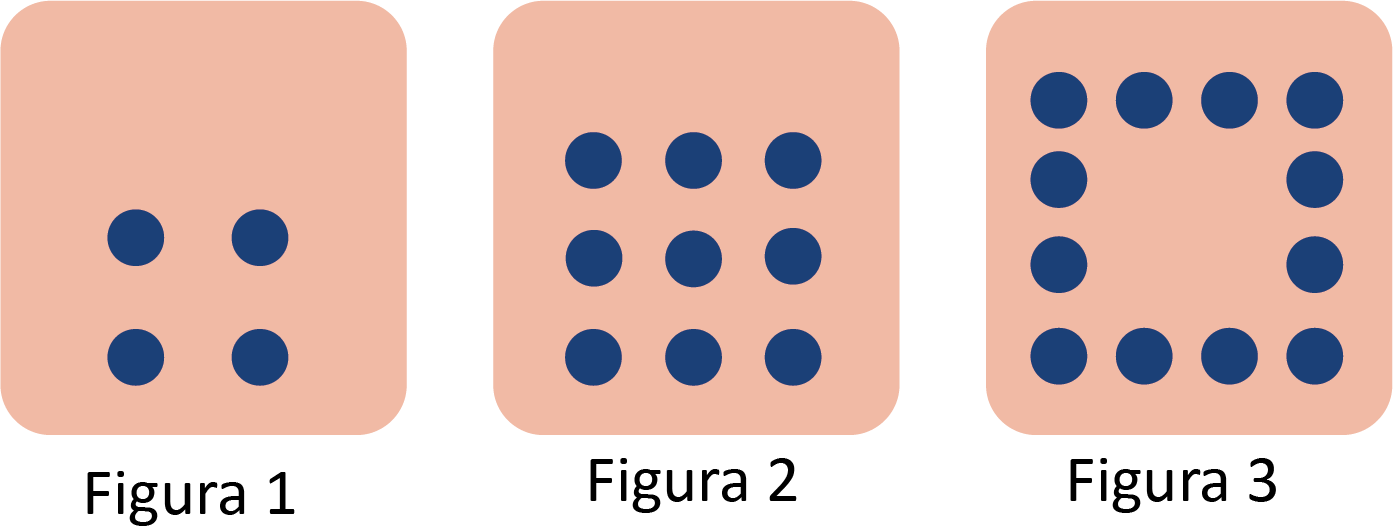
\includegraphics[width=2.38354in,height=0.85007in]{media/image34.png}

%Deixar um espaço em branco equivalente a 2 linhas para resolução.

Resposta:

(4; 8; 12; 16; 20; 24; 28; 32)

\begin{escolha}

\item
  \_\_\_\_\_40\_\_\_\_\_\_\_bolinhas
\end{escolha}


\includegraphics[width=2.35854in,height=0.94175in]{media/image35.png}

%Deixar um espaço em branco equivalente a 2 linhas para resolução.

Resposta:

(5; 10; 15; 20; 25; 30; 35; 40)

\num{11} Encontre o número pedido em cada item.

\begin{escolha}

\item
  O sucessor de 4.089.\_\_\_\_4.090\_\_\_\_\_\_\_\_\_
\item
  O antecessor de 4.302 \_\_\_4.301\_\_\_\_\_\_\_\_
\item
  O sucessor e o antecessor do número 5.259.\_\_5.258 e 5.260.\_\_\_\_\_\_\_\_
\end{escolha}

Resposta:

\begin{escolha}

\item
  4.090
\item
  4.301
\item
  Antecessor: 5.258; sucessor: 5.260.
\end{escolha}

Vale explorar bastante os conceitos de sucessor e antecessor com
os alunos, pois isso facilitará muitos entendimentos em anos futuros.

\num{12} Ana Clara encontrou um papel abaixo entre os cadernos de seu irmão mais velho, com as seguintes anotações:

(21; 58; 95; 132; ...)

Ela ficou muito curiosa, pois entendeu que essa era uma sequência
numérica e queria encontrar o próximo número dessa sequência.

Ajude Ana Clara a descobrir qual é o próximo número da sequência e escreva-o no espaço disponível.

\linhas{1}

Resposta:

A sequência foi montada sempre somando 37 ao número anterior para
encontrar o próximo. Portanto, o próximo número da sequência será: 132 + 37 = 169.

\num{13} A professora de Camila decidiu propor um desafio à turma. Assim, apresentou uma sequência de figuras e pediu que os alunos descobrissem qual seria a próxima imagem. 

\Usar recortes da imagem disponível em https://br.freepik.com/vetores-gratis/cartoes-de-jogo-de-memoria-desenhados-a-mao_37451777.htm#query=sequ%C3%AAncias%20de%20figuras&position=0&from_view=search&track=robertav1_2_sidr  
para construir a seguinte sequência:

bola-quadrado-quadrado-losango-triângulo-triângulo-triângulo-oval-bola-quadrado-quadrado-losango-triângulo

Quem acertou o desafio foi o colega de Camila, Gabriel. Qual foi a resposta dele?

\linhas{3}

Resposta:
Gabriel respondeu que a próxima figura seria um triângulo.

É possível que o aluno continue a sequência com desenhos até chegar à resposta. Não há problemas na utilização dessa técnica.


\num{14} Observe as sequências e complete-as com os números que estão faltando.

\begin{escolha}

\item
\end{escolha}

\begin{longtable}[]{@{}llllll@{}}
\toprule
102 & & 106 & & 110 &\tabularnewline
\bottomrule
\end{longtable}

\begin{escolha}

\item
\end{escolha}

\begin{longtable}[]{@{}llllll@{}}
\toprule
85 & & & 100 & 105 &\tabularnewline
\bottomrule
\end{longtable}

Resposta:

\begin{escolha}

\item
  (102; 104; 106; 108; 110; 112)
\item
  (85; 90; 95; 100; 105; 110)
\end{escolha}

\colorsec{Treino}

\num{1} Se os números escritos a seguir foram colocados em ordem crescente, qual
será o número que ficará imediatamente antes de 63?

Colocar cada um desses números dentro de um círculo e na mesma linha.

95; 63; 25; 76; 54; 68; 48.

\begin{escolha}

\item
  25
\item
  48
\item
  54
\item
  68
\end{escolha}

Resposta: C

Colocando os números em ordem crescente, teremos:

25; 48; 54; 63; 68; 76; 95. Sendo assim, o número que aparece imediatamente antes do 63 é o 54.

\num{2} Observe a sequência e marque a alternativa que corresponde ao número de bolinhas que a figura 6 terá.

%Construir uma figura conforme a abaixo nos padrões do projeto
\Paulo, observando o original, acho que é possível fazer de forma bem simples as representações, sem precisar passar para a ilustração.

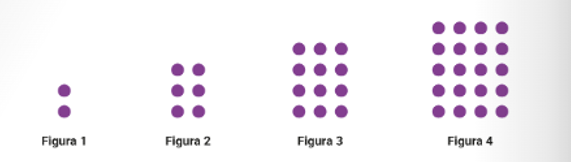
\includegraphics[width=4.75875in,height=1.35012in]{media/image37.png}

\begin{escolha}

\item
  25
\item
  30
\item
  35
\item
  42
\end{escolha}

Resposta: D

(2; 6; 12; 20; 30; 42)

Em cada imagem, aumenta uma bolinha em cada coluna e aumenta em 1 o número de colunas. Assim, teremos: 2; 3 x 2; 4 x 3; 5 x 4; 6 x 5; 7 x 6.

\num{3} Assinale a alternativa que possui uma sequência que traz um antecessor, um número e seu sucessor.

%Criar alternativas
a) 450 - 455 - 460
b) 526 - 626 - 726
c) 436 - 437 - 438
d) 488 - 489 - 490

Resposta: D
Antecessor de um número: Número imediatamente anterior a um número na sequência dos números naturais.
Sucessor de um número: Número imediatamente a frente, ou após, de um número na sequência dos números naturais.

\chapter{}
\markboth{Módulo 4}{}

\coment{Habilidades da BNCC: EF03MA19, EF03MA20}

\colorsec{Habilidades do SAEB}

\begin{itemize}
    \item Reconhecer a unidade de medida ou o instrumento mais apropriado para
medições de comprimento, área, massa, tempo, capacidade ou temperatura.

    \item Estimar/inferir medida de comprimento, capacidade ou massa de objetos,
utilizando unidades de medida convencionais ou não ou medir comprimento,
capacidade ou massa de objetos.

    \item Explicar que o resultado de uma medida depende da unidade de medida
utilizada.

    \item Resolver problemas que envolvam medidas de grandezas (comprimento,
massa, tempo e capacidade) em que haja conversões entre as unidades mais
usuais.

    \item Determinar o horário de início, o horário de término ou a duração de
um acontecimento.
\end{itemize}

Professor durante todo esse módulo trabalhe com os alunos outras
unidades e medidas não tratadas nos exercícios como, por exemplo,
jardas, alqueire, hectare milhas, milhas náuticas, medidas de som entre
outras.

\conteudo{

Construir os quadros abaixo seguindo o padrão de cores do material.

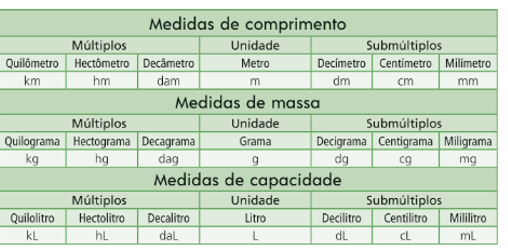
\includegraphics[width=4.23370in,height=2.06685in]{media/image39.png}

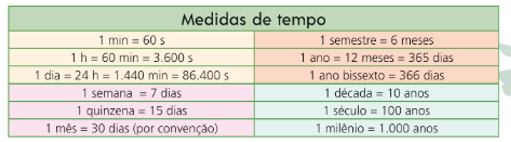
\includegraphics[width=4.25870in,height=1.18344in]{media/image40.png}}

\colorsec{Atividades}

\num{1}

Veja a imagem de uma fita métrica. Ela é utilizada para medir
comprimento.

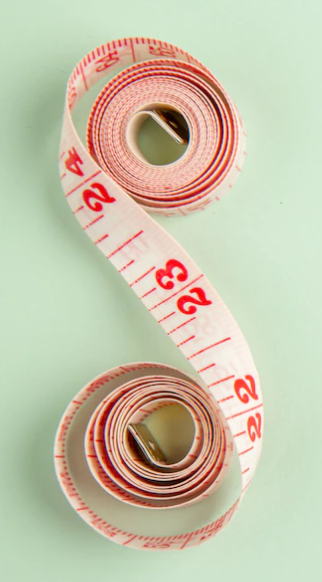
\includegraphics[width=1.29167in,height=2.33463in]{media/image41.png}

\url{https://img.freepik.com/fotos-gratis/vista-superior-centimetro-rosa-sobre-fundo-verde_179666-22646.jpg?w=1060\&t=st=1677438557~exp=1677439157~hmac=a65357a78e180ff6d1282de8980ca1bfdad02d17329ce5b2620459dcac61e3b8}

\begin{escolha}

\item
  Escreva o nome de dois objetos de sua sala de aula que você acredita
  medir menos que 1 metro.
\linhas{2}
\coment{Resposta pessoal}

\item
  Escreva o nome de dois objetos de sua sala de aula que você acredita
  medir mais que 1 metro.
\linhas{2}
\coment{Resposta pessoal}

\end{escolha}

\num{2}

Utilize sua régua e responda aos itens abaixo:

\begin{escolha}

\item
  Quantos centímetros tem o comprimento de sua borracha?
\linhas{2}
\coment{Resposta pessoal.}

\item
  Qual a largura, em centímetros, da carteira que você utiliza em sua
  sala de aula?
\linhas{2}
\coment{Resposta pessoal.}

\item
  Qual o comprimento, em centímetros, de seu lápis?
\linhas{2}
\coment{Resposta pessoal.}

\item
  Qual a altura aproximada de um de seus colegas?
\linhas{2}
\coment{Resposta pessoal.}

\end{escolha}

\num{3}

Relacione a primeira com a segunda coluna levando em conta qual valor
pode corresponder a medida que é mostrada.

\begin{escolha}

\item
  Altura aproximada de uma porta ( )20 cm
\item
  Comprimento aproximado de um lápis ( ) 90 m
\item
  Comprimento médio de um quarteirão ( ) 30 m
\item
  Comprimento aproximado de uma quadra de basquete ( ) 2 m

\end{escolha}

Resposta:

A = 2 m

B = 20 cm

C = 90 m

D = 30 m

\coment{Explore bastante com os alunos esse senso de tamanho pois esse
é um conceito extremamente importante para eles.}

\num{4}

Complete a frase com o número que representa quanto mede cada um dos
objetos indicados a seguir.

\begin{escolha}

\item
  O lápis abaixo mede -\/-\/-\/-9-\/-\/-\/-\/-\/-\/- cm.

  
\includegraphics[width=4.00868in,height=0.70839in]{media/image42.png}

  O lápis na régua deve sair exatamente do 0 e chegar exatamente no 9.


\item
  A borracha abaixo mede -\/-\/-\/-6-\/-\/-\/-\/- cm

  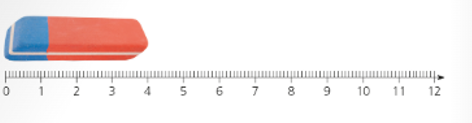
\includegraphics[width=3.93367in,height=1.02509in]{media/image43.png}

  A borracha deve sair exatamente do zero e chegar exatamente no 6.

\item
  O apontador abaixo mede -\/-\/-\/-\/-4-\/-\/-\/-\/-cm

  
\includegraphics[width=3.87534in,height=0.95842in]{media/image44.png}

  O apontador deve começar exatamente no 3 e terminar exatamente no 7.

\item
  A tesoura abaixo mede -\/-\/-\/-10-\/-\/-\/-cm

  \begin{quote}
  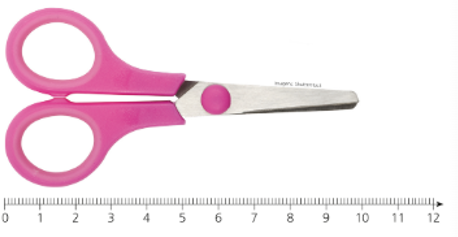
\includegraphics[width=3.81700in,height=1.97517in]{media/image45.png}
\end{quote}

  Deixar um pedaço de linha nos locais indicados por traços nos itens
acima.

  A tesoura deve sair exatamente do 1 e chegar exatamente no 11
\end{escolha}

\coment{Professor explore bastante essa questão de medir com o auxílio da reta
numérica, principalmente quando o início não é no zero. Esse conceito é
muito útil para entendimento de assuntos que virão em outros anos e
trabalhar bastante agora pode facilitar a vida do aluno em anos
posteriores.}

\num{5}

Debora decidiu estimar a medida do lápis com sua borracha.

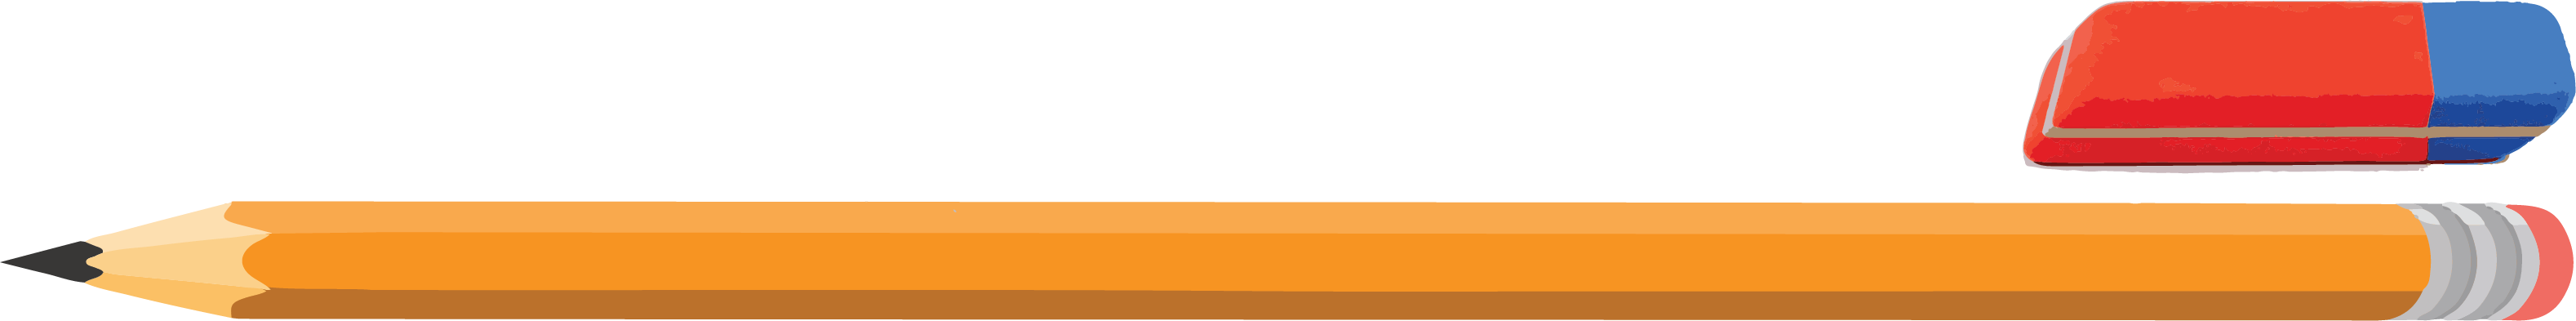
\includegraphics[width=3.84200in,height=1.23344in]{media/image46.png}

O lápis e a borracha devem ter tamanhos de forma que no comprimento de
um lápis caibam de 4 a 5 borrachas. O desenho é fundamental para a
resolução dessa questão.

Quantas borrachas, considerando a figura dada, aproximadamente, mede o
lápis de Debora?

\begin{escolha}
\item
  Entre 2 e 3.
\item
  Entre 4 e 5
\item
  Entre 6 e 7
\item
  Mais que 9
\end{escolha}

Resposta: B

Através da percepção de comparação de comprimentos, percebe-se que no
comprimento de um lápis cabem cerca de 4 a 5 borrachas conforme a figura
dada.

\num{6}

Um dos brinquedos do parque de diversões permanente de uma cidade proíbe
que crianças com uma altura menor que 1,30 m possam brincar nessa
atração. Manoel mediu sua altura e ele está com 93 cm. Quanto ele
precisa crescer para poder realizar seu sonho de andar nesse brinquedo?

Deixar espaço em branco equivalente a 2 linhas para cálculos

Resposta:

1,20 m = 130 cm

130 -- 93 = 33 cm

Portanto ele ainda precisará crescer 33 cm para que esteja apto a andar
nesse brinquedo.

\num{7}

Roberto está com sintomas de dor de garganta e sua mãe o levou ao
médico. Chegando lá sua temperatura foi medida e a foto do termômetro
está abaixo.

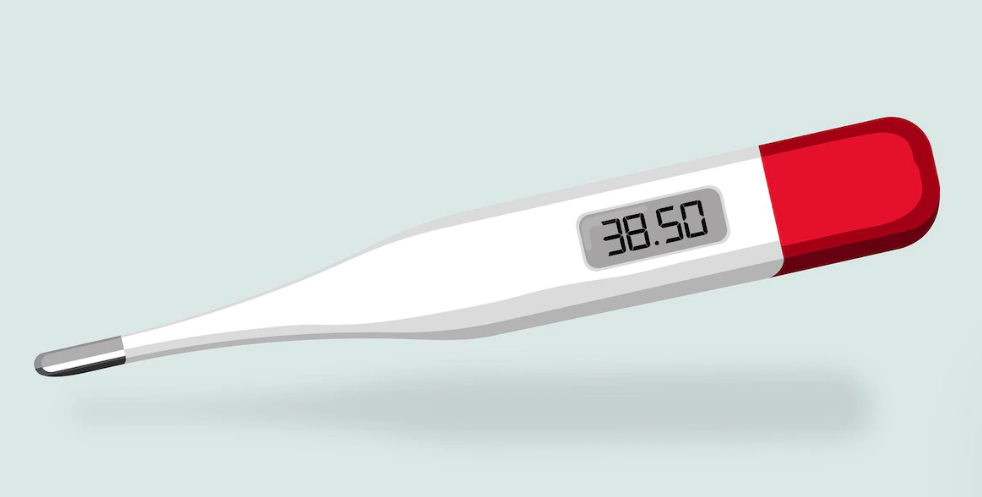
\includegraphics[width=3.15000in,height=1.59426in]{media/image47.png}

\url{https://img.freepik.com/vetores-gratis/elemento-termometro-digital-38-5-graus-celsius_53876-119949.jpg?w=1380\&t=st=1677436599~exp=1677437199~hmac=efddbcbdae2d4d75bd1e8476eee389a985a191d57800533acdff847111e69669}

A temperatura indicada no termômetro deve ser de 39,5º C

Analisando a imagem do termômetro podemos concluir que a temperatura de
Roberto nesse instante era de:

\begin{escolha}

\item
  38,5º C
\item
  39ºC
\item
  39,5º C
\item
  40º
\end{escolha}

Resposta: C

Observando a figura percebemos que o termômetro está marcando exatamente
39,5ºC

\num{8}

Para a festa de aniversário de Arthur, seu pai encomendou 24 garrafas de
refrigerante. Dessas garrafas, 10 continham, cada uma, 3 litros. Nas
demais garrafas, havia dois litros em cada uma. Com base nessas
informações responda ao que se pede:

\begin{escolha}

\item
  Qual a quantidade, em mililitros, encomendada pelo pai de Arthur?
\linhas{3}
\coment{(10 x 3) + (14 x 2) = 30 + 28 = 58 l = 58 000 ml}

\item
  Se cada pessoa consumiu exatamente 400 mililitros de refrigerante e
  todo o refrigerante foi consumido durante a festa, quantas pessoas
  foram ao aniversário de Arthur?
\linhas{3}
\coment{58 000 : 400 = 145 pessoas compareceram a festa.}

\end{escolha}

\num{9}

O comprimento de uma escrivaninha é de 1,6 m. Quantos palmos,
aproximadamente, mede a escrivaninha se, em média, um palmo tem 23 cm?

\begin{escolha}

\item
  5 palmos
\item
  6 palmos
\item
  7 palmos
\item
  8 palmos
\end{escolha}

Resposta: C

1,6 m = 160 cm

160 : 23 = 6,95 palmos. Aproximadamente 7 palmos.

\num{10}

Uma série de televisão proporciona episódios com duração de 45 minutos.
Se Jorge terminou de assistir esse episódio as 17 horas, qual foi o
horário que ele começou a assistir esse episódio se ele assistiu no
início ao fim sem parar nenhuma vez?

Deixar espaço em branco equivalente a 2 linhas para cálculos

Resposta:

Ele começou a assistir o episódio às 16 horas e 15 minutos pois se nesse
horário somarmos a duração do episódio, que é de 45 minutos, teremos o
horário final que foi 17 horas.

\colorsec{Treino}

\num{1}

Reinaldo foi contratado por uma empresa que possui um horário bem rígido
e semanal que deve ser cumprido corretamente. No período da manhã e deve
cumprir 4 horas e 30 minutos de trabalho. Qual será o horário que
Reinaldo saíra para almoçar?

\begin{longtable}[]{@{}lll@{}}
\toprule
& Entrada & Saída\tabularnewline
\midrule
\endhead
Manhã & 8:00 & ?\tabularnewline
Tarde & 14:00 & 17:30\tabularnewline
\bottomrule
\end{longtable}

\begin{escolha}
\item
  11h00
\item
  11h30
\item
  12h00
\item
  12h30
\end{escolha}

Resposta: D

Como pela manhã ele entra as 8:00 e deve cumprir nesse período 4 horas e
meia de trabalho antes de sair para o almoço, conclui-se que ele saíra
para o almoço às 12:30.

\num{2}

Na receita médica de Marcela recomenda que ela tome um xarope 3 vezes ao
dia e que cada vez ela tome a quantidade de 10 ml durante 7 dias. Um
frasco do remédio contém 100 ml. Sendo assim, qual a quantidade de
frascos que a mãe de Marcela terá que comprar para que todo tratamento
seja concluído?

\begin{escolha}

\item
  1
\item
  2
\item
  3
\item
  4
\end{escolha}

Resposta: C

3 x 10 x 7 = 210 ml. Como cada frasco possui 100 ml, ela terá que
comprar 3 frascos e haverá uma sobra de xarope.

\num{3}

Vicente teve que fazer uma viagem para fechar um grande negócio. Se vôo
saiu do aeroporto as 10 horas e 42 minutos e chegou ao seu destino às 14
horas e 8 minutos. Qual foi o tempo de duração do vôo?

\begin{escolha}

\item
  3 horas e 16 minutos
\item
  2 horas segundos
\item
  2 horas e 42 minutos
\item
  3 horas e 58 minutos
\end{escolha}

Resposta: A

Saída: 10 horas e 42 minutos

Chegada: 14 horas e 8 minutos

Tempo de vôo: 3 horas e 16 minutos = 196 minutos = 3 horas e 16 minutos

\chapter{}
\markboth{Módulo 5}{}

\coment{Habilidades da BNCC: EF03MA22, EF03MA23}

\colorsec{Habilidades do SAEB}

\begin{itemize}
    \item Medir ou comparar perímetro ou área de figuras planas desenhadas em
malha quadriculada.

    \item Identificar horas em relógios analógicos ou associar horas em relógios
analógicos e digitais.

    \item Resolver problemas que envolvam perímetro de figuras planas.

    \item Resolver problemas que envolvam área de figuras planas.
\end{itemize}

\conteudo{

Semana: Uma semana é composta por 7 dias e os dias da semana estão na
tabela abaixo:

\begin{longtable}[]{@{}l@{}}
\toprule
Dias da semana\tabularnewline
\midrule
\endhead
Domingo\tabularnewline
Segunda-feira\tabularnewline
Terça-feira\tabularnewline
Quarta-feira\tabularnewline
Quinta-feira\tabularnewline
Sexta-feira\tabularnewline
Sábado\tabularnewline
\bottomrule
\end{longtable}

Ano: O ano é composto por 12 meses. O nome dos meses e as suas
respectivas quantidades de dias estão na tabela abaixo:

\begin{longtable}[]{@{}ll@{}}
\toprule
Meses que compõem o ano & Número de dias dos meses\tabularnewline
\midrule
\endhead
Janeiro & 31\tabularnewline
Fevereiro & 28 (no ano bissexto terá 29 dias)\tabularnewline
Março & 31\tabularnewline
Abril & 30\tabularnewline
Maio & 31\tabularnewline
Junho & 30\tabularnewline
Julho & 31\tabularnewline
Agosto & 31\tabularnewline
Setembro & 30\tabularnewline
Outubro & 31\tabularnewline
Novembro & 30\tabularnewline
Dezembro & 31\tabularnewline
\bottomrule
\end{longtable}

Relógio Analógico:

Como é dividido: O relógio de ponteiro é dividido em 12 partes ou
seções. Você pode reparar que da esquerda para a direita o acessório é
numerado de 1 a 12. Esses números representam as horas.

Por sua vez, o intervalo de tempo que fica entre cada um deles
representa a contagem dos minutos. Assim, ficou convencionado que~o
intervalo entre cada um deles é de 5 minutos. Então, a partir do número,
você precisa adicionar 5 minutos a cada número.

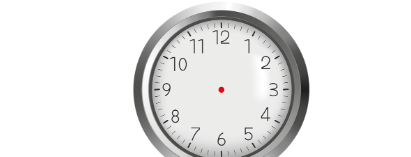
\includegraphics[width=2.95833in,height=1.13007in]{media/image48.png}

Ordem de leitura dos ponteiros do relógio analógico: a leitura dos
ponteiros do relógio começa sempre pelas horas. Depois, minutos e
segundos.

Utilização dos ponteiros para efetuar a leitura:

\begin{itemize}
\item
  o ponteiro menor é o primeiro que você deve observar. Por exemplo, se
  o ponteiro menor estiver sobre ou próximo do 7, indica que são sete
  horas.
\end{itemize}

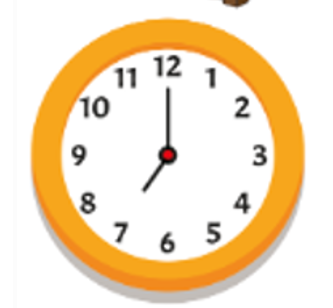
\includegraphics[width=1.69271in,height=1.56563in]{media/image49.png}

\begin{itemize}
\item
  Use o ponteiro maior para ler os minutos: o ponteiro maior marca os
  minutos, dessa forma, se ele estiver parado sobre o 6, significa que
  30 minutos já se passaram.
\end{itemize}

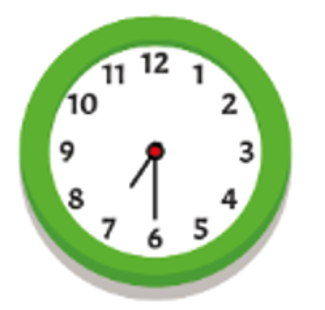
\includegraphics[width=1.57292in,height=1.50032in]{media/image50.png}

Em seguida para saber as horas junte as duas informações apresentadas
acima:

\begin{itemize}
\item
  Ponteiro menor perto do 7
\item
  Ponteiro maior em cima do 6 (30 minutos)
\end{itemize}

Portanto, iremos ler 7 horas e 30 minutos.}

\colorsec{Atividades}

\num{1}

Observe os horários nos relógios representados abaixo

Produzir imagem desses relógios com as respectivas horas indicadas

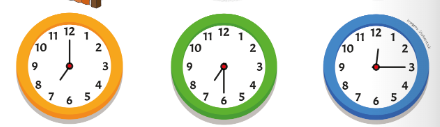
\includegraphics[width=3.66698in,height=1.05843in]{media/image51.png}

Qual o horário cada relógio está marcando?

\linhas{3}
\coment{Primeiro relógio: sete horas
Segundo relógio: sete horas e trinta minutos (sete e meia)
Terceiro relógio: doze horas e quinze minutos (meio dia e quinze)}

\num{2}

Observe o horário que os relógios digitais estão marcando:

Produzir imagem de relógios digitais com essas horas

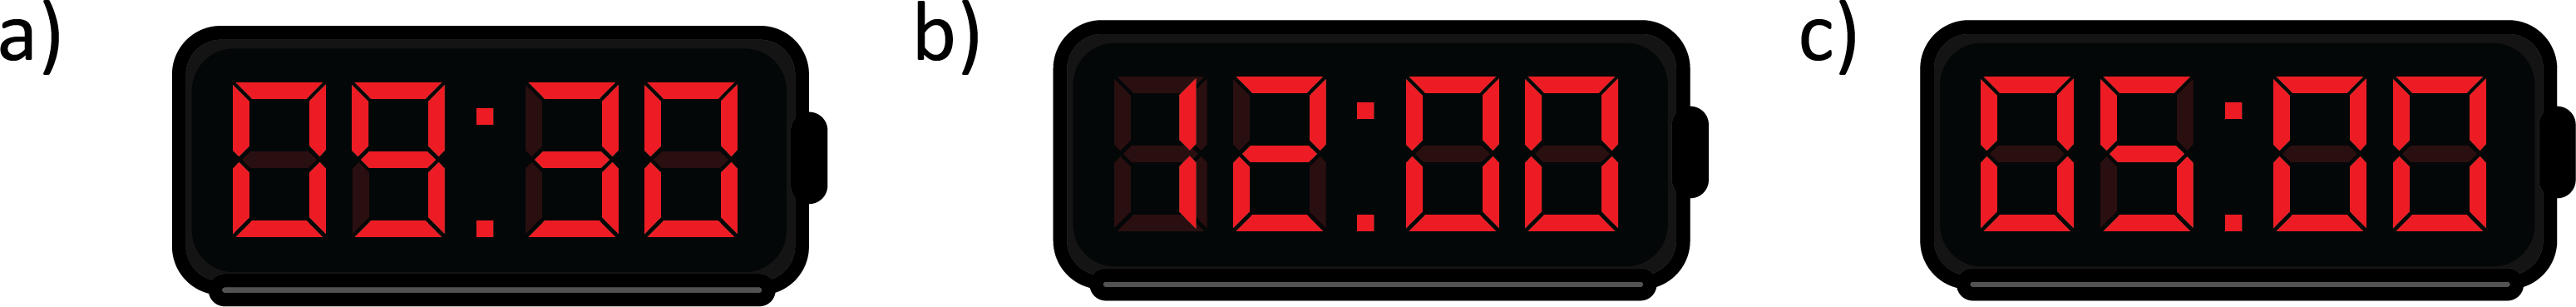
\includegraphics[width=3.54197in,height=0.29169in]{media/image52.png}

Como se lê cada um dos horários marcados?

\linhas{4}
\coment{

\begin{escolha}
\item
  Nove e meia ou nove horas e trinta minutos
\item
  Meio dia ou doze horas
\item
  Cinco horas
\end{escolha}}

\num{3}

A professora de Francisco colocou com primeira questão da prova a
seguinte imagem:

Produzir uma imagem como essa

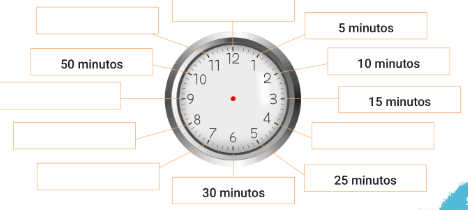
\includegraphics[width=3.90034in,height=1.75015in]{media/image53.png}

Ajude Francisco a completar os retângulos em branco com indicação de
minutos que cada um deles aponta.

Resposta:

Vinte minutos; 35 minutos; 40 minutos; 45 minutos; 55 minutos; 60
minutos

\num{4}

Observe o calendário abaixo e em seguida responda aos itens propostos.

Colocar uma imagem de calendário conforme essa abaixo.

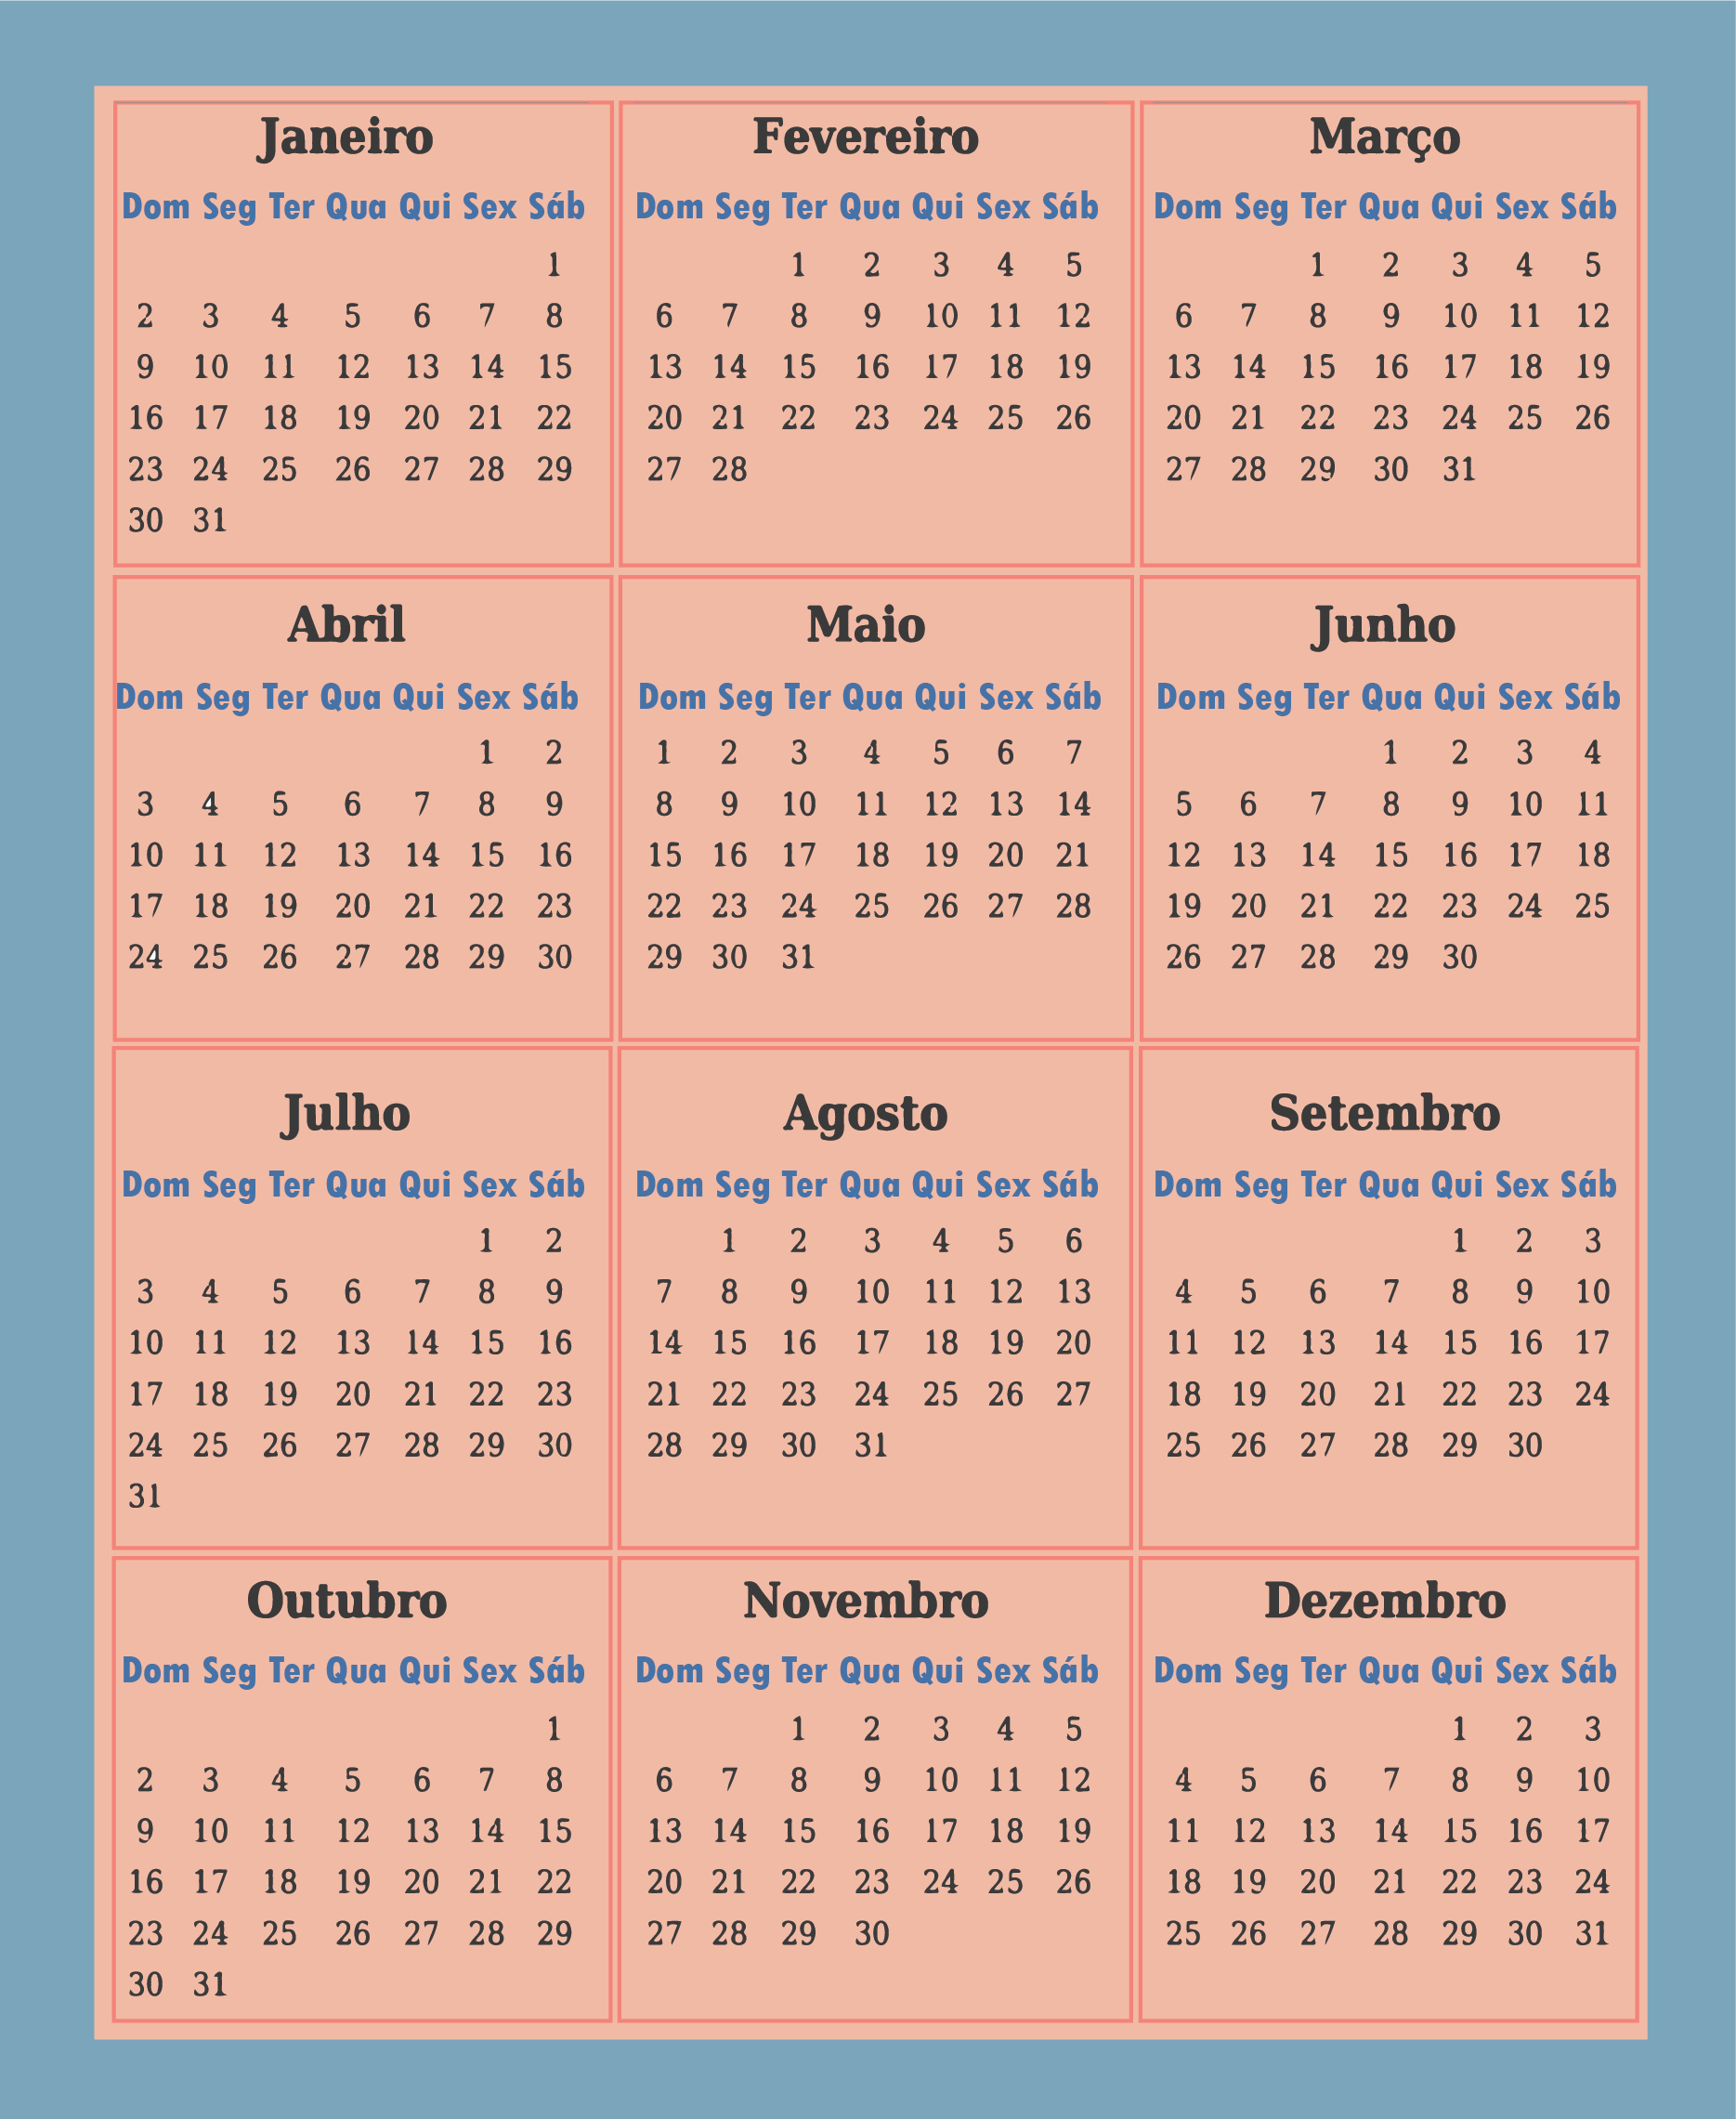
\includegraphics[width=4.13369in,height=3.20861in]{media/image54.png}

\begin{escolha}
\item
  Circule no calendário o dia de seu aniversário.
  \coment{Resposta pessoal.}

\item
  Agora, com um retângulo marque o dia do aniversário de três
  coleguinhas da sua sala.
  \coment{Resposta pessoal.}

\item
  Marque com um triângulo o dia do aniversário de seu professor.
  \coment{Resposta pessoal.}

\item
  Quantos anos você tem?
  \linhas{1}
  \coment{Resposta pessoal.}

\item
  Você tem mais ou menos de 450 meses?
  \linhas{4}
  \coment{Resposta pessoal.}
\end{escolha}

\num{5}

Complete o quadro abaixo com o auxílio de colegas e de seu professor.

\begin{longtable}[]{@{}ll@{}}
\toprule
Meses que compõem um ano & Número de dias que esse mês
possui\tabularnewline
\midrule
\endhead
Janeiro &\tabularnewline
Fevereiro &\tabularnewline
Março &\tabularnewline
Abril &\tabularnewline
Maio &\tabularnewline
Junho &\tabularnewline
Julho &\tabularnewline
Agosto &\tabularnewline
Setembro &\tabularnewline
Outubro &\tabularnewline
Novembro &\tabularnewline
Dezembro &\tabularnewline
\bottomrule
\end{longtable}

Resposta:

\begin{longtable}[]{@{}ll@{}}
\toprule
Meses que compõem um ano & Número de dias que esse mês
possui\tabularnewline
\midrule
\endhead
Janeiro & 31\tabularnewline
Fevereiro & 28 (no ano bissexto 29)\tabularnewline
Março & 31\tabularnewline
Abril & 30\tabularnewline
Maio & 31\tabularnewline
Junho & 30\tabularnewline
Julho & 31\tabularnewline
Agosto & 31\tabularnewline
Setembro & 30\tabularnewline
Outubro & 31\tabularnewline
Novembro & 30\tabularnewline
Dezembro & 31\tabularnewline
\bottomrule
\end{longtable}

\num{6}

O pai de Rafael estava conversando com um contador sobre o seu
faturamento semestral. Rafael escutou toda conversa e depois fez os
seguintes questionamentos a seu pai. Pai o que um semestre? Quantos
meses compõem um semestre? Quanto semestre temos em um ano?

Diante de tantas perguntas o pai de Rafael sentou-se com seu filho e
começou a responder aos questionamentos do filho.

Ajude o pai de Rafael a responder corretamente todas as perguntas que o
filho lhe fez.

Deixar espaço de 5 linhas para a resposta

Resposta:

Um semestre é um período composto por 6 meses e em um ano temos 2
semestres.

\num{7}

Marque desenhando no relógio analógico abaixo os ponteiros das horas e
minutos na posição exata que estarão para representar o horário em que
suas aulas começam.

Faça uma figura semelhante a abaixo sem os ponteiros.

\includegraphics[width=3.42530in,height=1.30845in]{media/image48.png}

Resposta

Resposta pessoal, mas professor debata com os alunos qual é o ponteiro
das horas e qual o dos minutos e comece a introduzir velocidade só
comentando quanto tempo cada um demora para percorrer uma certa região
do relógio

\num{8}

Renato aos finais de semana anda de bicicleta ao redor da praça
existente no bairro em que mora.

Produzir uma imagem semelhante a abaixo

\includegraphics[width=2.35256in,height=2.20730in]{media/image55.png}

Se ele der duas voltas completas ao redor da praça, ele percorrerá qual
distância?

Deixar espaço em branco equivalente a duas linhas para cálculos

Resposta:

(2 x 30 + 2 x 50) x 2 = 320 m

Professor sempre que possível estimule a montagem da expressão para que
os alunos comecem a se acostumar.

\num{9}

As figuras abaixo foram desenhadas em uma malha quadriculada.

Produzir uma imagem semelhante a abaixo

Cores importam

\includegraphics[width=2.59189in,height=1.55847in]{media/image56.png}

Quantos quadradinhos pintados cada figura possui?

Deixar espaço de 3 linhas para a resposta

Resposta:

Verde: 21 quadradinhos

Azul: 24 quadradinhos

Laranja: 9 quadradinhos

\num{10}

Os desenhos representados abaixo foram feitos com o auxílio de uma malha
quadriculada na qual cada lado do quadradinho mede 1 cm.

Produzir uma imagem semelhante a abaixo. Cores importam

\includegraphics[width=2.47521in,height=1.77515in]{media/image57.png}

\begin{escolha}

\item
  Qual a medida, em centímetros, do contorno da figura azul?
\linhas{1}
\coment{18 cm}

\item
  Qual a medida, em centímetros, do contorno da figura amarela?
\linhas{1}
\coment{12 cm}

\item
  Qual a medida, em centímetros, do contorno da figura verde?
\linhas{1}
\coment{22 cm}

\end{escolha}

\num{11}

Utilizando sua régua uma pontos e faça uma figura na malha quadriculada
abaixo representada apenas pelos pontinhos. Em seguida, mostra sua
figura para um colega e veja se ele descobre o que você representou.

Produzir uma imagem semelhante a abaixo

\includegraphics[width=4.05869in,height=1.93350in]{media/image58.png}

Resposta:

Resposta pessoal.

\num{12}

Observe atentamente as figuras abaixo:

Produzir uma imagem semelhante a abaixo sem os escritos

\includegraphics[width=3.72532in,height=2.47521in]{media/image59.png}

Quais delas possuem a mesma quantidade de quadradinhos? Justifique sua
resposta.

Deixar espaço de 1 linha para a resposta

Resposta:

Todas são compostas pelo mesmo número de quadradinhos.

\num{13}

Na malha quadriculada abaixo, cada quadrado representa uma área de 10
metros quadrados.

Produzir uma imagem semelhante a abaixo

\includegraphics[width=3.33333in,height=1.50517in]{media/image60.png}

Qual a área da malha quadriculada que a figura destacada ocupa?

Deixar espaço de 3 linhas para a resposta

Resposta:

Realizando a contagem de quadradinhos que preenchem a figura chega-se
que para o preenchimento dela são necessários 16 quadradinhos.

Portanto, 16 x 10 = 160 metros quadrados.

\colorsec{Treino}

\num{1}

Paulo resolveu ir a uma exposição e no momento se encontra na
bilheteria. Quanto ele precisará andar para chegar à exposição,
considerando o caminho destacado, sabendo-se que o lado de cada
quadradinho da malha tem medida de 3m?

Produzir uma imagem conforme abaixo

\includegraphics[width=2.60897in,height=1.46587in]{media/image61.png}

\begin{escolha}
\item
  5 m
\item
  10 m
\item
  12 m
\item
  15 m
\end{escolha}

Resposta: D

Ele deverá andar 5 lados de quadrado. Como cada lado de quadrado possui
medida igual a 3 m, ele deverá andar 15 metros.

\num{2}

Leandro resolveu cobrir de azuleijos a fundo de sua piscina de tal forma
que apareça, no fundo, a letra inicial do nome de seu filho Arnaldo.
Sabendo-se que cada quadradinho corresponde a um azuleijo, quantos
azuleijos foram utilizados para cobrir a letra inicial do nome de seu
filho?

Produzir uma imagem semelhante a abaixo

\includegraphics[width=1.42949in,height=1.25160in]{media/image62.png}

\begin{escolha}
\item
  13
\item
  14
\item
  16
\item
  20
\end{escolha}

Resposta: B

Realizando a contagem do número de quadradinhos que formam a letra A
percebemos que são 14 quadradinhos.

\num{3}

Os desenhos representados abaixo representam as plantas baixas, inicial
e final, e o formato de uma praça que será construída em uma área
central de uma cidade. Inicialmente a previsão era para uma praça
pequena, mas como a prefeitura conseguiu uma área maior ao lado da
primeira resolveu-se realizar a construção de uma praça maior.

Produzir uma imagem semelhante a abaixo

\includegraphics[width=5.00877in,height=1.80849in]{media/image63.png}

Sendo assim, a nova praça terá uma área com relação a praça que se
desejava construir iniciamente:

\begin{escolha}
\item
  2 vezes maior
\item
  3 vezes maior
\item
  4 vezes maior
\item
  5 vezes maior
\end{escolha}

Resposta: C

A praça menor teria 6 quadradinhos preenchendo sua área enquanto a
grande terá 24 quadradinhos e sendo assim, a área da praça maior e
quatro vezes a área da praça menor.

\chapter{}
\markboth{Módulo 6}{}

\coment{Habilidades da BNCC: EF03MA24}

\colorsec{Habilidades do SAEB}

\begin{itemize}
    \item Relacionar valores de moedas e/ou cédulas do sistema monetário
brasileiro, com base nas imagens desses objetos.

    \item Resolver problemas que envolvam moedas e/ou cédulas do sistema
monetário brasileiro.
\end{itemize}

\conteudo{

\coment{Professor talvez esse módulo está entre os principais. É muito
importante que os alunos comecem a entender como lidar com o dinheiro.
Explore ao máximo as atividades além de outras situações que podem
despertar o interesse e promover um início da educação e conscientização
financeira.}

Conhecendo nosso dinheiro

\includegraphics[width=1.80833in,height=1.75637in]{media/image64.png}Moeda
de 5 centavos: R\$ 0,05

\url{https://img.freepik.com/fotos-gratis/dinheiro-moedas-brasileiras-5-centavos_58702-6209.jpg?w=1060\&t=st=1677437125~exp=1677437725~hmac=c640dd9c5a2963fb4f314f44e074b714cda9416e178bd281b3d494e8262ac50e}

\includegraphics[width=1.50833in,height=1.45668in]{media/image65.png}Moeda
de 10 centavos: R\$ 0,10

\includegraphics[width=1.52500in,height=1.24749in]{media/image66.png}Moeda
de 25 centavos: R\$ 0,25

\url{https://img.freepik.com/fotos-gratis/dinheiro-moedas-brasileiras-25-centavos_58702-6230.jpg?w=1060\&t=st=1677437194~exp=1677437794~hmac=db98c5063a731e98b23627749d52c094bab4a2f113240f1f248ee1be7074b235}

\includegraphics[width=1.56667in,height=1.61849in]{media/image67.png}Moeda
de 50 centavos: R\$ 0,50

\url{https://img.freepik.com/fotos-gratis/dinheiro-moedas-brasileiras-50-centavos_58702-6291.jpg?w=1060\&t=st=1677437366~exp=1677437966~hmac=a914e13013ee69679658ce52473a57d18d6d23ed6356e75e5d5a34316e88cd82}

\includegraphics[width=2.11667in,height=2.01180in]{media/image68.png}Moeda
de 1 real: R\$ 1,00.

\url{https://img.freepik.com/fotos-gratis/dinheiro-moedas-brasileiras-1-real_58702-6210.jpg?w=1060\&t=st=1677437258~exp=1677437858~hmac=3314b729d5619da0bffa3b7ce7fe354ae155c324f94ca82e2cb356693ffc25dc}

\includegraphics[width=2.71068in,height=1.97500in]{media/image69.png}Ao
lado de cada nota colocar: Nota de 2 reais: R\$ 2,00; Nota de 5 reais
R\$ 5,00; Nota de 10 reais: R\$ 10,00; Nota de 20 reais: R\$ 20,00. Nota
de 50 reais: R\$ 50,00

\url{https://img.freepik.com/vetores-gratis/ilustracao-gradiente-de-caixa-brasileira_52683-78831.jpg?w=996\&t=st=1677437712~exp=1677438312~hmac=c23ec28122c2591b7b261ceca09eb7c0a64059387f9729dc642986ca98524f1c}
n

\includegraphics[width=3.18285in,height=1.50833in]{media/image70.png}Nota
de 100 reais R\$ 100,00

\url{https://img.freepik.com/fotos-premium/cem-reais-contas-dinheiro-brasileiro_499484-1535.jpg?w=1060}

\includegraphics[width=2.68333in,height=1.88913in]{media/image71.png}Nota
de 200 reais: R\$ 200,00}

\colorsec{Atividades}

\num{1}

Complete o quadro abaixo relacionando a imagem das cédulas e moedas do
sistema monetário brasileiro com seu valor e como se lê.

Colocar no espaço da cédula ou moeda a foto das seguinte nota

\begin{longtable}[]{@{}lll@{}}
\toprule
Cédula ou moeda & Valor & Como se lê\tabularnewline
\midrule
\endhead
Foto nota 200 reais & & Duzentos reais\tabularnewline
Foto nota 100 reais & &\tabularnewline
Foto nota 50 reais & &\tabularnewline
Foto de 20 reais & R\$ 20,00 &\tabularnewline
Foto de 10 reais & &\tabularnewline
Foto de 5 reais & & Cinco reais\tabularnewline
Foto nota 2 reais & &\tabularnewline
Foto moeda de 1 real & &\tabularnewline
Foto moeda de 0,50 centavos & R\$ 0,50 &\tabularnewline
Foto moeda de 0,25 centavos & &\tabularnewline
Foto moeda de 0,10 centavos & &\tabularnewline
Foto moeda de 0,05 centavos & & Cinco centavos\tabularnewline
\bottomrule
\end{longtable}

Resposta:

monetário brasileiro com seu valor e como se lê.

Colocar no espaço da cédula ou moeda a foto das seguintes nota

\begin{longtable}[]{@{}lll@{}}
\toprule
Cédula ou moeda & Valor & Como se lê\tabularnewline
\midrule
\endhead
Foto nota 200 reais & R\$ 200,00 & Duzentos reais\tabularnewline
Foto nota 100 reais & R\$ 100,00 & Cem reais\tabularnewline
Foto nota 50 reais & R\$ 50,00 & Cinquenta reais\tabularnewline
Foto de 20 reais & R\$ 20,00 & Vinte reais\tabularnewline
Foto de 10 reais & R\$ 10,00 & Dez reais\tabularnewline
Foto de 5 reais & R\$ 10,00 & Cinco reais\tabularnewline
Foto nota 2 reais & R\$ 2,00 & Dois reais\tabularnewline
Foto moeda de 1 real & R\$ 1,00 & Um real\tabularnewline
Foto moeda de 0,50 centavos & R\$ 0,50 & Cinquenta
centavos\tabularnewline
Foto moeda de 0,25 centavos & R\$ 0,25 & Vinte e cinco
centavos\tabularnewline
Foto moeda de 0,10 centavos & R\$ 0,10 & Dez centavos\tabularnewline
Foto moeda de 0,05 centavos & R\$0,05 & Cinco centavos\tabularnewline
\bottomrule
\end{longtable}

\num{2}

André foi ao banco efetuar um saque (retirada de dinheiro de sua conta
bancária) e ao pegar o valor pretendido recebeu as seguintes cédulas e
moedas:

Produzir uma figura conforme a abaixo mantendo as quantidades das notas

\includegraphics[width=2.50022in,height=1.34178in]{media/image72.png}
\includegraphics[width=2.26686in,height=0.87508in]{media/image73.png}

Qual o valor que André retirou de sua conta bancária:

Deixar espaço de 3 linhas para a resposta

Resposta:

1 x 50 + 4 x 20 + 1 x 10 + 3 x 5 + 2 x 2 + 2 x 1 + 4 x 0,50 = 50 + 80 +
10 + 15 + 4 + 2 + 2 = R\$ 173,00.

\num{3}

A mãe de Leonardo foi a supermercado e comprou os seguintes produtos:

Produzir uma imagem como a abaixo mantendo valores e quantidades

\includegraphics[width=4.10036in,height=1.22511in]{media/image74.png}

Observando o preço pago por cada produto e a quantidade que ela comprou
de cada um, pode-se afirmar que o gasto dela no supermercado foi igual
a:

\begin{escolha}

\item
  R\$ 35,00
\item
  R\$ 42,00
\item
  R\$ 61,00
\item
  R\$ 67,00
\end{escolha}

Resposta: D

Açúcar: R\$: 5,00

Suco: 3 x 3 = R\$ 9,00

Arroz: R\$ 10,00

Queijo: 19,00

Manteiga: R\$ 15,00

Café: R\$ 9,00

Valor total: 5 + 9 + 10 + 19 + 15 + 9 = R\$ 67,00

\num{4}

Um grande rede de lojas realizou uma promoção de vendas após o Natal.
Veja os produtos que estava em promoção e seus respectivos preços:

Produzir uma imagem como abaixo mantendo os valores

\includegraphics[width=3.30029in,height=1.97517in]{media/image75.png}

Observavdo a figura, resposda a cada item:

\begin{escolha}

\item
  Se uma pessoa comprar um fogão e um liquidificador quanto irá pagar?
\linhas{3}
\coment{1 300 + 250 = R\$ 1 550,00}

\item
  Se uma pessoa conseguir um desconto de R\$ 50,00 para pagamento a
  vista na compra do micro-ondas, qual será o valor que ela pagará?
\linhas{3}
\coment{480 -- 50 = R\$ 430,00}

\end{escolha}

\num{5}

A tabela a seguir mostra a pesquisa de preços que José está fazendo
sobre Um jogo de vídeo game e um controlo bluetooth:

\begin{longtable}[]{@{}lll@{}}
\toprule
Produto & Loja A & Loja B\tabularnewline
\midrule
\endhead
Jogo de vídeo game & R\$ 200,00 & R\$ 176,00\tabularnewline
Controle bluetooth & R\$ 616,00 & R\$ 654,00\tabularnewline
total & &\tabularnewline
\bottomrule
\end{longtable}

\begin{escolha}

\item
  Se ele comprar os dois itens na loja A pagará quanto?
\linhas{3}
\coment{200 + 616 = R\$ 816,00}

\item
  Se optar comprar tuda na loja B qual o valor que ele pagará?
\linhas{3}
\coment{176 + 654 = R\$ 830,00}

\item
  Se ele quer pagar o menor preço possível, determine em qual loja ele
  deverá comprar cada item e qual o valor que pagará.
\linhas{3}
\coment{Ele deverá comprar o jogo na loja B por R\$ 176,00 e o controle na
  loja A por R\$ 616,00. Com isso pagará R\$ 792,00.}
\end{escolha}

\num{6}

Marta foi a papelaria comprar uma caneta que estava precisando para
continuar seus estudos. Ela comprou uma caneta que custava 7 reais e 75
centavos. Sabendo-se que ela pagou com uma nota de 10 reais, quais
cédulas e moedas ela recebeu de troco?

\linhas{2}
\coment{Como o enunciado estimula que são cédulas e moedas ela deva ter recebido
de troco uma nota de 2 reais e 1 moeda de 25 centavos.
Existem outras opções, explore as outras combinações com seus alunos.
Explorar com os alunos outras situações para que treinem um
pouco esse conceito. Além disso, converse um pouco com os alunos sobre
outras moedas que existem no mundo e qual o seu valor em relação ao real
e vice e versa.}

\num{7}

Caique economizou muito dinheiro pois queria comprar um vídeo game usado
que custava R\$ 3 490,00 à vista. Ele conversou com o vendedor e pediu
um desconto extra e foi atendido com um desconto de R\$ 350,00. Quanto
ele pagou pelo vídeo game?

Deixar espaço em branco equivalente a 3 linhas para a resolução

Resposta:

R\$ 3 490,00 -- R\$ 350,00 = R\$ 3 140,00

\num{8}

Em muitas compras a prazo e exigido uma entrada que é paga no ato da
compra e o restante do valor pode ser dividido em um número combinado de
parcelas mensais. Veja o exemplo exibido abaixo.

\includegraphics[width=2.90025in,height=0.89174in]{media/image76.png}

Produzir uma imagem como acima. O escrito deve ser: Entrada R\$ 25 000,00
e o restante dividido em 36 parcelas de R\$ 1 200,00 cada uma.

\begin{escolha}

\item
  Qual o valor que será dividido em 24 vezes?
\linhas{3}
\coment{24 x 1 200 = R\$ 28 800,00}

\item
  Qual o valor que cada parcela terá?
\linhas{3}
\coment{Lendo atentamente o texto sabe-se que será de R\$ 1 200,00}

\item
  Se à vista a loja fornece um desconto de R\$ 2 580,00, que optar por
  pagar à vista pagará quanto pelo carro?
\linhas{3}
\coment{25 000 + (24 x 1 200) -- 2 580 = R\$ 51 220,00}
\end{escolha}

\coment{Incentive os alunos a fazer a montagem da expressão mesmo que
encontrem outra saída de resolução. Nãodevemos inibir outras resoluções
mas sim mostrar várias forma e dentre ela a montagem da expressão.}

\num{9}

Complete os quadros abaixo com as quantidades de cada nota para que se
obtenha os valores estipulados.

\begin{escolha}

\item
  Produzir uma figura como essa
\includegraphics[width=4.14203in,height=1.14177in]{media/image77.png}
No lugar de R\$ 836,00 colocar R\$ 966,00


\item
  Produzir uma imagem com essa
\includegraphics[width=4.10036in,height=1.20844in]{media/image78.png}
Deixar só o valor R\$ 3 940,00 e deletar o de R\$ 1 700,00
\end{escolha}

\coment{
Professor podem surgir outras combinações para a resposta. Incentive e
estimule essa criatividade.

\item
  Uma possibilidade para R\$ 966,00 pode ser 48 notas de 20 reais e 3
  notas de 2 reais.
\item
  Uma possibilidade para R\$ 3 940,00 pode ser 15 notas de 200 reais, 9
  notas de 100 reais e 2 notas 20 reais.}

\num{10}

Complete a tabela abaixo, levando em conta o valor real de cada moeda,
conforme o que aparece na primeira linha como exemplo.

Produzir uma imagem com essa. As quantidades importam

\includegraphics[width=2.82051in,height=3.34367in]{media/image79.png}

Resposta:

Primeira linha: R\$ 0,50

Segunda linha: 4 x 0,25 / R\$ 0,25

Terceira linha: 10 x 0,10 / R\$ 0,10

Quarta linha: 20 x 0,05 / R\$ 0,05

\num{11}

Bianca foi a uma loja comprar um presente para sua filha e se deparou
com os seguintes objetos e seus respectivos preços:

Produzir uma imagem como essa mantendo os valores abaixo.

\includegraphics[width=3.51697in,height=1.08343in]{media/image80.png}

Observe atentamente a figura e em seguida responda a cada um dos itens:

\begin{escolha}

\item
  Qual dos três objetos é o mais barato?
\linhas{2}
\coment{O mais barato é o pião mecânico no valor de R\$ 50,00}

\item
  Se Bianca resolveu comprar o patinete e o relógio, quanto ela gastou?
\linhas{2}
\coment{250 + 154 = R\$ 404,00}

\num{12}

Jonas recebe R\$ 350,00 por semana. Na segunda feira gastou 100 reais
com a conta de luz, na terça feira 50 reais com transporte e na quarta
feira 120 reais com comida. Quanto sobrou para ele gastar nos outros
dias que ainda faltam para acabar essa semana?

Deixar espaço de 3 linhas para a resposta

Resposta:

350 -- 100 -- 50 -- 120 = 350 -- 270 = R\$ 80,00

\colorsec{Treino}

\num{1}

Felipe vendo alguns anúncios de televisores na internet encontrou um que
dizia:

Produzir uma imagem com essa mantendo os valores

\includegraphics[width=1.95850in,height=0.77507in]{media/image81.png}

Uma pessoa que quiser aproveitar o desconto oferecido irá pagar nessa
TV:

\begin{escolha}

\item
  R\$ 985,00
\item
  R\$ 75,00
\item
  R\$ 910,00
\item
  R\$ 1 050,00
\end{escolha}

Resposta: C

R\$ 985,00 -- R\$ 75,00 = R\$ 910,00

\num{2}

Júlia irá trocar suas notas por moedas para ela guarde tudo em seu
cofrinho. Ela quer trocar suas notas por moedas de 1 real. Marque a
alternativa abaixo que traz o número correto de moedas de 1 real que ela
irá receber pelas suas notas quando efetuar a troca.

Produzir imagens como as abaixo mantendo os valores

\includegraphics[width=3.34196in,height=0.88341in]{media/image82.png}

\begin{escolha}

\item
\includegraphics[width=1.93350in,height=0.50004in]{media/image83.png}

\item
\includegraphics[width=1.26678in,height=0.72506in]{media/image84.png}

\item
\includegraphics[width=1.95850in,height=0.69173in]{media/image85.png}

\item
\includegraphics[width=1.95850in,height=0.69173in]{media/image85.png}\includegraphics[width=1.26678in,height=0.72506in]{media/image84.png}
\end{escolha}

Resposta: C

Ela tem R\$ 12,00 então receberá 12 moedas de 1 real

\num{3}

Na lanchonete que Augusto costuma ir com seus amigos se encontra a
seguinte tabela de preços:

\begin{longtable}[]{@{}ll@{}}
\toprule
Produtos & Valor por unidade\tabularnewline
\midrule
\endhead
Pão de queijo & R\$ 3,00\tabularnewline
Bombom & R\$ 5,00\tabularnewline
Suco & R\$ 6,00\tabularnewline
Doce & R\$ 4,50\tabularnewline
Refrigerante & R\$ 4,50\tabularnewline
Cachorro-quente & R\$ 12,00\tabularnewline
\bottomrule
\end{longtable}

Na última vez que Augusto foi a esse lugar, ele comprou 1 bombons, 2
sucos e 2 cachorros-quentes. Qual o valor gasto por Augusto nesse dia?

\begin{escolha}

\item
  R\$ 18,00
\item
  R\$ 28,00
\item
  R\$ 30,00
\item
  R\$ 41,00
\end{escolha}

Resposta: D

1 x 5,00 + 2 x 6,00 + 2 x 12,00 = 5,00 + 12,00 + 24,00 =R\$ 41,00

Professor você pode utilizar esse exercício e estimular os alunos a
realizarem outras combinações conforme a preferência de cada um e
encontrar qual o valor que eles pagariam nessa lanchonete pelo
respectivo pedido.

\chapter{}
\markboth{Módulo 7}{}

\coment{Habilidade da BNCC: EF03MA25}

\colorsec{Habilidades do SAEB}

\begin{itemize}
    \item Identificar, entre eventos aleatórios, aqueles que têm menos, maiores ou
iguais chances de ocorrência, sem utilizar frações.

    \item Determinar a probabilidade de ocorrência de um resultado em eventos
aleatórios, quando todos os resultados possíveis têm a mesma chance de
ocorrer (equiprováveis).
\end{itemize}

\conteudo{

\coment{Probabilidade é um essencial à vida dos alunos e extremamente importante
em provas futuras que farão. Explore ao máximo os conceitos com eles
falando de uma maneira leve e interessante para que desperte o gosto dos
alunos.}

\begin{quote}
PROBABILIDADE: é uma razão entre o que interessa que aconteça e o total
possível de possibilidades. Essa probabilidade, p, varia de , que indica
a chance de um determinado resultado ocorrer. O número 0 representa uma
probabilidade de 0\%, ou seja, chance nenhuma do resultado ocorrer,
enquanto o número 1 corresponde a probabilidade do 100\%, o que quer
dizer que será certeza que o evento ocorrerá.
\end{quote}}

\colorsec{Atividades}

\num{1}

Em um estojo há 25 lápis coloridos e 18 lápis pretos. Retirando-se, ao
acaso, um lápis desse estojo, o que tem chance maior: retirar um lápis
colorido ou um preto? Justifique sua resposta.

Deixar espaço em branco equivalente a 3 linhas para a resolução

Resposta:

Como tem-se mais lápis colorido do que preto no estojo, a maior chance
quando se retira um único lápis desse estojo é que saia um lápis
colorido.

Professor aproveite esse exercício para dar outros exemplos e aos poucos
ir trabalhando esse conceito em seus alunos devido a importância de eles
desenvolverem essa habilidade encontrar maiores chances através de uma
simples análise.

\num{2}

Daniel joga um dado honesto. Calcule a probabilidade de Daniel:

\begin{escolha}

\item
  Tirar, na face voltada para cima, um número par.
\end{escolha}

Deixar espaço em branco equivalente a 2 linhas para a resolução

\begin{escolha}

\item
  Tirar, na face voltada para cima, um número ímpar.
\end{escolha}

Deixar espaço em branco equivalente a 2 linhas para a resolução

\begin{escolha}

\item
  Tirar, na face voltada para cima, um número menor do que 3.
\end{escolha}

Deixar espaço em branco equivalente a 2 linhas para a resolução

Resposta:

\begin{escolha}

\item
  Temos 6 possibilidades de números que podem sair: 1, 2, 3, 4, 5 e 6.
\end{escolha}

Nos interessa um número par: 2, 4 e 6

Portanto a probabilidade será de 3/6 = ½ =0,50 = 50\%.

\begin{escolha}

\item
  Temos 6 possibilidades de números que podem sair: 1, 2, 3, 4, 5 e 6.
\end{escolha}

Nos interessa um número par: 1, 3 e 5

Portanto a probabilidade será de 3/6 = ½ =0,50 = 50\%.

\begin{escolha}

\item
  Temos 6 possibilidades de números que podem sair: 1, 2, 3, 4, 5 e 6.
\end{escolha}

Nos interessa um número menor que 3: 1 e 2

Portanto a probabilidade será de 2/6 = 1/3.

Professor deixe bem claro para os alunos que podemos representar o
resultado com uma fração, com um decimal ou com porcentagem.

\num{3}

Uma sacola escura, que não permite visualizar o que tem dentro, contêm
20 bolas idênticas mas de cores diferentes. Sabe-se que 6 são azuis, 8
são pretas, 4 são vermelhas e 2 são amarelas. Retirando-se uma bola ao
acaso, calcule:

\begin{escolha}

\item
  A probabilidade de ela ser azul.
\linhas{3}
\coment{6/20 = 3/10 = 0,30 = 30\%}

\item
  A probabilidade de a bola não ser da cor preta.
\linhas{2}
\coment{(6 + 4 + 2)/20 = 12/20 = 6/10 = 0,60 = 60\%}
\end{escolha}

\coment{Professor comece a mostrar para o aluno os conceitos de probabilidade
complementar e deixe bem claro que a probabilidade máxima de algo
acontecer e 100\%, assim como a mínima é 0\%.}

\num{4}

Lucas tem guardado em uma caixa 12 livros de matemática, 3 de história e
5 de Geografia. Retirando-se um desses livros ao acaso da caixa,
calcule:

\begin{escolha}

\item
  A probabilidade de ele ser um livro de matemática.
\linhas{2}
\coment{12/(12 +3 + 5) = 12/20 = 6/10 = 0,60 = 60\%.}

\item
  A probabilidade de ele ser um livro de português.
\linhas{2}
\coment{A probabilidade é de 0\%, ou seja, é impossível sair um livro de
  português visto que na caixa não há livros dessa disciplina.}

\end{escolha}

\num{5}

Na sala em que Clarissa estuda há 26 alunos, dos quais 18 são meninas. A
professora irá escolher um aluno para verificar se este fez a tarefa.
Qual a probabilidade de um menino ser escolhido?

\linhas{3}
\coment{Total de alunos: 26
Número de meninos: 26 -- 18 = 8
Portanto, a probabilidade será de 8/26 = 4/13.}

\num{6}

Uma letra é escolhida ao acaso dentre as que formam a palavra
FUNDAMENTAL. Qual a probabilidade de a letra escolhida ser uma vogal?

\linhas{3}
\coment{Total de letras: 11
Vogais: 4
Portanto, a probabilidade pedida será de 4/11.}

\num{7}

O baralho convencional é composto por 52 cartas divididas em quatro
naipes (copas, paus, ouros e espadas) sendo 13 de cada naipe. Dessa
forma, se retirarmos uma carta ao acaso, qual a probabilidade de sair
uma carta do naipe de copas?

\linhas{3}
\coment{Total de cartas: 52
Carta de copas: 13
Probabilidade = 13/52 = ¼ = 0,25 = 25\%.}

\num{8}

Vítor quer escolher um número para sua camiseta do time de futebol e ele
pode escolher qualquer número de 1 a 16. Qual a probabilidade de que ele
escolha um número maior que 8 e menor que 14?

\linhas{3}
\coment{Total de números: 16
Total de números que interessam: 5
Probabilidade = 5/16.}

\num{9}

Os 500 estudantes de um colégio responderam a uma pergunta sobre qual a
sua área de conhecimento preferida, entre Exatas, Humanidades e
Biológicas. As respostas foram computadas e alguns dados foram colocados
na tabela.

\begin{longtable}[]{@{}ll@{}}
\toprule
Área & Sexo\tabularnewline
& Masculino (M)\tabularnewline
Exatas (E) & 120\tabularnewline
Humanas (H) & 45\tabularnewline
Biológicas (B) & 100\tabularnewline
Total & 265\tabularnewline
\bottomrule
\end{longtable}

Um estudante é escolhido ao acaso. Determine a probabilidade desse
estudante preferir humanas.

\linhas{3}
\coment{Total de estudantes: 500
Preferência por humanas: 125
Probabilidade: 125/500 = ¼ = 0,25 = 25\%.}

\num{10}

Carlos possui duas urnas com bolas que só são diferenciadas pela cor. A
distribuição das bolas nas urnas e por cor se encontra na tabela a
seguir:

\begin{longtable}[]{@{}lll@{}}
\toprule
Cor & Urna 1 & Urna 2\tabularnewline
\midrule
\endhead
Amarela & 4 & 0\tabularnewline
Azul & 3 & 1\tabularnewline
Branca & 2 & 2\tabularnewline
Verde & 1 & 3\tabularnewline
Vermelha & 0 & 4\tabularnewline
\bottomrule
\end{longtable}

Ele irá colocar todas as bolas dessas duas urnas em uma única urna 3. Em
seguida retirará uma bola, ao acaso, dessa última urna. Qual a
probabilidade de que ele retire uma bola verde?

\linhas{3}
\coment{Total de bolas: 20
Bolas verdes: 4
Probabilidade: 4/20 = 2/10 = 0,20 = 20\%}

\colorsec{Treino}

\num{1}

Mateus precisa ir ao dentista essa semana. Escolhendo ao acaso um dia da
semana para ir ao dentista, qual a probabilidade de Mateus escolher uma
segunda-feira ou uma quinta-feira?

\begin{escolha}
\item
  1/7
\item
  2/7
\item
  1/5
\item
  2/5
\end{escolha}

Resposta: B

Dias da semana: 7

Escolha: 2

Probabilidade: 2/7

\num{2}

Em um determinado momento, um restaurante está com 28 clientes e 7
garçons. Se escolhermos uma pessoa que está no restaurante, ao acaso,
qual a probabilidade de ser um garçom?

\begin{escolha}
\item
  20\%
\item
  50\%
\item
  70\%
\item
  100\%
\end{escolha}

Resposta: A

Total de pessoas: 28 + 7 = 35

Número de garçons: 7

Probabilidade: 7/35 = 1/5 = 0,2 = 20\%

\num{3}

Três pessoas André, Benício e Carol foram selecionadas para um concurso
promovido por uma rádio. O apresentador faz um sorteio entre André e
Benício e o sorteado participará de outro sorteio mais agora com Carol
e, o vencedor deste último sorteio começará a disputa. Sabendo-se que
todos possuem a mesma chance de ser sorteado quando participam de um
sorteio, qual a probabilidade de Carol iniciar a disputa?

\begin{escolha}
\item
  12,5\%
\item
  25\%
\item
  33\%
\item
  50\%
\end{escolha}

Resposta: D

Como Carol participará apenas do sorteio final, ela pode ser sorteada ou
não e isso no leva a concluir que ela terá 50\% de chance de iniciar a
disputa.

\chapter{}
\markboth{Módulo 8}{}

\coment{Habilidade da BNCC: EF03MA27}

\colorsec{Habilidades do SAEB}

\begin{itemize}
    \item Ler/identificar ou comparar dados estatísticos expressos em tabelas
(simples ou de dupla entrada).

    \item Ler/identificar ou comparar dados estatísticos expressos em gráficos
(barras simples ou agrupadas, colunas simples ou agrupadas, pictóricos
ou de linhas).

    \item Resolver problemas que envolvam dados apresentados tabelas (simples ou
de dupla entrada) ou gráficos estatísticos (barras simples ou agrupadas,
colunas simples ou agrupadas, pictóricos ou de linhas).
\end{itemize}

\conteudo{

Tipos de gráficos mais utilizados em estatística:

\begin{itemize}
\item
  Gráfico de colunas ou barras
\end{itemize}

Fazer a figura abaixo nos moldes do projeto.

\includegraphics[width=2.58333in,height=1.61458in]{media/image88.png}

\begin{itemize}
\item
  Pictograma
\end{itemize}

Fazer a figura abaixo nos moldes do projeto.

Além disso ao invés de raparigas colocar meninas e no lugar de rapazes
colocar meninos.

\includegraphics[width=4.18370in,height=2.21686in]{media/image89.png}

\begin{itemize}
\item
  Gráfico de linhas
\end{itemize}

Fazer a figura abaixo nos moldes do projeto.

Retirar da legenda o nome das emissoras e colocar A, B, C e D.

\includegraphics[width=3.19872in,height=2.19483in]{media/image90.png}

\begin{itemize}
\item
  Gráfico de setores
\end{itemize}

Fazer a figura abaixo nos moldes do projeto.

No lugar de autocarro colocar ônibus

\includegraphics[width=2.42308in,height=1.74971in]{media/image91.png}}

\colorsec{Atividades}

\num{1}

Após um longo período de férias as aulas de Regina voltaram a acontecer.
No primeiro dia de aula a professora fez uma pesquisa dobre aonde seus
alunos tinham passado esse período gostoso de férias. Cada aluno foi
orientado a escolher somente um lugar e após escutar todas as respostas
a professora montou o seguinte gráfico sobre a pesquisa:

\includegraphics[width=4.23077in,height=2.15071in]{media/image92.png}

Qual foi a resposta menos dada pelos alunos segundo esse gráfico?

\begin{escolha}
\item
  Casa
\item
  Fazenda do tio
\item
  Praia
\item
  Sítio da vovó
\end{escolha}

Resposta: B

Observando o gráfico percebemos que a resposta que menos apareceu foi a
fazenda do tio com 5 aparições.

\num{2}

Durante uma aula de matemática sobre estatística, os alunos fizeram uma
pesquisa entre eles para consolidar seus aprendizados. A turma fez uma
pergunta a todos os alunos sobre o tipo de filme preferido e cada aluno
poderia dar apenas uma resposta. Após essa coleta de respostas eles
fizeram a tabela abaixo mostrando as respostas dos meninos e das
meninas:

\includegraphics[width=3.42308in,height=1.97646in]{media/image93.png}

Construir uma tabela acima com os seguintes valores em colunas:

6 15

4 2

6 1

1 1

Observando a tabela conclui-se que o tipo de filme que as meninas menos
gostam é:

\begin{escolha}

\item
  Aventura
\item
  Comédia
\item
  Desenho animado
\item
  Terror
\end{escolha}

Resposta: D

Através da análise da tabela conclui-se que o tipo de filme menos
preferido pelas meninas é o de terror com 1 voto.

\num{3}

Após todas as rodadas de um campeonato de futebol, os organizadores
apresentaram o gráfico abaixo sobre o número de pontos ganhos por cada
time.

\includegraphics[width=3.19194in,height=2.04184in]{media/image94.png}

Observando atentamente o gráfico, podemos concluir que o time D fez:

\begin{escolha}
\item
  50 pontos
\item
  40 pontos
\item
  35 pontos
\item
  30 pontos
\end{escolha}

Resposta: A

Olhando atentamente para o gráfico temos que o time D fez 50 pontos
durante esse campeonato.

\num{4}

Durante um evento foi colhido as informações sobre o número de carros
que entraram e também a quantidade de pessoas que estavam em cada carro.
Esses dados foram colocados na tabela abaixo:

\begin{longtable}[]{@{}ll@{}}
\toprule
Número de pessoas por carro & Quantidade de carros\tabularnewline
\midrule
\endhead
Apenas 1 pessoa & 5\tabularnewline
2 pessoas & 12\tabularnewline
3 pessoas & 15\tabularnewline
4 pessoas & 7\tabularnewline
5 pessoas & 5\tabularnewline
\bottomrule
\end{longtable}

Construa um gráfico de colunas com os dados na tabela acima no espaço
abaixo.

Produzir uma figura como essa.

\includegraphics[width=4.76708in,height=3.21695in]{media/image95.png}

Resposta:

\includegraphics[width=4.76708in,height=3.21695in]{media/image95.png}

\num{5}

Uma empresa de telefonia fez uma pesquisa para saber o índice de
satisfação de seus clientes com os serviços prestados. Esses dados foram
colocados na tabela abaixo:

Produzir uma figura semelhante a essa

\includegraphics[width=4.92543in,height=1.97517in]{media/image96.png}

Pela análise do gráfico, pode-se afirmar que o número de pessoas que
responderem Bom ou Normal foi de:

\begin{escolha}
\item
  120
\item
  270
\item
  330
\item
  500
\end{escolha}

Resposta: B

Bom: 120

Normal: 150

Total: 270

\num{6}

A tabela mostra a quantidade de abacaxis vendidos por um feirante
durante alguns dias do mês de maio estão representados na tabela abaixo:

\begin{longtable}[]{@{}ll@{}}
\toprule
Dia & Quantidade de abacaxis vendidas\tabularnewline
\midrule
\endhead
04/05 & 89\tabularnewline
05/05 & 68\tabularnewline
06/05 & 52\tabularnewline
07/05 & 71\tabularnewline
\bottomrule
\end{longtable}

Analisando os dados da tabela, responda ao que se pede em cada item:

\begin{escolha}
  \item
  Quantos abacaxis foram vendidos nos dias 05/05 e 06/05?
  \linhas{2}
  \coment{68 + 52 = 120}

\item
  Qual dia a venda de abacaxis foi a maior?
  \linhas{2}
  \coment{O dia com maior venda foi 04/05}

\item
  Qual dia a venda de abacaxis foi a menor?
  \linhas{2}
  \coment{O dia com menor venda foi 06/05}
\end{escolha}

\num{7}

Uma empresa de doces resolver contratar um matemático que realizasse uma
pesquisa para verificar o tipo preferido de sobremesa das pessoas que
frequentavam determinado supermercado. Os entrevistados poderiam dar
apenas uma resposta dentre as oferecidas na pesquisa e após contagem dos
votos sobre a preferência, o matemático apresentou o gráfico a seguir
para a empresa que o contratou.

\begin{longtable}[]{@{}ll@{}}
\toprule
Sobremesa & Total de votos\tabularnewline
\midrule
\endhead
Pudim & 35\tabularnewline
Sorvete & 20\tabularnewline
Doce de leite & 22\tabularnewline
Goiabada com queijo & 10\tabularnewline
Salada de frutas & 13\tabularnewline
\bottomrule
\end{longtable}

Analisando o gráfico apresentado responda:

\begin{escolha}

\item
  Qual a sobremesa menos votada?
\linhas{1}
\coment{A sobremesa menos votada foi a goiabada com queijo.}

\item
  Qual a sobremesa mais votada?
\linhas{1}
\coment{A sobremesa mais votada foi o pudim.}

\item
  Construa uma sequência crescente dos números apresentados na tabela.
\linhas{1}
\coment{10;13;20;22;35}

\item
  Após construir a sequência crescente, qual número ficou na posição
  central?
\linhas{1}
\coment{O número que ocupa a posição central na sequência é o 20.}
\end{escolha}

\num{8}

O professor de educação física apresentou os dados da quantidade de gols
marcados pelos 4 times que dispuraram o interclasses de futebol no ano
corrente.

Produzir um gráfico como essa nos moldes do projeto. Não alterar
valores.

\includegraphics[width=3.30769in,height=1.97201in]{media/image97.png}

Analisando atentamente o gráfico responda:

\begin{escolha}

\item
  Qual turma fez a maior quantidade de gols? E qual foi a quantidade que
  fizeram?
\linhas{1}
\coment{A turma que fez a maior quantidade de gols foi a B com 9 gols.}

\item
  Quais turmas fizeram um número de gols maior que 6?
\linhas{1}
\coment{As turmas que fizeram um número de gols maior que 6 foram as turmas B
  e D. Reforce com os alunos que maior que 6 não que dizer igual a 6,
ou seja, o 6 não entra na contagem.}

\item
  Qual turma fez a menor quantidade de gols?
\linhas{1}
\coment{A turma C foi a que fez a menor quantidade de gols, pois marcou apenas
  2 vezes.}
\end{escolha}

\num{9} Os dados fornecidos na tabela abaixo começaram ser passados para um
gráfico pictório.

Produzir uma figura como essa nos moldes do projeto. Manter os valores.

\includegraphics[width=3.47436in,height=0.75022in]{media/image98.png}

\includegraphics[width=3.86538in,height=2.63899in]{media/image99.png}

Utilizando os dados da tabela e a legenda que o gráfico fornece,
complete o gráfico desenhando as bolas de sorvete que faltam.

\linhas{5}
\coment{No sorvete do dia 04/02 deveremos ter 5 bolas de sorvete já que cada
bola representa 6 sorvetes.

No sorvete do dia 05/02 deveremos ter 7 bolas de sorvete já que cada
bola representa 6 sorvetes.

No sorvete do dia 06/02 deveremos ter 6 bolas de sorvete já que cada
bola representa 6 sorvetes.

No sorvete do dia 07/02 deveremos ter 8 bolas de sorvete já que cada
bola representa 6 sorvetes.}

\num{10}

Utilizando conceitos modernas de educação, a professora de Leonardo
pediu que eles realizassem uma pesquisa com 50 pessoas acerca da
preferencia delas sobre determinados esportes. Sabendo que cada pessoa
escolheu uma única opção os dados da pesquisa foram colocados na tabela
abaixo.

Produzir uma tabela com essa nos moldes do projeto

\includegraphics[width=5.39213in,height=1.22511in]{media/image100.png}

Em seguida a professora pediu que os alunos contruissem um gráfico de
colunas para representar os números da tabela. Construa o gráfico pedido
e ajude Leonardo a concluir a tarefa.

\linhas{10}

\num{11}

Vanessa tem o hábito de realizar corridas diárias e contruiu o seguinte
gráfico de barras com relação a distância percorrida em alguns dias.

Produzir uma imagem como essa mantendo os valores

\includegraphics[width=5.22545in,height=2.25853in]{media/image101.png}

Observe atentamente o gráfico e responda:

\begin{escolha}
\item
  Em quais dias da semana ela percorreu a mesma distância?
\linhas{1}
\coment{Segunda-feira e quinta- feira ela percorreu a mesma distância: 14 km.}

\item
  Quantos quilômetros ela percorreu na sexta-feira?
\linhas{1}
\coment{Na sexta-feira ela percorreu 16 km.}

\item
  Em que dia ela percorreu exatamente 10 km?
\linhas{1}
\coment{Na quarta-feira ela percorreu 10 km.}

\item
  Quantos quilômetros, no total, ela percorreu nesses dias apresentados
  no gráfico?
\linhas{1}
\coment{16 + 2 x 14 + 10 + 12 = 16 + 28 + 10 +12 = 66 km.}
\end{escolha}

\num{12}

Analisando atentamente o gráfico abaixo, responda:

Produzir uma imagem como essa mantendo os valores.

\includegraphics[width=5.90556in,height=2.79931in]{media/image102.png}

\begin{escolha}
\item
  Que informação o gráfico apresenta?
\linhas{2}
\coment{O gráfico contém informações sobre a quantidade de veículos novos
  emplacados por ano de 2014 a 2020.}

\item
  Qual a fonte dos dados da tabela?
\linhas{2}
\coment{Os dados foram retirados na Fenabrave.}

\item
  Que tipo de gráfico é esse?
\linhas{2}
\coment{Esse é um gráfico de colunas.}

\item
  Qual o ano que tivemos mais veículos novos emplacados?
\linhas{2}
\coment{No ano de 2014 com 3.497.805 veículos novos emplacados.}
\end{escolha}

\num{13}

Observar as notas de matemática de 20 alunos da classe de Ana.

\begin{longtable}[]{@{}llllllllll@{}}
\toprule
7,0 & 5,0 & 9,0 & 5,0 & 8,0 & 5,0 & 8,0 & 9,0 & 10,0 &
8,0\tabularnewline
\midrule
\endhead
6,0 & 6,0 & 7,0 & 7,0 & 7,0 & 5,0 & 5,0 & 5,0 & 6,0 & 6,0\tabularnewline
\bottomrule
\end{longtable}

\begin{escolha}
\item
  Quantos alunos obtiveram nota 6,0, que é a nota mínima de aprovação?
\linhas{3}
\coment{4 alunos}

\item
  Quantos alunos obtiveram nota menor ou igual a 7,0?
\linhas{3}
\coment{14 alunos}

\item
  Quantos alunos foram aprovados se a nota mínima para aprovação é 6?
\linhas{3}
\coment{14 alunos}
\end{escolha}

\num{14}

Os conceitos dos alunos de uma turma de um curso de pós-graduação em
administração de empresas foram os seguintes:

\begin{longtable}[]{@{}lllllll@{}}
\toprule
C & A & B & C & A & B & C\tabularnewline
\midrule
\endhead
A & E & D & C & A & C & E\tabularnewline
B & B & D & E & C & D & B\tabularnewline
C & E & C & B & D & E & C\tabularnewline
C & B & B & C & A & C & A\tabularnewline
\bottomrule
\end{longtable}

\begin{escolha}
\item
  Quantos alunos obtiveram conceito A?
\linhas{3}
\coment{6 alunos}

\item
  Sabendo que a média de aprovação é o conceito C, quantos alunos estão
  reprovados?
\linhas{3}
\coment{Reprovados foram os que tiraram conceito D ou E. Portanto, 9 alunos
  foram reprovados.}
\end{escolha}

\num{15}

A tabela foi construída por uma escola com a finalidade de agrupar os
dados sobre a quantidades de alunos em alguns anos e o período em que
estudam. Observe:

\begin{longtable}[]{@{}lllll@{}}
\toprule
& 6º & 7º & 8º & 9º\tabularnewline
\midrule
\endhead
Período da manhã & 35 & 65 & 72 & 92\tabularnewline
Período da tarde & 54 & 43 & 48 & 43\tabularnewline
\bottomrule
\end{longtable}

Quantos alunos a mais o 6º ano no período da tarde tem a menos que o 9º
ano no período da manhã?

\linhas{3}
\coment{92 -- 54 = 38, Portanto o 6ºano no períoda da tarde tem 38 alunos a
menos do que o 9º no período da manhã.}

\num{16}

O proprietário de uma fábrica de camisetas encomendou a um estatístico
uma análise sobre os dados das vendas em relação a alguns meses
específicos. Para isso, forneceu o gráfico abaixo ao especialista:

Produzir uma tabela como essa. Os valores devem ser mantidos

\includegraphics[width=3.82692in,height=1.76423in]{media/image103.png}

\begin{escolha}

\item
  Ajude o profissional a completar a tabela abaixo retirando do gráfico
  dado os dados necessários.
%Paulo: Construir uma figura como essa nos moldes do projeto
\includegraphics[width=3.78846in,height=0.86073in]{media/image104.png}
\coment{Janeiro: 120
Fevereiro: 80
Março: 150
Abril: 90
Maio: 160
Junho: 200}

\item
  Qual o mês que a indústria teve sua maior quantidade de vendas?
\linhas{3}
\coment{O mês com a maior quantidade de vendas foi Junho com 200 unidades
  vendidas.}

\item
  De abril a junho a quantidade de camisetas vendidas sempre aumentou ou
  diminuiu?
\linhas{3}
\coment{No período indicado o número de camisetas vendidas só aumentou. (90;
  160; 200).}

\item
  Qual o total de vendas nos primeiro três meses?
\linhas{3}
\coment{120 + 80 + 150 = 350 unidades vendidas.}
\end{escolha}

\colorsec{Treino}

\num{1}

Pelas regras de um processo seletivo, o candidato que será aprovado será
aquele que tirar todas as notas acima de 30 e além disso obtiver o maior
número de notas iguais. As notas de 4 candidatos foram colocadas na
tabela abaixo:

\begin{longtable}[]{@{}lllll@{}}
\toprule
Candidato & Português & Matemática & Direito &
Informática\tabularnewline
\midrule
\endhead
A & 33 & 33 & 33 & 34\tabularnewline
B & 32 & 39 & 32 & 40\tabularnewline
C & 24 & 37 & 40 & 42\tabularnewline
D & 36 & 16 & 26 & 40\tabularnewline
\bottomrule
\end{longtable}

Segundo as regras do concurso, o candidato que será aprovado é a
candidato:

\begin{escolha}
\item
  A
\item
  B
\item
  C
\item
  D
\end{escolha}

Resposta: A

Pela análise da tabela percebe-se que o candidato A teve todas as notas
acima de 30 e é o que teve mais notas iguais. Portanto, o candidato A
deverá ser aprovado.

\num{2}

Uma escola fez um apesquisa sobre os esportes preferidos de seus alunos
e os dados foram colocados no gráfico abaixo:

Construir uma figura como essa nos moldes do projeto e com os mesmos
valores.

\includegraphics[width=3.25862in,height=2.14185in]{media/image105.png}

Sabendo-se que cada aluno escolheu uma únoca opção, pode-se dizer que o
número total de alunos que respondeu a essa pesquisa foi de:

\begin{escolha}
\item
  1 030
\item
  760
\item
  710
\item
  590
\end{escolha}

Resposta: A

440 + 320 + 270 = 1 030

\num{3}

As notas de Geografia de 20 alunos foram colocadas na tabela abaixo:

\begin{longtable}[]{@{}llllllllll@{}}
\toprule
7,0 & 5,0 & 9,0 & 5,0 & 8,0 & 5,0 & 8,0 & 9,0 & 10,0 &
8,0\tabularnewline
\midrule
\endhead
6,0 & 6,0 & 7,0 & 7,0 & 7,0 & 5,0 & 5,0 & 5,0 & 6,0 & 6,0\tabularnewline
\bottomrule
\end{longtable}

Quantos alunos obtiveram nota maior ou igual a 7,0?

\begin{escolha}
\item
  4
\item
  10
\item
  6
\item
  16
\end{escolha}

Resposta: B

Entre as notas fornecidas temos 10 notas maiores ou iguais a 7,0.

\chapter{Simulado 1}
\markboth{Simulado 1}{}

\num{1} Gabriel durante sua aula estava aprendendo a montar números utilizando o
material dourado e montou a seguinte número?

Produzir uma imagem como essa, mantendo as quantidades conforme
indicadas e se possível deixando a figura colorida e melhor apresentável

\includegraphics[width=3.55128in,height=1.93600in]{media/image106.png}

Qual é o número representado pelo material dourado na figura acima?

\begin{escolha}
\item
  623
\item
  423
\item
  503
\item
  523
\end{escolha}

Resposta: D

BNCC: EF03MA01, EF03MA04

Habilidade Saeb: Compor ou decompor números naturais de até 6 ordens na
forma aditiva, ou em suas ordens, ou em adições e multiplicações.

5 x 100 + 2 x 10 + 3 x 1 = 523

\num{2} Alex estava jogando dardos em um alvo que possuía áreas de pontuação e
durante uma rodada notou que a expressão 2 x 1 000 + 3 x 100 + 1 x 10,
quando resolvida, gerava exatamente o número de pontos que ele havia
feito naquela rodada. A pontuação de Alex naquela rodado foi:

\begin{escolha}
\item
  231 pontos
\item
  2 031 pontos
\item
  2 301 pontos
\item
  2 310 pontos
\end{escolha}

Resposta: D

BNCC: EF03MA01, EF03MA04

Habilidade Saeb: Compor ou decompor números naturais de até 6 ordens na
forma aditiva, ou em suas ordens, ou em adições e multiplicações.

2 x 1 000 + 3 x 100 + 1 x 10 = 2 310

\num{3}

José resolveu comprar uma linda placa com o número de sua casa.

\includegraphics[width=1.60256in,height=1.03072in]{media/image107.png}

O número da casa que deverá estar em uma placa como a de cima deve ser
384

Porém na hora de efetuar a compra não percebeu que o número estava
errado já que o primeiro e o último algarismos estão nas posições
trocadas. Qual o valor relativo do último algarismo no lugar que ele se
encontra na placa errada e qual deveria ser seu valor relativo no número
correto da casa de José?

\begin{escolha}
\item
  Como está: 4 Como deveria ser: 40
\item
  Como está: 40 Como deveria ser: 400
\item
  Como está: 4 Como deveria ser: 400
\item
  Como está: 40 Como deveria ser: 4
\end{escolha}

Resposta:

BNCC: EF03MA01, EF03MA04

Habilidade Saeb: Identificar a ordem ocupada por um algarismo ou seu
valor posicional (ou valor relativo) em um número natural de até 6
ordens.

Como o número apresentado no enunciado está com o primeiro e o último
algarismos trocados, conclui-se que o número correto seria 483. Na placa
o último algarismo é o 4 e tem valor relativo de 4 unidades, mas no
número correto ele estaria na centena comum, possuindo, então, um valor
relativo de 400 (quatrocentos).

\num{4}

A escola em que Jack estuda está promovendo uma conscientização de
preservação do meio ambiente através do plantio de mudas de árvores
nativas. Sabe-se que já foram plantadas 359 mudas e ainda serão
plantadas 246. Quantas mudas ao todo serão plantadas durante esse evento
da escola de Jack?

\begin{escolha}
\item
  513
\item
  523
\item
  605
\item
  705
\end{escolha}

Resposta: C

BNCC: EF03MA06, EF03MA07, EF03MA08

Habilidade Saeb: Resolver problemas de adição ou de subtração,
envolvendo números naturais de até 6 ordens, com os significados de
juntar, acrescentar, separar, retirar, comparar ou completar.

359 + 246 = 605

\num{5}

Na escola em que André estuda há 4 054 alunos. Já, na escola em que
Pedro estuda estão matriculados 2 843 alunos. Se, no próximo ano, 300
alunos se matricularem em cada uma das escolas, qual será a diferença
entre a quantidade de alunos das duas escolas?

\begin{escolha}
\item
  2 416
\item
  1 211
\item
  1 883
\item
  1 463
\end{escolha}

Resposta: B

BNCC: EF03MA06, EF03MA07, EF03MA08

Habilidade Saeb: Resolver problemas de adição ou de subtração,
envolvendo números naturais de até 6 ordens, com os significados de
juntar, acrescentar, separar, retirar, comparar ou completar.

4 054 -- 2 843 = 1 211. Como o aumento foi o mesmo nos dois números, não
precisamos fazer a soma do aumento aos números antigos já que, a
diferença entre eles irá se manter.

\num{6}

A numeração das salas de um novo prédio comercial de 5 andares segue a
numeração dos andares e com a orientação da árvore que se localiza ao
lado do prédio. Assim, em cada andar a numeração começa pela sala mais
próxima da árvore da seguinte maneira: 101, 102, 103, 201, etc.

Produzir uma imagem como essa. Janelas devem estar igual se encontram na
figura

\includegraphics[width=1.96154in,height=1.44792in]{media/image108.png}

Qual a numeração da sala do 3º andar que está com a janela fechada?

\begin{escolha}
\item
  301
\item
  302
\item
  303
\item
  304
\end{escolha}

Resposta: C

BNCC: EF03MA10

Habilidade Saeb: Inferir o padrão ou a regularidade de uma sequência de
números naturais ordenados, objetos ou figuras.

A sala será a 303 seguindo as instruções do enunciado.

\num{7}

Raquel está jogando um determinado jogo de pontos com sua prima. Ela
tinha 42 pontos na primeira rodada, perdeu 14 na segunda rodada e ganhou
5 na terceira rodada. Podemos afirmar, que ao final da terceira rodada,
Raquel estava:

\begin{escolha}
\item
  Com 33 pontos
\item
  Com 37 pontos
\item
  Com 61 pontos
\item
  Com 6 pontos
\end{escolha}

Resposta:

BNCC: EF03MA06, EF03MA07, EF03MA08

Habilidade Saeb: Resolver problemas de adição ou de subtração,
envolvendo números naturais de até 6 ordens, com os significados de
juntar, acrescentar, separar, retirar, comparar ou completar.

42 -- 14 + 5 = 33 pontos.

\num{8}

Observe a figura abaixo:

Produzir uma imagem como essa, o número de quadradinhos que formam a
figura importa.

\includegraphics[width=2.32692in,height=1.43990in]{media/image109.png}

Considerando tudo que esta pintado e, se precisar juntando pedaços
menores para formar quadrados, quantos quadrados estão pintados?

\begin{escolha}
\item
  24
\item
  26
\item
  29
\item
  34
\end{escolha}

Resposta: C

BNCC: EF03MA22, EF03MA23

Habilidade Saeb: Medir ou comparar perímetro ou área de figuras planas
desenhadas em malha quadriculada.

Observando a figura e realizando a contagem do número de quadradinhos
pintados, temos que esse número é igual a 29.

\num{9}

Ana Beatriz e Camila juntaram todo dinheiro que ganhara de seus pais no
último mês e as quantias estão representadas na figura abaixo:

Produzir uma figura como essa

\includegraphics[width=2.77564in,height=1.11703in]{media/image110.png}

Colocar Ana Beatriz no lugar de Júlio Cesar e Camila no lugar de
Fabrício

Somando-se os dois valores, qual o valor total que as duas conseguiram
juntar?

\begin{escolha}
\item
  R\$ 36,40
\item
  R\$ 37,70
\item
  R\$ 74,10
\item
  R\$ 85,20
\end{escolha}

Resposta: C

BNCC: EF03MA24

Habilidade Saeb: Resolver problemas que envolvam moedas e/ou cédulas do
sistema monetário brasileiro.

Ana Beatriz possui R\$ 37,70

Camila possui R\$ 36,40

Possuem juntas: 37,70 + 36,40 = R\$ 74,10

\num{10}

Gabriel achou nas coisas guardadas de seu irmão mais velho a seguinte
malha quadriculada com letras destacadas.

Produzir uma figura como essa. A quantidade de quadradinhos importam

\includegraphics[width=4.36538in,height=1.60417in]{media/image111.png}

Dentre elas existem duas que ocupam superfícies de mesmo tamanho. Elas
são:

\begin{escolha}
\item
  A e C
\item
  D e E
\item
  D e C
\item
  A e E
\end{escolha}

Resposta: D

BNCC: EF03MA22, EF03MA23

Habilidade Saeb: Medir ou comparar perímetro ou área de figuras planas
desenhadas em malha quadriculada.

Letra A: 14 quadradinhos

Letra C: 11 quadradinhos

Letra D: 13 quadradinhos

Letra E: 14 quadradinhos

Portanto as duas letras que o cumpam asuperfícies de mesmo tamanho são A
e E.

\num{11}

Uma escola fez um levantamente sobre a quantidade de alunos em dois anos
do ensino fundamental. Os dados foram apresentados no gráfico abaixo:

Construir um gráfico como o abaixo na formatação do projeto

\includegraphics[width=2.89744in,height=1.52156in]{media/image112.png}

Após analisar o gráfico, calcule e assinale a alternativa que tras o
número total de alunos do 4 ano.

\begin{escolha}
\item
  60
\item
  86
\item
  91
\item
  150
\end{escolha}

Resposta: A

BNCC: EF03MA27

Habilidade Saeb: - Ler/identificar ou comparar dados estatísticos
expressos em gráficos (barras simples ou agrupadas, colunas simples ou
agrupadas, pictóricos ou de linhas).

Número de alunos do 4º ano: 32 + 29 + 25 = 86

\num{12}

Assinale a alternativa que trás a sequência dos números dos balões
abaixo ordenados de forma decrescente.

Fazer uma figura como essa nos moldes do projeto deixando-a mais
apresentável, se possível colorida.

\includegraphics[width=2.21686in,height=2.20852in]{media/image113.png}

\begin{escolha}
\item
  (25; 88; 120; 153; 280; 326; 400)
\item
  (25; 120; 280; 88; 400; 153; 326)
\item
  (88; 25; 120; 280; 153; 326; 400)
\item
  (400; 326; 280; 153; 120; 88; 25)
\end{escolha}

Gabarito: D

BNCC: EF03MA10

Habilidade Saeb: Inferir ou descrever atributos ou propriedades comuns
que os elementos que constituem uma sequência recursiva de números
naturais apresentam.

(400; 326; 280; 153; 120; 88; 25)

\num{13} A professora de Adriana pediu para que ela fosse até a lousa e
resolvesse a seguinte conta:

Fazer uma figura com a abaixo mas no lugar de estar multiplicando por
dois, colocar o 3 na linha 2 linha. Colocar a conta como se estive em
uma lousa.

\includegraphics[width=1.51680in,height=1.67515in]{media/image114.png}

Ajude Adriana a resolver essa conta identificando a alternativa que traz
a resposta correta.

\begin{escolha}
\item
  819
\item
  625
\item
  546
\item
  273
\end{escolha}

Resposta: A

BNCC: EF03MA06, EF03MA07, EF03MA08

Habilidade Saeb: Calcular o resultado de multiplicações ou divisões
envolvendo números naturais de até 6 ordens.

273 x 3 = 819

\num{14}

O relógio de parede do consultório médico em que Graziela está esperando
para ser atendida está com os ponteiros posicionados conforme a figura
abaixo:

Fazer um relógio com esse, mas que esteja marcando 8:30. Deixar a imagem
mais apresentável

\includegraphics[width=1.79182in,height=1.69181in]{media/image115.png}

Assinale a alternativa que traz a hora que o relógio da imagem está
marcando.

\begin{escolha}
\item
  8 horas e 30 minutos
\item
  7 horas e 15 minutos
\item
  8 horas e 50 minutos
\item
  7 horas e 50 minutos
\end{escolha}

Resposta: A

BNCC: EF03MA22, EF03MA23

Habilidade Saeb: Identificar horas em relógios analógicos ou associar
horas em relógios analógicos e digitais.

Observando a posição dos ponteiros conclui-se que a hora marcada pelo
relógio é 8 horas e 30 minutos.

\num{15}

Observe a imagem abaixo que trás a comparação de tamanho de dois lápis:

Produzir uma igual a essa sem o valor de medida mais o lápis maior deve
ser 4 vezes a medida do lápis menor

\includegraphics[width=2.43137in,height=0.71356in]{media/image116.png}

Pela observação, pode-se afirmar que o lápis maior mede aproximadamente:

\begin{escolha}
\item
  Duas vezes o lápis menor
\item
  Quatro vezes o lápis menor
\item
  Dez vezes o lápis menor
\item
  Uma vez o lápis menor
\end{escolha}

Resposta: B

BNCC: EF03MA19, EF03MA20

Habilidade Saeb: Estimar/inferir medida de comprimento, capacidade ou
massa de objetos, utilizando unidades de medida convencionais ou não ou
medir comprimento, capacidade ou massa de objetos.

Pela análise da figura percebe-se que o lápis maior mede quatro vezes a
medida do lápis menor.

\chapter{Simulado 2}
\markboth{Simulado 2}{}

\num{1}

Fabiano tem peças do material dourado de que forma que o maior número
que consegue formar é o 724. Sendo assim, a alternativa que trás uma
possibilidade de peças que ele tem do material dourado é:

\begin{escolha}
\item
  6 placas, 4 barras e 6 cubinhos
\item
  6 placas, 3 barras e 4 cubinhos
\item
  7 placas, 4 barras e 3 cubinhos
\item
  7 placas, 2 barras e 4 cubinhos
\end{escolha}

Resposta: D

BNCC: EF03MA01, EF03MA04

Habilidade Saeb: Compor ou decompor números naturais de até 6 ordens na
forma aditiva, ou em suas ordens, ou em adições e multiplicações.

724 = 7 x 100 + 2 x 10 + 4

7 placas, 2 barras e 4 cubinhos

\num{2}

Isabeli que colocar o número 380 em uma reta numérica igual a
representada abaixo:

Produzir uma figura como essa deixando mais apresentável

\includegraphics[width=5.90556in,height=0.74931in]{media/image117.png}

Entre quais números que aparecem na reta Isabeli, deverá colocar o
número?

\begin{escolha}
\item
  Entre 150 e 200
\item
  Entre 250 e 300
\item
  Entre 350 e 400
\item
  Entre 450 e 500
\end{escolha}

Resposta: C

BNCC: EF03MA01, EF03MA04

Habilidade Saeb: Comparar ou ordenar números racionais (naturais de até
6 ordens, representação fracionária ou decimal finita até a ordem dos
milésimos), com ou sem suporte da reta numérica.

Seguindo a sequência da reta numérica conclui-se que o número 380 deverá
ser colocado entre o 350 e o 400.

\num{3}

Gilberto tem as seguintes peças do material dourado:

Produzir uma figura como essa mantendo as quantidades

\includegraphics[width=2.20852in,height=1.52513in]{media/image118.png}

Quantas barras, no mínimo, ele ainda precisará juntar a essas para
conseguir trocar por duas placas?

\begin{escolha}
\item
  3
\item
  10
\item
  13
\item
  20
\end{escolha}

Resposta: C

BNCC: EF03MA01, EF03MA04

Habilidade Saeb: Compor ou decompor números naturais de até 6 ordens na
forma aditiva, ou em suas ordens, ou em adições e multiplicações.

Pela análise da figura dada nota-se que ela tem 7 barras e com isso,
precisa mais de 13 barras para trocar por 2 placas uma vez que cada
placa é equivalente a 10 barras.

\num{4}

Um lote de 26 104 lápis será embalado em caixas contendo 13 unidades de
lápis em cada. Essas caixas serão distribuídas uma para cada escola
estadual que existe na região em que Lucas mora. Quantas escolas
receberão 1 caixa contendo lápis?

\begin{escolha}
\item
  26
\item
  28
\item
  208
\item
  2 008
\end{escolha}

Resposta: D

Número de caixas que serão produzidas é numericamente igual ao número de
escolas que receberão as caixas. Sendo assim, 26 104/13 = 2 008 escolas.

\num{5}

Analisando a sequência abaixo pode-se afirmar que o próximo número será:

(240; 120; 60; 30; ...)

\begin{escolha}
\item
  20
\item
  15
\item
  10
\item
  5
\end{escolha}

Resposta: B

BNCC: EF03MA10

Habilidade Saeb: Inferir o padrão ou a regularidade de uma sequência de
números naturais ordenados, objetos ou figuras.

O próximo número da sequência será 15 pois ela tem a lógica de o próximo
elemento ser metade do antecessor.

\num{6}

Raquel completará 11 anos daqui 5 semanas e 2 dias. Quantos dias faltam
para ela completar 12 anos?

\begin{escolha}
\item
  37
\item
  27
\item
  17
\item
  7
\end{escolha}

Resposta: A

BNCC: EF03MA19, EF03MA20

Habilidade Saeb: Reconhecer a unidade de medida ou o instrumento mais
apropriado para medições de comprimento, área, massa, tempo, capacidade
ou temperatura.

5 x 7 + 2 = 37 dias

\num{7}

Um marceneiro quer medir a tábua abaixo, mas esqueceu sua trena. Dessa
forma resolveu medir com seu palmo que mede aproximadamente 21 cm.

Produzir uma figura semelhante a essa

\includegraphics[width=1.73077in,height=1.57654in]{media/image119.png}

Sabendo-se que ele chegou a conclusão que a tábua possui o comprimento
de 7 palmos seus, podemos afirmar que a tábua terá uma medida aproximada
de:

\begin{escolha}
\item
  1,10 m
\item
  1,40 m
\item
  1,50 m
\item
  1,60 m
\end{escolha}

Resposta: C

BNCC: EF03MA19, EF03MA20

Habilidade Saeb: Estimar/inferir medida de comprimento, capacidade ou
massa de objetos, utilizando

unidades de medida convencionais ou não ou medir comprimento, capacidade
ou massa de objetos.

7 x 21 = 147 cm. Portanto, aproximadamente 1,5 m.

\num{8}

Observando um calendário José queria lembrar qual é o mês que pode ter
28 ou 28 dias. Após pensar um pouquinho ele chegou a conclusão que era o
mês de:

\begin{escolha}
\item
  Janeiro
\item
  Fevereiro
\item
  Junho
\item
  Agosto
\end{escolha}

Resposta: B

BNCC: EF03MA19, EF03MA20

Habilidade Saeb: Reconhecer a unidade de medida ou o instrumento mais
apropriado para medições de comprimento, área, massa, tempo, capacidade
ou temperatura.

O mês de fevereiro é o mês que pode ter 28 ou 29 dias.

\num{9}

Maria Luíza resolveu trocar as moedas que ganhou de seu avô por notas de
2 reais com o seu primo Francisco. Em seu cofre haviam 12 moedas de 50
centavos e 8 moedas de 25 centavos. Quantas notas de 2 reais ela recebeu
de seu primo nessa troca?

\begin{escolha}
\item
  4
\item
  6
\item
  8
\item
  20
\end{escolha}

Resolução: A

BNCC: EF03MA24

Habilidade Saeb: Resolver problemas que envolvam moedas e/ou cédulas do
sistema monetário brasileiro.

12 x 0,50 + 8 x 0,25 = 6 + 2 = R\$ 8,00. Portanto 4 notas de 2 reais.

\num{10}

Isac estava conferindo o estoque de mercadorias de sua loja e percebeu
que inicialmente ele tinha 200 peças, depois vendeu 2 caixas com peças
para Carlos.

Em cada uma das caixas havia um pacote com 5 unidades de peças e dois
pacotes com 7 peças.

Para saber a quantidade de peças que restavam no estoque Isac fez a
seguinte anotação:

200 -- 2 x (1 x 5 + 2 x 7)

O resultado dessa expressão era exatamente igual a quantidade de peças
que restavam em seu estoque após a venda para Carlos. Qual é a
quantidade de peças que Isac possui agora em seu estoque?

\begin{escolha}
\item
  72
\item
  94
\item
  126
\item
  162
\end{escolha}

Resposta: D

BNCC: EF03MA06, EF03MA07, EF03MA08

Habilidades Saeb: Resolver problemas de adição ou de subtração,
envolvendo números naturais de até 6

ordens, com os significados de juntar, acrescentar, separar, retirar,
comparar ou completar.

- Resolver problemas de multiplicação ou de divisão, envolvendo números
naturais de até 6 ordens, com os significados de formação de grupos
iguais (incluindo repartição equitativa e medida), proporcionalidade ou
disposição retangular.

200 -- 2 x (1 x 5 + 2 x 7) = 200 -- 38 = 162 peças.

\num{11}

O gráfico abaixo mostra a quantidade de bolas que uma loja de artigos
espeortivos conseguiu vender durante os meses que antecederam e que
aconteceu uma edição da copa do mundo de futebol.

Produzir uma figura com essa, mantendo os valores.

\includegraphics[width=3.36538in,height=2.00040in]{media/image120.png}

Analise o gráfico e responda:

Em qual mês a quantidade de bolas vendidas foi exatamente o triplo da
vendida em outra mês?

\begin{escolha}
\item
  Abril
\item
  Maio
\item
  Junho
\item
  Julho
\end{escolha}

Resposta: D

BNCC: EF03MA27

Habilidade Saeb: Ler/identificar ou comparar dados estatísticos
expressos em gráficos (barras simples ou agrupadas, colunas simples ou
agrupadas, pictóricos ou de linhas).

Em Julho, pois tivemos uma venda de 72 bolas que é o triplo das 24
unidades vendidas em Abril.

\num{12}

A biblioteca municipal de uma cidade do interior de São Paulo fez uma
pesquisa sobre a quantidade de livros retiradas pelas pessoas em alguns
determinados meses. Veja o resultado:

Construir um gráfico com esse mas nos padrões do projeto.

\includegraphics[width=3.93590in,height=1.40906in]{media/image121.png}

Pela análise dos dados a razão entre o número de livros retirados em
abril e o número de livros retirados em junho é de:

\begin{escolha}
\item
  1/2
\item
  24/29
\item
  51/52
\item
  1
\end{escolha}

Resposta: C

BNCC: EF03MA27

Habilidade Saeb: Ler/identificar ou comparar dados estatísticos
expressos em gráficos (barras simples ou agrupadas, colunas simples ou
agrupadas, pictóricos ou de linhas).

Em Julho, pois tivemos uma venda de 72 bolas que é o triplo das 24
unidades vendidas em Abril.

205/210 = 51/52

\num{13}

Maria é especialista em fazer um café delicioso. Na receita em que ela
utiliza são utilizadas uma colher de sopa de pó de café para cada 250 ml
de água. Se você, utilizando a receita de Maria, pretende utilizar 750
ml de água, quantas colheres de sopa de pó de café você deverá utilizar
para seguir a receita de Maria?

\begin{escolha}
\item
  2
\item
  3
\item
  4
\item
  5
\end{escolha}

Resposta: B

BNCC: EF03MA06, EF03MA07, EF03MA08

Habilidade Saeb: Resolver problemas de multiplicação ou de divisão,
envolvendo números naturais de até 6

ordens, com os significados de formação de grupos iguais (incluindo
repartição equitativa e medida), proporcionalidade ou disposição
retangular.

Como 750 ml é igual a 3 x 250, conclui-se que pela proporção ela
precisará do triplo de pó de café. Portanto, 3 x 1 = 3 colheres de sopa
de pó de café serão necessárias.

\num{14}

Gabriel foi ao um estádio de futebol assistir um jogo ao vivo pela
primeira vez. Os ingressos eram numerados, mas chegando próximo ao seu
lugar percebeu que sua cadeira estava sem o número de identificação.

Fazer uma figura com essa, mas deixando mais apresentável e se possível
colorida.

\includegraphics[width=3.87534in,height=0.76673in]{media/image122.png}

Ele parou alguns instantes relembrando de suas aulas de matemática e
logo concluiu que aquele cadeira sem número era realmente a cadeira que
deveria estar com o número impresso em seu ingresso. Qual o número que
deveria estar fixado na cadeira que está sem a placa:

\begin{escolha}
\item
  30
\item
  19
\item
  35
\item
  25
\end{escolha}

Resposta: D

BNCC: EF03MA10

Habilidade Saeb: Inferir os elementos ausentes em uma sequência de
números naturais ordenados, objetos ou figuras.

Seguindo a sequência dos números naturais o número que e encontra entre
o 24 e o 26 é o 25.

\num{15}

Dois aplicativos exigem uma senha numérica para ser acessado. Breno
criou a senha 6 081 para o primeiro e para o segundo utilizou como senha
o sucessor do sucessor do número escolhido para a primeira senha. Qual a
senha utilizada por Breno para o segundo aplicativo?

\begin{escolha}
\item
  6 079
\item
  6 080
\item
  6 082
\item
  6 083
\end{escolha}

Resposta: D

BNCC: EF03MA10

Habilidade Saeb: Inferir os elementos ausentes em uma sequência de
números naturais ordenados, objetos ou figuras.

Sucessor do sucessor de 6 081 = 6 081 +1 +1 = 6 083

\chapter{Simulado 3}
\markboth{Simulado 3}{}

\num{1} Durante a aula de matemática a professora colocou na lousa
a seguinte decomposição de um número:

4 x 1 000 + 3 x 100 + 3 x 10 + 5 x 1

Muito rapidamente Artur levantou a mão e disse que sabia qual era o
número. Qual o número representado por essa decomposição?

\begin{escolha}
\item
  4 035
\item
  4 335
\item
  5 034
\item
  5 304
\end{escolha}

Resposta: B

BNCC: EF03MA01, EF03MA04

Habilidade Saeb: Compor ou decompor números naturais de até 6 ordens na
forma aditiva, ou em suas ordens, ou em adições e multiplicações.

4 x 1 000 + 3 x 100 + 3 x 10 + 5 x 1 = 4 335

\num{2}

Ricardo deseja escrever o maior número que se pode escrever utilizando
os algarismos 1, 2, 4, 5 e 7 sem repeti-los nenhuma vez. Qual o maior
número que ele irá escrever?

\begin{escolha}
\item
  Setecentos e cinquenta mil e quatrocentos e vinte um
\item
  Setenta e cinco mil e quatrocentos e vinte um
\item
  Quarenta e cinco mil e duzentos e cinquenta e sete
\item
  Dezessete mil e quinhetos e quarenta e cinco
\end{escolha}

Resposta: B

BNCC: EF03MA01, EF03MA04

Habilidade Saeb: Compor ou decompor números naturais de até 6 ordens na
forma aditiva, ou em suas ordens, ou em adições e multiplicações.

75 421, pois basta colocar os algarismos dados em ordem decrescente para
formar o número.

\num{3}

Cláudio separou 7 cubinhos e 6 barras do material dourado, sendo assim,
o maior número que ele conseguirá formar com essas peças será:

\begin{escolha}
\item
  13
\item
  76
\item
  67
\item
  21
\end{escolha}

Resposta: C

BNCC: EF03MA01, EF03MA04

Habilidade Saeb: Compor ou decompor números naturais de até 6 ordens na
forma aditiva, ou em suas ordens, ou em adições e multiplicações.

6 barras: 6 x 10 = 60

7 cubinhos: 7

60 + 7 = 67

\num{4}

Um grande circo chegou à cidade em que Rafael mora e logo uma fila
enorme se formou com pessoas querendo assistir ao espetáculo. Os
ingressos começaram a ser vendido e as pessoas começaram a entrar no
recinto do circo. Em certo instante sabia-se que 540 pessoas já tinham
entrado e que a capacidade máxima por espetáculo nesse circo era de 1
200 pessoas. Como ainda temos 932 pessoas na fila, quantas pessoas não
conseguirão entrar para assistir a essa seção do circo?

\begin{escolha}
\item
  268
\item
  272
\item
  294
\item
  1 440
\end{escolha}

Resposta: B

BNCC: EF03MA06, EF03MA07, EF03MA08

Habilidade Saeb: Resolver problemas de adição ou de subtração,
envolvendo números naturais de até 6 ordens, com os significados de
juntar, acrescentar, separar, retirar, comparar ou completar.

1 200 -- 540 = 660

932 -- 660 = 272 pessoas não conseguirão assistir a essa seção.

\num{5}

Alex estava observando a sequência numérica (3; 9; 27, 81; 243; 729).
Pode-se dizer que para encontrarmos um elemento qualquer da sequência
devemos a um termo anterior:

\begin{escolha}
\item
  Somar 6
\item
  Dividir por 3
\item
  Multiplicar por 3
\item
  Somar 9
\end{escolha}

Resposta: C

BNCC: EF03MA10

Habilidade Saeb: Inferir o padrão ou a regularidade de uma sequência de
números naturais ordenados, objetos ou figuras.

Observando a sequência observa-se que para descobrir um termo basta
multiplicar por 3 seu antecessor.

\num{6}

O zoológico da cidade em que Fabiana mora abre às 9 horas da manhã e
fica aberto apenas 8 horas e meia por dia. Qual o horário que o
zoológico fecha sabendo-se que ele não fecha no horário do almoço?

\begin{escolha}
\item
  16 horas e trinta minutos
\item
  17 horas e30 minutos
\item
  17 horas e 45 minutos
\item
  18 horas e 30 minutos
\end{escolha}

Resposta: B

BNCC: EF03MA19, EF03MA20

Habilidade Saeb: Determinar o horário de início, o horário de término ou
a duração de um acontecimento.

9 + 8,5 = 17,5 = 17 horas e 30 minutos

\num{7}

Para a festa de aniversário de Camila sua avó preparou um bolo de um
tamanho adequado para receber 25 convidados, mas, olhando novamente a
lista de convidados percebeu que iria receber mais do que 25 pessoas e,
assim, um bolo maior seria necessário.

O que avó de Camila deverá fazer para que tenha um bolo que sirva
adequadamente o número de pessoas que irão a festa de aniversário de sua
neta?

\begin{escolha}
\item
  Apenas comprar mais pratos descartáveis.
\item
  Aumentar a quantidade de alguns ingredientes.
\item
  Diminuir alguns ingredientes e aumentar outros.
\item
  Ampliar a quantidade de todos os ingredientes na mesma proporção
  inicial.
\end{escolha}

Resposta: D

BNCC: EF03MA19, EF03MA20

Habilidade Saeb: Resolver problemas que envolvam medidas de grandezas
(comprimento, massa, tempo e capacidade) em que haja conversões entre as
unidades mais usuais.

Deve-se ampliar a quantidade de todos os ingredientes seguindo a mesma
proporção inicial.

Professor, explore com seus alunos a grandeza diretamente proporcional,
que quando se aumenta o tamanho, todos os ingredientes devem ser
aumentados na mesma proporção e se for para diminuir, todos os
ingredientes devem ser diminuidos também na mesma proporção.

\num{8}

Marina quer colocar um carpete de madeira no quarta de sua única filha.
Para isso representou o quarto da menina na malha quadriculada abaixo
aonde a parte escura corresponde ao carpete de madeira que será
colocado.

Produzir uma imagem semelhante a essa e a quantidade de quadradinhos que
formam a figura importam

\includegraphics[width=2.90385in,height=1.84662in]{media/image123.png}

Como cada quadradinho possui 1 metro quadrado de área, qual a área total
de carpete de madeira que ela terá que encomendar para colocar no quarto
da filha sem que falte nenhum pedaço e também não sobre material?

\begin{escolha}
\item
  12 metros quadrados
\item
  17 metros quadrados
\item
  18 metros quadrados
\item
  20 metros quadrados
\end{escolha}

Resposta: C

BNCC: EF03MA22, EF03MA23

Habilidade Saeb: Medir ou comparar perímetro ou área de figuras planas
desenhadas em malha quadriculada.

Contando o númerode quadradinhos que representa o tapete chega-se a 18 e
assim, temos: 18 x 1 = 18 metros quadrados de carpete.

\num{9}

Sara está montando uma biblioteca pessoal em sua casa. Ela possui 12
livros de romance, 6 de aventura e 14 livros de história em quadrinhos.
Contando-se todos os livros podemos afirmar que a biblioteca de Sara
terá:

\begin{escolha}
\item
  20 livros
\item
  18 livros
\item
  24 livros
\item
  32 livros
\end{escolha}

Resposta: D

BNCC: EF03MA06, EF03MA07, EF03MA08

Habilidade Saeb: Resolver problemas de adição ou de subtração,
envolvendo números naturais de até 6 ordens, com os significados de
juntar, acrescentar, separar, retirar, comparar ou completar.

12 + 6 + 14 = 32 livros.

\num{10}

Uma lanchonete construiu um gráfico sobre a quantidade de sanduíches
naturais vendidos em alguns dias.

\includegraphics[width=2.05128in,height=1.61850in]{media/image124.png}

Na legenda do gráfico trocar mês 3 por mês 4

Através da análise dos dados apresentados no gráfico, podemos concluir
que o dia que se teve a maior quantidade de vendas foi:

\begin{escolha}

\item
  05/04
\item
  06/04
\item
  07/04
\item
  08/04
\end{escolha}

Resposta: C

BNCC: EF03MA27

Habilidade Saeb: Ler/identificar ou comparar dados estatísticos
expressos em gráficos (barras simples ou agrupadas, colunas simples ou
agrupadas, pictóricos ou de linhas).

O dia com a maior quantidade vendas foi o dia 07/04 com 25 produtos
vendidos.

\num{11}

Letícia resolveu arrumar as coisas que estavam em sua bolsa e encontrou
os seguintes valores:

\includegraphics[width=2.33354in,height=0.76673in]{media/image125.png}

Após uma contagem rápida ela concluiu que possuía em sua bolsa a quantia
de:

\begin{escolha}

\item
  R\$ 136,00
\item
  R\$ 149,00
\item
  R\$ 185,00
\item
  R\$ 200,00
\end{escolha}

Resposta: C

BNCC: EF03MA24

Habilidade Saeb: Relacionar valores de moedas e/ou cédulas do sistema
monetário brasileiro, com base nas imagens desses objetos.

1 x 100 + 1 x 50 + 1 x 20 + 1 x 5 + 5 x 2 = 100 + 50 + 20 + 5 + 10 = R\$
185,00

\num{12}

Maria está assando um bolo para sua filha e disse que ele ficará pronto
às 3 horas e 25 minutos da tarde.

O relógio que traz a hora correta em que o bolo ficará pronto é:

Na alternativa A trocar o horário para 3:25 e deixar a imagem melhor
apresentável nos padrõs do projeto.

\includegraphics[width=3.44197in,height=2.84191in]{media/image126.png}

Resposta: A

BNCC: EF03MA22, EF03MA23

Habilidade Saeb: Identificar horas em relógios analógicos ou associar
horas em relógios analógicos e digitais.

O relógio que está marcando 3 horas e 15 minutos é o da alternativa A

\num{13}

Foi feito um levantamento sobre o tempo, aproximado, de vida, em anos,
de alguns animais e os dados foram colocados no gráfico abaixo:

\includegraphics[width=3.02451in,height=1.70004in]{media/image127.png}

Analisando atentamete o gráfico pode-se afirmar que vivem menos que o
Tigre e o leão são:

\begin{escolha}

\item
  Lontra e chimpanzé
\item
  Hipopótamo e Girafa
\item
  Mico leão Dourado e lobo Guará
\item
  Lontra e Mico leão Dourado
\end{escolha}

Resposta: C

BNCC: EF03MA27

Habilidade Saeb: Ler/identificar ou comparar dados estatísticos
expressos em gráficos (barras simples ou agrupadas, colunas simples ou
agrupadas, pictóricos ou de linhas).

Analisando o gráfico percebe- se que o mico leão dourado e o loba guará
são os que vivem menos do que os dois animais referenciados no
enunciado.

\num{14}

Quatro amigos resolveram realizar uma medida das suas respectivas massas
corpóreas. O imagem de cada uma das balanças seguem abaixo:

Produzir uma imagem como essa trocando os nomes: Regina e Deusite por
Amanda e Raquel

\includegraphics[width=3.15196in,height=2.22201in]{media/image128.png}

Observando as imagens das balanças, pode-se afirmar que a pessoa que
apresenta o maior peso é:

\begin{escolha}

\item
  Amanda
\item
  Raquel
\item
  Carlos
\item
  Alex
\end{escolha}

Resposta: B

BNCC: EF03MA19, EF03MA20

Habilidade Saeb: Estimar/inferir medida de comprimento, capacidade ou
massa de objetos, utilizando unidades de medida convencionais ou não ou
medir comprimento, capacidade ou massa de objetos.

Pela balança percebe-se que Raquel tem a maior medida de massa corpórea.

\num{15}

Seis alunos foram a secretaria da escola e pegaram 8 folhas de sulfite
cada um. Essas folhas serão para realizarem um trabalho em grupo.
Sabendo-se que os 6 alunos que foram buscar as folhas são do mesmo grupo
e, que não desperdiçaram nenhuma folha, conclui-se que o trabalho terá
no total:

\begin{escolha}

\item
  8 folhas
\item
  6 folhas
\item
  14 folhas
\item
  48 folhas
\end{escolha}

Resposta: D

BNCC: EF03MA06, EF03MA07, EF03MA08

Habilidade Saeb: Resolver problemas de multiplicação ou de divisão,
envolvendo números naturais de até 6 ordens, com os significados de
formação de grupos iguais (incluindo repartição equitativa e medida),
proporcionalidade ou disposição retangular.

6 x 8 = 48 folhas

\chapter{Simulado 4}
\markboth{Simulado 4}{}

\num{1}

Um jogo consiste em uma pessoa sortear um número e após ver qual número
foi, pensar por alguns instantes e dizer em qual potinho deve ser
colocado cada algarismo do número.

\includegraphics[width=3.90833in,height=2.14168in]{media/image129.png}
\includegraphics[width=1.10010in,height=1.54180in]{media/image130.png}

Nos potinhos da esquerda para a direita escrever:

No primeiro: Unidade de Milhar

No segundo: Centena

No terceiro: Dezena

No quarto: Unidade

\url{https://img.freepik.com/vetores-gratis/frascos-de-vidro-vazios-com-formas-diferentes-e-tampas-douradas-isoladas_107791-4880.jpg?w=1380\&t=st=1677441377~exp=1677441977~hmac=1a035eae808f3c24443d5c471152ea78afffe4e157b8908b4fe1c5e3648ca1d6}

O número que acabou de ser sorteado foi 3 756. Qual o algarismo que será
colocado no potinho com rótulo centenas?

\begin{escolha}

\item
  7
\item
  6
\item
  5
\item
  3
\end{escolha}

Resposta: A

BNCC: EF03MA01, EF03MA04

Habilidade Saeb: Compor ou decompor números naturais de até 6 ordens na
forma aditiva, ou em suas ordens, ou em adições e multiplicações.

O algarismo que está no valor posicional de centenas e o 7.

\num{2}

Fred foi comemorar a promoção que recebeu de seu chefe em uma pizzaria.
Inicialmente resolveram pedir 2 pizzas e perceberam que o valor total
seria de R\$ 81,60. Se após alguns cálculos resolvessem comprar 6
pizzas, o valor que seria pago é de:

\includegraphics[width=2.80000in,height=1.66867in]{media/image131.png}

\url{https://img.freepik.com/fotos-gratis/pizza-de-ingredientes-misturados-em-uma-placa-de-madeira_114579-9317.jpg?w=1060\&t=st=1677438726~exp=1677439326~hmac=414162b34390b8a3e55b259971404deb4b174cfe1661757105e4ac4078bf44b1}

\begin{escolha}

\item
  R\$ 40,80
\item
  R\$ 81,60
\item
  R\$ 120,00
\item
  R\$ 244,80
\end{escolha}

Resposta: D

BNCC: EF03MA24

Habilidade Saeb: Resolver problemas que envolvam moedas e/ou cédulas do
sistema monetário brasileiro.

Valor de cada pizza: R\$ 81,60/2 = R\$ 40,80

Valor de 6 pizzas: 6 x 40,80 = R\$ 244,80

\num{3}

Henrique leu hoje 60 páginas de um livro. Podemos afirmar que o número
de dezenas que ele leu hoje foi de:

\begin{escolha}

\item
  4
\item
  5
\item
  6
\item
  7
\end{escolha}

Resposta: C

BNCC: EF03MA06, EF03MA07, EF03MA08

Habilidade Saeb: Resolver problemas de multiplicação ou de divisão,
envolvendo números naturais de até 6 ordens, com os significados de
formação de grupos iguais (incluindo repartição equitativa e medida),
proporcionalidade ou disposição retangular.

60 = 6 x 10, portanto 6 dezenas.

\num{4}

A mãe de Joana está fazendo uma deliciosa salada de frutas e para
terminar só fala colocar uva e morango. A quantidade de cada uma dessas
frutas está representada na imagem abaixo:

Produzir uma imagem como essa deixando mais apresentável. O número de
frutas que aparecem importa.

\includegraphics[width=4.26704in,height=1.75849in]{media/image132.png}

Somando-se as unidades de uvas e morangos que ainda serão adicionadas,
podemos afirmar que ainda faltam:

\begin{escolha}

\item
  25 unidades de uvas e morangos para serem adicionadas
\item
  20 unidades de uvas e morangos para serem adicionadas
\item
  23 unidades de uvas e morangos para serem adicionadas
\item
  12 unidades de uvas e morangos para serem adicionadas
\end{escolha}

Resposta:

BNCC: EF03MA06, EF03MA07, EF03MA08

Habilidade Saeb: Resolver problemas de adição ou de subtração,
envolvendo números naturais de até 6 ordens, com os significados de
juntar, acrescentar, separar, retirar, comparar ou completar.

Temos representado na figura 12 unidades de uvas e 11 unidades de
morangos, portanto: 12 + 11 = 23 unidades no total ainda faltam ser
adicionadas.

\num{5}

Arnaldo esqueceu um dos números que fazem parte da senha do cofre que
possui em sua casa. Ele lembra que a senha era composta por 6 números e
que os números da senha formam a seguinte sequência (2, 102, 202,
\_\_A\_\_, 402, 502).

Através da análise da sequência podemos afirmar que o número A, o qual
ele esqueceu é:

\begin{escolha}

\item
  O dobro de 150
\item
  O antecessor de 303
\item
  O sucessor de 251
\item
  Metade de 500
\end{escolha}

Resposta: B

BNCC: EF03MA10

Habilidade Saeb: Inferir os elementos ausentes em uma sequência de
números naturais ordenados, objetos ou figuras.

O número que está faltando na sequência é o 302 (antecessor de 303),
pois a lógica embutida é a soma de 100 unidades de um número para o
outro.

\num{6}

Observando atentamente as figuras pode-se perceber que a figura que
possui a menor área é:

Produzir uma imagem como essa, o número de quadradinhos que formam cada
figura importa

\includegraphics[width=5.12179in,height=1.48342in]{media/image133.png}

\begin{escolha}

\item
  1
\item
  2
\item
  3
\item
  4
\end{escolha}

Resposta:

BNCC: EF03MA22, EF03MA23

Habilidade Saeb: Medir ou comparar perímetro ou área de figuras planas
desenhadas em malha quadriculada

A figura 1 é composta por 6 quadradinhos

A figura 2 é composta por 4 quadradinhos

A figura 3 é composta por 5 quadradinhos

A figura 4 é composta por 7 quadradinhos

Como os quadradinhos são de mesmo tamanho pode-se concluir que a figura
que possui a menor área é a figura 2 por ser composta por um número
menor de quadradinhos.

Professor explore bastante esse conceito de percepção através da divisão
em pedaços menos de mesma medida e assim, estimulando o senso de
comparação dessa forma.

\num{7}

Maria começou a se arrumar para um passeio com suas amigas na hora em
que o relógio estava marcando

Produzir uma figura como essa mais apresentável com esse horário
indicado

\includegraphics[width=1.29487in,height=1.32633in]{media/image134.png}

Sabendo-se que ela terminou de se arrumar em 35 minutos. Qual o horário
que o relógio estava marcando quando ela terminou de se arrumar?

\begin{escolha}

\item
  11 horas e 50 minutos
\item
  12 horas
\item
  12 horas e 5 minutos
\item
  12 horas e 10 minutos
\end{escolha}

Resposta: D

BNCC: EF03MA19, EF03MA20

Habilidade Saeb: Determinar o horário de início, o horário de término ou
a duração de um acontecimento.

O relógio está marcando 11 horas e 35 minutos se acrescentarmos a esse
horário 35 minutos, teremos no relógio 12 horas e 10 minutos.

\num{8}

Rafael foi a uma papelaria e comprou um livro por R\$ 35,00 e uma caneta
por R\$ 3,00. Das alternativas abaixo, qual pode representar as cédulas
e moedas que Rafael utilizou para pagar, sabendo-se que não terá troco?

\begin{escolha}

\item
  1 cédula de 10 reais, 5 cédulas de 5 reais e 3 moedas de 1 real.
\item
  1 cédula de 10 reais, 4 cédulas de 5 reais e 3 moedas de 1 real.
\item
  2 cédula de 10 reais, 1 cédulas de 5 reais e 3 moedas de 1 real.
\item
  2 cédula de 10 reais, 2 cédulas de 5 reais e 2 moedas de 1 real.
\end{escolha}

Resposta: A

BNCC: EF03MA24

Habilidade Saeb: Resolver problemas que envolvam moedas e/ou cédulas do
sistema monetário brasileiro.

Valor gasto por Rafael: 35 + 3 = R\$ 38,00 e dentre as alternativas aque
que nos dá esse valor exato é a alternativa A.

\num{9}

Alana resolveu trocar todas as moedas que estava em seu cofrinho por uma
única cédula. Ela tinha no cofrinho 10 moedas de 5 centavos, 5 moedas de
50 centavos, 70 moedas de 10 centavos.

Marque a alternativa que trás a nota correta que substituiu em valor
todas as moedas que Alana tinha em seu cofrinho:

Produzir alternativas conforme as abaixo sendo fiel ao valor das notas

\includegraphics[width=2.93590in,height=3.00930in]{media/image135.png}

Resposta: C

BNCC: EF03MA24

Habilidade Saeb: Resolver problemas que envolvam moedas e/ou cédulas do
sistema monetário brasileiro.

10 x 0,05 + 5 x 0,50 + 70 x 0,10 = 0,50 + 2,50 + 7 = R\$ 10,00.

\num{10}

O enfeite encomendado pela mãe de Joaquina para a festa de aniversário
da filha era composto por 8 bexigas brancas e o triplo dessa quantidade
de bexigas vermelhas. Qual o tota de bexigas presentes no enfeite?

\begin{escolha}

\item
  8
\item
  16
\item
  24
\item
  32
\end{escolha}

Resposta: D

BNCC: EF03MA06, EF03MA07, EF03MA08

Habilidade Saeb: Resolver problemas de multiplicação ou de divisão,
envolvendo números naturais de até 6 ordens, com os significados de
formação de grupos iguais (incluindo repartição equitativa e medida),
proporcionalidade ou disposição retangular.

Bexigas brancas: 8

Bexigas vermelhas: 8 x 3 = 24

Total de bexigas: 8 + 24 = 32

\num{11}

Uma loja de brinquedos efetuaou uma pesquisa emdeterminado dia para
saber a faixa etária das crianças que visitaram a loja e os dados foram
colocados no gráfico abaixo:

Produzir uma imagem como essa mantendo os valores

\includegraphics[width=3.77564in,height=1.60972in]{media/image136.png}

Através da anáçise do gráfico, podemos afirmar que o total de crianças
de 7 a 12 anos que visitaram a loja é de:

\begin{escolha}

\item
  7
\item
  12
\item
  16
\item
  21
\end{escolha}

Resposta:D

BNCC: EF03MA27

Habilidade Saeb: Ler/identificar ou comparar dados estatísticos
expressos em gráficos (barras simples ou agrupadas, colunas simples ou
agrupadas, pictóricos ou de linhas).

Segundo o gráfico apresentado, 12 + 9 = 21 crianças de 7 a 12 anos
visitaram a loja.

\num{12}

Um empresa de brinquedos fez um levantamento dos produtos amis vendidos
e suas quantidades em um determinado mês. Esses dados foram colocados no
gráfico abaixo:

Produzir um gráfico semelhante ao abaixo mantendo as quantidades.

\includegraphics[width=2.35294in,height=1.56863in]{media/image137.png}

Observando o gráfico pode-se afirmar que o produto menos vendido nesse
período foi:

\begin{escolha}

\item
  Boneca
\item
  Tambor
\item
  Carrinho
\item
  Bola
\end{escolha}

Resposta: A

BNCC: EF03MA27

Habilidade Saeb: Ler/identificar ou comparar dados estatísticos
expressos em gráficos (barras simples ou agrupadas, colunas simples ou
agrupadas, pictóricos ou de linhas).

A boneca foi a menos vendida com apenas 10 unidades.

\num{13}

Observe o preço dos produtos vendidos na loja da senhora Marina:

Produzir uma imagem mais apresentável mantendo os valores

\includegraphics[width=3.02451in,height=1.54853in]{media/image138.png}

Se Albertou foi até a loja e comprou o tênis mais caro, o boné mais
barato e a camiseta mais cara, pode-se afirmar que ele pagou pela
compra:

\begin{escolha}

\item
  R\$ 120,00
\item
  R\$ 130,00
\item
  R\$ 135,00
\item
  R\$ 145,00
\end{escolha}

Resposta: D

BNCC: EF03MA24

Habilidade Saeb: Resolver problemas que envolvam moedas e/ou cédulas do
sistema monetário brasileiro.

105 + 18 + 22 = R\$ 145,00

\num{14}

Marcos é um professor de tênis e estava precisando repor o estoque de
bolas de tênis. Para isso, foi até uma loja e comprou o número de
embalagens indicado na figura seguinte:

Produzir uma imagem mais apresentável com 7 embalagesn com 3 bolas de
tênis

\includegraphics[width=2.80882in,height=1.29243in]{media/image139.png}
\includegraphics[width=1.18628in,height=1.28713in]{media/image140.png}

Pode-se afirmar que ele comprou um número de bolinhas igual a:

\begin{escolha}

\item
  3
\item
  12
\item
  15
\item
  21
\end{escolha}

Resposta: D

BNCC: EF03MA06, EF03MA07, EF03MA08

Habilidade Saeb: Resolver problemas de multiplicação ou de divisão,
envolvendo números naturais de até 6 ordens, com os significados de
formação de grupos iguais (incluindo repartição equitativa e medida),
proporcionalidade ou disposição retangular.

7 x 3 = 21 bolinhas

\num{15}

Verificando algumas atividades realizadas na escola no ano anterior
Gustavo se deparou com a seguinte conta em que um dos números estava
coberto por um retângulo.

Produzir uma imagem como essa deixando mais apresentável

\includegraphics[width=5.39213in,height=1.80849in]{media/image141.png}

Na ilustração acima trocar o número 178 pelo número 105

Gustavo ficou curioso e resolveu refazer a atividade para descobrir o
número que faltava e, após alguns minutos conseguiu descobrir. Qual o
número que Gabriel encontrou?

\begin{escolha}

\item
  128
\item
  312
\item
  158
\item
  256
\end{escolha}

Resposta: B

BNCC: EF03MA06, EF03MA07, EF03MA08

Habilidade Saeb: Calcular o resultado de adições ou subtrações
envolvendo números naturais de até 6 ordens

417 -- 105 = 312
